% Generated by Sphinx.
\def\sphinxdocclass{report}
\documentclass[a4paper,10pt,english]{sphinxmanual}
\usepackage[utf8]{inputenc}
\DeclareUnicodeCharacter{00A0}{\nobreakspace}
\usepackage{cmap}
\usepackage[T1]{fontenc}
\usepackage{babel}
\usepackage{times}
\usepackage[Bjarne]{fncychap}
\usepackage{longtable}
\usepackage{sphinx}
\usepackage{multirow}


\title{Notas sobre mongoDB Documentation}
\date{January 20, 2015}
\release{doc 1.0}
\author{yorsh}
\newcommand{\sphinxlogo}{}
\renewcommand{\releasename}{Release}
\makeindex

\makeatletter
\def\PYG@reset{\let\PYG@it=\relax \let\PYG@bf=\relax%
    \let\PYG@ul=\relax \let\PYG@tc=\relax%
    \let\PYG@bc=\relax \let\PYG@ff=\relax}
\def\PYG@tok#1{\csname PYG@tok@#1\endcsname}
\def\PYG@toks#1+{\ifx\relax#1\empty\else%
    \PYG@tok{#1}\expandafter\PYG@toks\fi}
\def\PYG@do#1{\PYG@bc{\PYG@tc{\PYG@ul{%
    \PYG@it{\PYG@bf{\PYG@ff{#1}}}}}}}
\def\PYG#1#2{\PYG@reset\PYG@toks#1+\relax+\PYG@do{#2}}

\expandafter\def\csname PYG@tok@vi\endcsname{\def\PYG@tc##1{\textcolor[rgb]{0.73,0.38,0.84}{##1}}}
\expandafter\def\csname PYG@tok@gi\endcsname{\def\PYG@tc##1{\textcolor[rgb]{0.00,0.63,0.00}{##1}}}
\expandafter\def\csname PYG@tok@si\endcsname{\let\PYG@it=\textit\def\PYG@tc##1{\textcolor[rgb]{0.44,0.63,0.82}{##1}}}
\expandafter\def\csname PYG@tok@w\endcsname{\def\PYG@tc##1{\textcolor[rgb]{0.73,0.73,0.73}{##1}}}
\expandafter\def\csname PYG@tok@s\endcsname{\def\PYG@tc##1{\textcolor[rgb]{0.25,0.44,0.63}{##1}}}
\expandafter\def\csname PYG@tok@nn\endcsname{\let\PYG@bf=\textbf\def\PYG@tc##1{\textcolor[rgb]{0.05,0.52,0.71}{##1}}}
\expandafter\def\csname PYG@tok@vg\endcsname{\def\PYG@tc##1{\textcolor[rgb]{0.73,0.38,0.84}{##1}}}
\expandafter\def\csname PYG@tok@kr\endcsname{\let\PYG@bf=\textbf\def\PYG@tc##1{\textcolor[rgb]{0.00,0.44,0.13}{##1}}}
\expandafter\def\csname PYG@tok@go\endcsname{\def\PYG@tc##1{\textcolor[rgb]{0.20,0.20,0.20}{##1}}}
\expandafter\def\csname PYG@tok@nb\endcsname{\def\PYG@tc##1{\textcolor[rgb]{0.00,0.44,0.13}{##1}}}
\expandafter\def\csname PYG@tok@gu\endcsname{\let\PYG@bf=\textbf\def\PYG@tc##1{\textcolor[rgb]{0.50,0.00,0.50}{##1}}}
\expandafter\def\csname PYG@tok@vc\endcsname{\def\PYG@tc##1{\textcolor[rgb]{0.73,0.38,0.84}{##1}}}
\expandafter\def\csname PYG@tok@gh\endcsname{\let\PYG@bf=\textbf\def\PYG@tc##1{\textcolor[rgb]{0.00,0.00,0.50}{##1}}}
\expandafter\def\csname PYG@tok@s1\endcsname{\def\PYG@tc##1{\textcolor[rgb]{0.25,0.44,0.63}{##1}}}
\expandafter\def\csname PYG@tok@sx\endcsname{\def\PYG@tc##1{\textcolor[rgb]{0.78,0.36,0.04}{##1}}}
\expandafter\def\csname PYG@tok@k\endcsname{\let\PYG@bf=\textbf\def\PYG@tc##1{\textcolor[rgb]{0.00,0.44,0.13}{##1}}}
\expandafter\def\csname PYG@tok@se\endcsname{\let\PYG@bf=\textbf\def\PYG@tc##1{\textcolor[rgb]{0.25,0.44,0.63}{##1}}}
\expandafter\def\csname PYG@tok@mf\endcsname{\def\PYG@tc##1{\textcolor[rgb]{0.13,0.50,0.31}{##1}}}
\expandafter\def\csname PYG@tok@sh\endcsname{\def\PYG@tc##1{\textcolor[rgb]{0.25,0.44,0.63}{##1}}}
\expandafter\def\csname PYG@tok@sc\endcsname{\def\PYG@tc##1{\textcolor[rgb]{0.25,0.44,0.63}{##1}}}
\expandafter\def\csname PYG@tok@ge\endcsname{\let\PYG@it=\textit}
\expandafter\def\csname PYG@tok@kn\endcsname{\let\PYG@bf=\textbf\def\PYG@tc##1{\textcolor[rgb]{0.00,0.44,0.13}{##1}}}
\expandafter\def\csname PYG@tok@err\endcsname{\def\PYG@bc##1{\setlength{\fboxsep}{0pt}\fcolorbox[rgb]{1.00,0.00,0.00}{1,1,1}{\strut ##1}}}
\expandafter\def\csname PYG@tok@mh\endcsname{\def\PYG@tc##1{\textcolor[rgb]{0.13,0.50,0.31}{##1}}}
\expandafter\def\csname PYG@tok@cp\endcsname{\def\PYG@tc##1{\textcolor[rgb]{0.00,0.44,0.13}{##1}}}
\expandafter\def\csname PYG@tok@c\endcsname{\let\PYG@it=\textit\def\PYG@tc##1{\textcolor[rgb]{0.25,0.50,0.56}{##1}}}
\expandafter\def\csname PYG@tok@ni\endcsname{\let\PYG@bf=\textbf\def\PYG@tc##1{\textcolor[rgb]{0.84,0.33,0.22}{##1}}}
\expandafter\def\csname PYG@tok@mo\endcsname{\def\PYG@tc##1{\textcolor[rgb]{0.13,0.50,0.31}{##1}}}
\expandafter\def\csname PYG@tok@kd\endcsname{\let\PYG@bf=\textbf\def\PYG@tc##1{\textcolor[rgb]{0.00,0.44,0.13}{##1}}}
\expandafter\def\csname PYG@tok@no\endcsname{\def\PYG@tc##1{\textcolor[rgb]{0.38,0.68,0.84}{##1}}}
\expandafter\def\csname PYG@tok@il\endcsname{\def\PYG@tc##1{\textcolor[rgb]{0.13,0.50,0.31}{##1}}}
\expandafter\def\csname PYG@tok@mi\endcsname{\def\PYG@tc##1{\textcolor[rgb]{0.13,0.50,0.31}{##1}}}
\expandafter\def\csname PYG@tok@na\endcsname{\def\PYG@tc##1{\textcolor[rgb]{0.25,0.44,0.63}{##1}}}
\expandafter\def\csname PYG@tok@ss\endcsname{\def\PYG@tc##1{\textcolor[rgb]{0.32,0.47,0.09}{##1}}}
\expandafter\def\csname PYG@tok@gr\endcsname{\def\PYG@tc##1{\textcolor[rgb]{1.00,0.00,0.00}{##1}}}
\expandafter\def\csname PYG@tok@sr\endcsname{\def\PYG@tc##1{\textcolor[rgb]{0.14,0.33,0.53}{##1}}}
\expandafter\def\csname PYG@tok@bp\endcsname{\def\PYG@tc##1{\textcolor[rgb]{0.00,0.44,0.13}{##1}}}
\expandafter\def\csname PYG@tok@c1\endcsname{\let\PYG@it=\textit\def\PYG@tc##1{\textcolor[rgb]{0.25,0.50,0.56}{##1}}}
\expandafter\def\csname PYG@tok@nc\endcsname{\let\PYG@bf=\textbf\def\PYG@tc##1{\textcolor[rgb]{0.05,0.52,0.71}{##1}}}
\expandafter\def\csname PYG@tok@kt\endcsname{\def\PYG@tc##1{\textcolor[rgb]{0.56,0.13,0.00}{##1}}}
\expandafter\def\csname PYG@tok@nt\endcsname{\let\PYG@bf=\textbf\def\PYG@tc##1{\textcolor[rgb]{0.02,0.16,0.45}{##1}}}
\expandafter\def\csname PYG@tok@kc\endcsname{\let\PYG@bf=\textbf\def\PYG@tc##1{\textcolor[rgb]{0.00,0.44,0.13}{##1}}}
\expandafter\def\csname PYG@tok@nl\endcsname{\let\PYG@bf=\textbf\def\PYG@tc##1{\textcolor[rgb]{0.00,0.13,0.44}{##1}}}
\expandafter\def\csname PYG@tok@kp\endcsname{\def\PYG@tc##1{\textcolor[rgb]{0.00,0.44,0.13}{##1}}}
\expandafter\def\csname PYG@tok@ow\endcsname{\let\PYG@bf=\textbf\def\PYG@tc##1{\textcolor[rgb]{0.00,0.44,0.13}{##1}}}
\expandafter\def\csname PYG@tok@mb\endcsname{\def\PYG@tc##1{\textcolor[rgb]{0.13,0.50,0.31}{##1}}}
\expandafter\def\csname PYG@tok@gd\endcsname{\def\PYG@tc##1{\textcolor[rgb]{0.63,0.00,0.00}{##1}}}
\expandafter\def\csname PYG@tok@s2\endcsname{\def\PYG@tc##1{\textcolor[rgb]{0.25,0.44,0.63}{##1}}}
\expandafter\def\csname PYG@tok@m\endcsname{\def\PYG@tc##1{\textcolor[rgb]{0.13,0.50,0.31}{##1}}}
\expandafter\def\csname PYG@tok@gp\endcsname{\let\PYG@bf=\textbf\def\PYG@tc##1{\textcolor[rgb]{0.78,0.36,0.04}{##1}}}
\expandafter\def\csname PYG@tok@nd\endcsname{\let\PYG@bf=\textbf\def\PYG@tc##1{\textcolor[rgb]{0.33,0.33,0.33}{##1}}}
\expandafter\def\csname PYG@tok@ne\endcsname{\def\PYG@tc##1{\textcolor[rgb]{0.00,0.44,0.13}{##1}}}
\expandafter\def\csname PYG@tok@nf\endcsname{\def\PYG@tc##1{\textcolor[rgb]{0.02,0.16,0.49}{##1}}}
\expandafter\def\csname PYG@tok@gt\endcsname{\def\PYG@tc##1{\textcolor[rgb]{0.00,0.27,0.87}{##1}}}
\expandafter\def\csname PYG@tok@sd\endcsname{\let\PYG@it=\textit\def\PYG@tc##1{\textcolor[rgb]{0.25,0.44,0.63}{##1}}}
\expandafter\def\csname PYG@tok@gs\endcsname{\let\PYG@bf=\textbf}
\expandafter\def\csname PYG@tok@nv\endcsname{\def\PYG@tc##1{\textcolor[rgb]{0.73,0.38,0.84}{##1}}}
\expandafter\def\csname PYG@tok@cs\endcsname{\def\PYG@tc##1{\textcolor[rgb]{0.25,0.50,0.56}{##1}}\def\PYG@bc##1{\setlength{\fboxsep}{0pt}\colorbox[rgb]{1.00,0.94,0.94}{\strut ##1}}}
\expandafter\def\csname PYG@tok@cm\endcsname{\let\PYG@it=\textit\def\PYG@tc##1{\textcolor[rgb]{0.25,0.50,0.56}{##1}}}
\expandafter\def\csname PYG@tok@sb\endcsname{\def\PYG@tc##1{\textcolor[rgb]{0.25,0.44,0.63}{##1}}}
\expandafter\def\csname PYG@tok@o\endcsname{\def\PYG@tc##1{\textcolor[rgb]{0.40,0.40,0.40}{##1}}}

\def\PYGZbs{\char`\\}
\def\PYGZus{\char`\_}
\def\PYGZob{\char`\{}
\def\PYGZcb{\char`\}}
\def\PYGZca{\char`\^}
\def\PYGZam{\char`\&}
\def\PYGZlt{\char`\<}
\def\PYGZgt{\char`\>}
\def\PYGZsh{\char`\#}
\def\PYGZpc{\char`\%}
\def\PYGZdl{\char`\$}
\def\PYGZhy{\char`\-}
\def\PYGZsq{\char`\'}
\def\PYGZdq{\char`\"}
\def\PYGZti{\char`\~}
% for compatibility with earlier versions
\def\PYGZat{@}
\def\PYGZlb{[}
\def\PYGZrb{]}
\makeatother

\renewcommand\PYGZsq{\textquotesingle}

\begin{document}

\maketitle
\tableofcontents
\phantomsection\label{index::doc}



\chapter{Introducción}
\label{contents/intro:indice}\label{contents/intro::doc}\label{contents/intro:introduccion}
\textbf{Características sobre MongoDB}
\begin{itemize}
\item {} 
No JOINS

\item {} 
Orientado a documentos (agrupación de ditintos campos)

\item {} 
Existen varios tipos de datos declarados en el documento y cada atributo puede ser de distinto tipo en cada documento

\item {} 
Preparado para alto rendimiento. Intenta mapear lo mas posible en memoria

\item {} 
Limitaciones
\begin{itemize}
\item {} 
En los sistemas de 32bit tiene una limitación de 2GB

\item {} 
En Windows \textless{} 8 tiene una limitación de 4TB

\item {} 
Linux x64 alcanza hasta 64TB

\end{itemize}

\item {} 
Usan BSON (\href{http://bsonspec.org}{http://bsonspec.org}) para almacenamiento. Formato binario de JSON.

\item {} 
Escalabale horizontalmente.
\begin{itemize}
\item {} 
Shard (particiones). No tienen porque estar en el mismo CPD

\end{itemize}

\item {} 
Mas features que otras BD NoSQL
\begin{itemize}
\item {} 
rich queries

\item {} 
geoespacial

\item {} 
text search

\item {} 
agregación

\item {} 
map reduce

\end{itemize}

\end{itemize}


\bigskip\hrule{}\bigskip


\textbf{Documentos}
\begin{itemize}
\item {} 
Un documento no puede estar fragmentado en disco

\item {} 
El diseño para alto rendimiento está pensado en la forma de presentar los datos en la pantalla

\item {} 
El \textbf{tamaño límite} de un documento son 16MB

\item {} 
Los ficheros de metadatos (ej.: local.ns) pueden ocupar hasta 16MB, esto equivale a unos 24000 namespaces

\end{itemize}


\bigskip\hrule{}\bigskip


\textbf{Equivalencia de conceptos SQL}

\begin{tabulary}{\linewidth}{|L|L|}
\hline
\textsf{\relax 
SQL
} & \textsf{\relax 
MongoDB
}\\
\hline
Table, view
 & 
Collection
\\

Row
 & 
Document
\\

Index
 & 
=
\\

Join
 & 
Embedded Document
\\

FK
 & 
Reference
\\

Partition
 & 
Shard
\\
\hline\end{tabulary}



\chapter{Despliegues tipo}
\label{contents/desplieguesTipo::doc}\label{contents/desplieguesTipo:despliegues-tipo}

\section{Standalone}
\label{contents/desplieguesTipo:standalone}
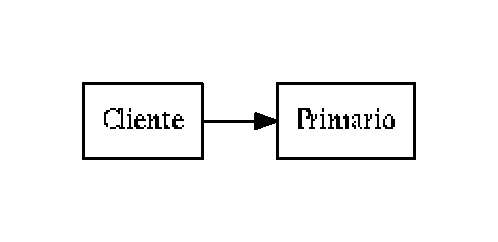
\includegraphics{graphviz-56fce8410a8ce23b6d99c6365600fd200eb47f9c.pdf}


\section{Replica Set}
\label{contents/desplieguesTipo:replica-set}\begin{itemize}
\item {} 
Máximo 1 primario

\item {} 
Máximo 11 secundarios

\item {} 
Escrituras solo en primario

\item {} 
Se pueden hacer lecturas conectándose a un secundario

\end{itemize}

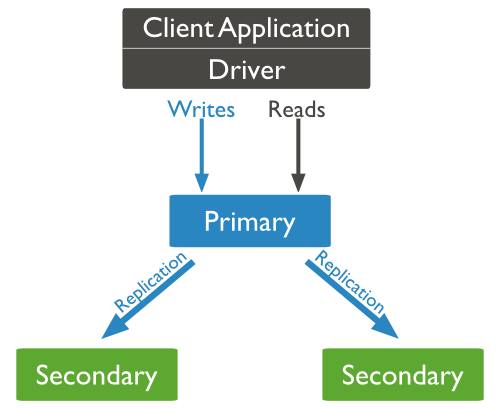
\includegraphics{replica-set-read-write-operations-primary.png}


\section{Sharded cluster}
\label{contents/desplieguesTipo:sharded-cluster}
A través del config server se sabe a que replicaSet (shard) se puede escribir/leer
Config servers posibles:
\begin{itemize}
\item {} 
1 - Usado para pruebas

\item {} 
3 - Usado para producción. Provee tolerancia a fallos

\end{itemize}

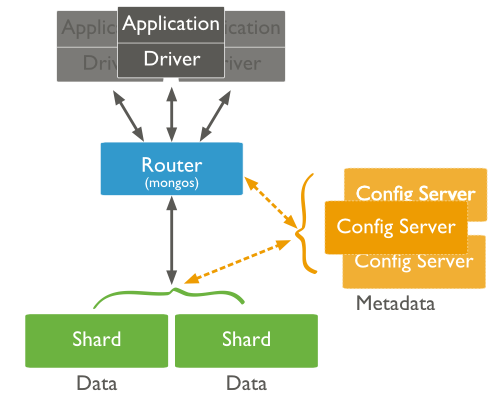
\includegraphics{sharded-cluster.png}


\chapter{Línea de comandos}
\label{contents/comandos::doc}\label{contents/comandos:linea-de-comandos}\begin{quote}\begin{description}
\item[{mongod}] \leavevmode
primary daemon process for the MongoDB system

\item[{mongos}] \leavevmode
“MongoDB Shard,” routing service for MongoDB shard configurations

\item[{mongo}] \leavevmode
interactive JavaScript shell interface to MongoDB

\item[{mongodump}] \leavevmode
utility for creating a binary export

\item[{mongorestore}] \leavevmode
writes data from a binary database dump created by mongodump to a MongoDB instance

\item[{bsondump}] \leavevmode
The bsondump converts BSON files into human-readable formats, including JSON

\item[{mongooplog}] \leavevmode
simple tool that polls operations from the replication oplog of a remote server, and applies them to the local server

\item[{mongoimport}] \leavevmode
import content from a JSON, CSV, or TSV export created by mongoexport

\item[{mongoexport}] \leavevmode
produces a JSON or CSV export of data stored in a MongoDB instance

\item[{mongostat}] \leavevmode
quick overview of the status of a currently running mongod or mongos instance

\item[{mongotop}] \leavevmode
method to track the amount of time a MongoDB instance spends reading and writing data.

\item[{mongosniff}] \leavevmode
low-level operation tracing/sniffing view into database activity in real time

\item[{mongoperf}] \leavevmode
check disk I/O performance independently of MongoDB

\item[{mongofiles}] \leavevmode
makes it possible to manipulate files stored in your MongoDB instance in GridFS objects from the command line

\end{description}\end{quote}


\section{mongod}
\label{contents/comandos:mongod}
\begin{Verbatim}[commandchars=\\\{\}]
[\PYGZhy{}\PYGZhy{}dbpath]                          default= /data/db, c:\PYGZbs{}data\PYGZbs{}db
[\PYGZhy{}\PYGZhy{}port]                            default=27017
[\PYGZhy{}\PYGZhy{}journal \textbar{} \PYGZhy{}\PYGZhy{}nojournal]           active by default on 64 bits
[\PYGZhy{}\PYGZhy{}smallfiles]
[\PYGZhy{}\PYGZhy{}nssize \PYGZlt{}MB\PYGZgt{}]                     max 2GB
[\PYGZhy{}\PYGZhy{}noprealloc]
[\PYGZhy{}\PYGZhy{}logpath]
[\PYGZhy{}\PYGZhy{}logappend]
[\PYGZhy{}\PYGZhy{}fork]                            Not supported on windows
[\PYGZhy{}\PYGZhy{}config\textbar{}\PYGZhy{}f \PYGZlt{}ASCII configFile\PYGZgt{}]
[\PYGZhy{}\PYGZhy{}replSet \PYGZlt{}rsName\PYGZgt{}]
[\PYGZhy{}\PYGZhy{}oplogSize \PYGZlt{}MG\PYGZgt{}]                  default=5\PYGZpc{} free space
[\PYGZhy{}\PYGZhy{}shardsvr]
[\PYGZhy{}\PYGZhy{}configsvr]
[\PYGZhy{}\PYGZhy{}auth]
[\PYGZhy{}\PYGZhy{}keyFile \PYGZlt{}path to file\PYGZgt{}]
[\PYGZhy{}\PYGZhy{}syncdelay 45]                    seconds between disk syncs
[\PYGZhy{}vvvvv]                            Verbose level
\end{Verbatim}

\textbf{Data File Allocation}.

Each database will have at least two data files, one ending in .ns and the rest in integers starting with 0.

The .ns file stores metadata about namespaces (collections and indexes). The number of namespaces is
proportional to the size of the .ns file. Each database can have up to 24,000 namespaces by default, although
the size of these files, and thus the number of namespaces, can be increased with the \code{-{-}nssize} option (up
to 2GB).

By default, datafiles start at 64MB and double in size with each additional datafile, up to 2GB. Additionally,
on some platforms, mongod allocates one more numbered data file than it needs, to improve throughput.
Thus, it’s possible for allocated size to be much larger than data size. If this presents a problem, you can
use some combination of server options:

\begin{Verbatim}[commandchars=\\\{\}]
\PYGZhy{}\PYGZhy{}smallfiles    // quarters the sizes of data files
\PYGZhy{}\PYGZhy{}noprealloc    // inhibits preallocation of extra files
\end{Verbatim}

\textbf{The Lock File}

\code{mongod.lock} contains PID. When the server shuts down cleanly, it truncates the lock file to length 0.

\textbf{Journal Subdirectory}

Activated by default on x86\_64 machines. Directory \code{journal}.

\begin{notice}{note}{Note:}
Todos los servidores comparten el mismo journal.
\end{notice}

\textbf{Log Files}

Default: standard output.

\code{-{-}logpath /var/mongodb/mongodb.log -{-}logappend} allows to write the log into a file.

The database includes a command to rotate log files:

\begin{Verbatim}[commandchars=\\\{\}]
\PYG{n}{db}\PYG{o}{.}\PYG{n}{adminCommand}\PYG{p}{(} \PYG{p}{\PYGZob{}} \PYG{l+s}{\PYGZdq{}}\PYG{l+s}{logRotate}\PYG{l+s}{\PYGZdq{}} \PYG{p}{:} \PYG{l+m+mi}{1} \PYG{p}{\PYGZcb{}} \PYG{p}{)} \PYG{p}{;}
\end{Verbatim}

\textbf{Config files}

All of these options can be specified in a config file. Any option that takes an argument is specified as option
= argument. Options that don’t take arguments are specified as option = true:

\begin{Verbatim}[commandchars=\\\{\}]
fork = true
\PYGZsh{} vvv = true
logpath = /var/mongodb/mongodb.log
\end{Verbatim}

Since mongodb 2.6 version, a new YALM format is introduced. Example:

\begin{Verbatim}[commandchars=\\\{\}]
\PYG{l+lScalar+lScalarPlain}{systemLog}\PYG{p+pIndicator}{:}
  \PYG{l+lScalar+lScalarPlain}{destination}\PYG{p+pIndicator}{:} \PYG{l+lScalar+lScalarPlain}{file}
  \PYG{l+lScalar+lScalarPlain}{path}\PYG{p+pIndicator}{:} \PYG{l+lScalar+lScalarPlain}{/home/vagrant/mongodata/singledb/db.log}
  \PYG{l+lScalar+lScalarPlain}{logAppend}\PYG{p+pIndicator}{:} \PYG{l+lScalar+lScalarPlain}{true}
\PYG{l+lScalar+lScalarPlain}{processManagement}\PYG{p+pIndicator}{:}
  \PYG{l+lScalar+lScalarPlain}{fork}\PYG{p+pIndicator}{:} \PYG{l+lScalar+lScalarPlain}{true}
\PYG{l+lScalar+lScalarPlain}{net}\PYG{p+pIndicator}{:}
  \PYG{l+lScalar+lScalarPlain}{port}\PYG{p+pIndicator}{:} \PYG{l+lScalar+lScalarPlain}{27017}
  \PYG{l+lScalar+lScalarPlain}{http.enabled}\PYG{p+pIndicator}{:} \PYG{l+lScalar+lScalarPlain}{true}
\PYG{l+lScalar+lScalarPlain}{storage}\PYG{p+pIndicator}{:}
  \PYG{l+lScalar+lScalarPlain}{dbPath}\PYG{p+pIndicator}{:} \PYG{l+lScalar+lScalarPlain}{/home/vagrant/mongodata/singledb/db}
  \PYG{l+lScalar+lScalarPlain}{preallocDataFiles}\PYG{p+pIndicator}{:} \PYG{l+lScalar+lScalarPlain}{false}
  \PYG{l+lScalar+lScalarPlain}{smallFiles}\PYG{p+pIndicator}{:} \PYG{l+lScalar+lScalarPlain}{true}
  \PYG{l+lScalar+lScalarPlain}{journal}\PYG{p+pIndicator}{:}
    \PYG{l+lScalar+lScalarPlain}{enabled}\PYG{p+pIndicator}{:} \PYG{l+lScalar+lScalarPlain}{true}

\PYG{c+c1}{\PYGZsh{} Otras secciones no probadas (obtenidas wiki online)}
\PYG{l+lScalar+lScalarPlain}{setParameter}\PYG{p+pIndicator}{:}
\PYG{l+lScalar+lScalarPlain}{security}\PYG{p+pIndicator}{:}
  \PYG{l+lScalar+lScalarPlain}{...}
\PYG{l+lScalar+lScalarPlain}{operationProfiling}\PYG{p+pIndicator}{:}
  \PYG{l+lScalar+lScalarPlain}{...}
\PYG{l+lScalar+lScalarPlain}{replication}\PYG{p+pIndicator}{:}
  \PYG{l+lScalar+lScalarPlain}{...}
\PYG{l+lScalar+lScalarPlain}{sharding}\PYG{p+pIndicator}{:}
  \PYG{l+lScalar+lScalarPlain}{...}
\PYG{l+lScalar+lScalarPlain}{auditLog}\PYG{p+pIndicator}{:}
  \PYG{l+lScalar+lScalarPlain}{...}
\PYG{l+lScalar+lScalarPlain}{snmp}\PYG{p+pIndicator}{:}
  \PYG{l+lScalar+lScalarPlain}{...}
\end{Verbatim}


\section{mongorestore}
\label{contents/comandos:mongorestore}
\begin{Verbatim}[commandchars=\\\{\}]
mongorestore (.exe) \PYGZhy{}d digg sampledata/dump/digg
mongorestore (.exe) \PYGZhy{}d training \PYGZhy{}c scores sampledata/dump/training/scores.bson
\end{Verbatim}


\section{mongoimport}
\label{contents/comandos:mongoimport}
\begin{Verbatim}[commandchars=\\\{\}]
mongoimport (.exe) \PYGZhy{}d twitter \PYGZhy{}c tweets sampledata/twitter.json
\end{Verbatim}


\chapter{Documentos}
\label{contents/documents::doc}\label{contents/documents:documentos}
Ejemplo documento JSON en MongoDB:

\begin{Verbatim}[commandchars=\\\{\}]
\PYGZob{}
    \PYGZdq{}\PYGZus{}id\PYGZdq{} : ObjectId(\PYGZdq{}4ba267dc238d3ba3ca000001\PYGZdq{}),
    \PYGZdq{}href\PYGZdq{} : \PYGZdq{}http://digg.com/people/Jedi\PYGZus{}apology\PYGZdq{},
    \PYGZdq{}title\PYGZdq{} : \PYGZdq{}’Jedi’ believer gets an apology!\PYGZdq{},
    \PYGZdq{}comments\PYGZdq{} : 153,
    \PYGZdq{}container\PYGZdq{} : \PYGZob{}
        \PYGZdq{}name\PYGZdq{} : \PYGZdq{}Offbeat\PYGZdq{},
        \PYGZdq{}short\PYGZus{}name\PYGZdq{} : \PYGZdq{}offbeat\PYGZdq{}
    \PYGZcb{},
    \PYGZdq{}submit\PYGZus{}date\PYGZdq{} : 1268771801,
    \PYGZdq{}topic\PYGZdq{} : \PYGZob{}
        \PYGZdq{}name\PYGZdq{} : \PYGZdq{}People\PYGZdq{},
        \PYGZdq{}short\PYGZus{}name\PYGZdq{} : \PYGZdq{}people\PYGZdq{}
    \PYGZcb{},
    \PYGZdq{}promote\PYGZus{}date\PYGZdq{} : 1268915964,
    \PYGZdq{}id\PYGZdq{} : \PYGZdq{}19970068\PYGZdq{},
    \PYGZdq{}media\PYGZdq{} : \PYGZdq{}news\PYGZdq{},
    \PYGZdq{}diggs\PYGZdq{} : 404
\PYGZcb{}
\end{Verbatim}


\chapter{CRUD - MongoDB Shell}
\label{contents/shell:crud-mongodb-shell}\label{contents/shell::doc}
Se accede con el comando \code{mongo}.

La base de datos por defecto es \code{test}.

Si se pasa la función sin paréntisis, el shell pinta la definición. Ej.: \code{db.startup\_log.findOne}

Ejemplos comandos básicos:

\begin{Verbatim}[commandchars=\\\{\}]
show dbs \textbar{} db.adminCommand(\PYGZob{}\PYGZdq{}listDatabases\PYGZdq{}: 1\PYGZcb{})
use \PYGZlt{}dbname\PYGZgt{}
show collections \textbar{} show tables \textbar{} db.getCollectionNames()
db.\PYGZlt{}col\PYGZgt{}.findOne()
db.\PYGZlt{}col\PYGZgt{}.find()
db.\PYGZlt{}col\PYGZgt{}.insert(\PYGZlt{}jsonObject\PYGZgt{})
\end{Verbatim}

\textbf{Document Data Types}

It’s sometimes useful to see the size of an object in BSON. You can do that like so

\begin{Verbatim}[commandchars=\\\{\}]
\PYG{n}{Object}\PYG{o}{.}\PYG{n}{bsonsize}\PYG{p}{(} \PYG{p}{\PYGZob{}} \PYG{l+s}{\PYGZdq{}}\PYG{l+s}{user.name}\PYG{l+s}{\PYGZdq{}} \PYG{p}{:} \PYG{l+s}{\PYGZdq{}}\PYG{l+s}{Emma Smith}\PYG{l+s}{\PYGZdq{}} \PYG{p}{\PYGZcb{}} \PYG{p}{)} \PYG{p}{;}
\PYG{n}{Object}\PYG{o}{.}\PYG{n}{bsonsize}\PYG{p}{(} \PYG{n}{db}\PYG{o}{.}\PYG{n}{tweets}\PYG{o}{.}\PYG{n}{findOne}\PYG{p}{(} \PYG{p}{\PYGZob{}} \PYG{l+s}{\PYGZdq{}}\PYG{l+s}{user.name}\PYG{l+s}{\PYGZdq{}} \PYG{p}{:} \PYG{l+s}{\PYGZdq{}}\PYG{l+s}{Emma Smith}\PYG{l+s}{\PYGZdq{}} \PYG{p}{\PYGZcb{}} \PYG{p}{)} \PYG{p}{)} \PYG{p}{;}
\end{Verbatim}

You can also query objects by BSON type. Here’s how to find all stories where href is a string.

\begin{Verbatim}[commandchars=\\\{\}]
use digg
db.stories.find( \PYGZob{} \PYGZdq{}href\PYGZdq{} : \PYGZob{} \PYGZdq{}\PYGZdl{}type\PYGZdq{} : 2 \PYGZcb{} \PYGZcb{} ) ;
\end{Verbatim}

Cargar desde un fichero:

\begin{Verbatim}[commandchars=\\\{\}]
\PYG{n}{load}\PYG{p}{(}\PYG{l+s}{\PYGZdq{}}\PYG{l+s}{testIndex.js}\PYG{l+s}{\PYGZdq{}}\PYG{p}{)}
\end{Verbatim}


\section{Inserts}
\label{contents/shell:inserts}
\begin{Verbatim}[commandchars=\\\{\}]
\PYG{n}{db}\PYG{o}{.}\PYG{n}{people}\PYG{o}{.}\PYG{n}{insert}\PYG{p}{(} \PYG{p}{\PYGZob{}} \PYG{l+s}{\PYGZdq{}}\PYG{l+s}{name}\PYG{l+s}{\PYGZdq{}} \PYG{p}{:} \PYG{l+s}{\PYGZdq{}}\PYG{l+s}{Smith}\PYG{l+s}{\PYGZdq{}}\PYG{p}{,} \PYG{l+s}{\PYGZdq{}}\PYG{l+s}{age}\PYG{l+s}{\PYGZdq{}}\PYG{p}{:} \PYG{l+m+mi}{30} \PYG{p}{\PYGZcb{}} \PYG{p}{)} \PYG{p}{;}
\end{Verbatim}


\section{Queries}
\label{contents/shell:queries}
\begin{Verbatim}[commandchars=\\\{\}]
\PYG{n}{db}\PYG{o}{.}\PYG{n}{scores}\PYG{o}{.}\PYG{n}{find}\PYG{p}{(} \PYG{p}{\PYGZob{}} \PYG{l+s}{\PYGZdq{}}\PYG{l+s}{score}\PYG{l+s}{\PYGZdq{}} \PYG{p}{:} \PYG{p}{\PYGZob{}} \PYG{l+s}{\PYGZdq{}}\PYG{l+s}{\PYGZdl{}gte}\PYG{l+s}{\PYGZdq{}} \PYG{p}{:} \PYG{l+m+mi}{70} \PYG{p}{\PYGZcb{}} \PYG{p}{\PYGZcb{}} \PYG{p}{)} \PYG{p}{;}
\end{Verbatim}

\textbf{Operators}:
\begin{itemize}
\item {} 
\$gt / \$gte / \$lt / \$lte

\item {} 
\$ne

\item {} 
\$in / \$nin. puede ser usado tanto con números, como cualquier tipo de dato (strings, ...)

\item {} 
\$mod

\item {} 
\$regex/\$options,

\item {} 
\$all

\item {} 
\$size. Consulta si el array es del tamaño que pasemos

\item {} 
\$exists. Comprueba si existe un campo

\item {} 
\$type. Comprueba si un campo es de un tipo concreto, hay que usar el número del tipo (BSON).

\item {} 
\$not

\item {} 
\$or / \$nor

\item {} 
\$elemMatch,

\item {} 
\$where (try not to use \$where !) \textbf{Full collection scan}. En breve quedará obsoleto y siempre tendrá valores javascript (aunque estemos desarrollando en otro lenguage)

\end{itemize}

In order to query into subdocuments, you must use ``Dot notation'': \code{db.collection.find( \{ "x.y" : 10 \} );}

\textbf{Queries and arrays}

Queries that examine arrays will compare each element in the array with the argument to the matching
predicate. For example, both

\begin{Verbatim}[commandchars=\\\{\}]
\PYG{n}{db}\PYG{o}{.}\PYG{n}{collection}\PYG{o}{.}\PYG{n}{find}\PYG{p}{(} \PYG{p}{\PYGZob{}} \PYG{l+s}{\PYGZdq{}}\PYG{l+s}{x}\PYG{l+s}{\PYGZdq{}} \PYG{p}{:} \PYG{l+m+mi}{2} \PYG{p}{\PYGZcb{}} \PYG{p}{)} \PYG{p}{;}
\end{Verbatim}

and

\begin{Verbatim}[commandchars=\\\{\}]
\PYG{n}{db}\PYG{o}{.}\PYG{n}{collection}\PYG{o}{.}\PYG{n}{find}\PYG{p}{(} \PYG{p}{\PYGZob{}} \PYG{l+s}{\PYGZdq{}}\PYG{l+s}{x}\PYG{l+s}{\PYGZdq{}} \PYG{p}{:} \PYG{p}{\PYGZob{}} \PYG{l+s}{\PYGZdq{}}\PYG{l+s}{\PYGZdl{}gt}\PYG{l+s}{\PYGZdq{}} \PYG{p}{:} \PYG{l+m+mi}{4} \PYG{p}{\PYGZcb{}} \PYG{p}{\PYGZcb{}} \PYG{p}{)} \PYG{p}{;}
\end{Verbatim}

will match documents where x is the array {[} 1, 2, 5 {]}. (In the first case, 2 is present in the array; in the
second case, at least one element of the array is greater than 4.)

\textbf{Subset of fields (projections)}

\begin{Verbatim}[commandchars=\\\{\}]
db.scores.find( \PYGZob{}\PYGZcb{} , \PYGZob{} \PYGZdq{}score\PYGZdq{} : 1 \PYGZcb{} ) ; // only includes score and \PYGZus{}id
db.scores.find( \PYGZob{}\PYGZcb{} , \PYGZob{} \PYGZdq{}score\PYGZdq{} : 0 \PYGZcb{}) ; // includes everything but score
\end{Verbatim}

\textbf{Cursors}

To query MongoDB is to instantiate a cursor. You can also get more control using \code{hasNext()}, \code{next()} and \code{forEach()}

\begin{Verbatim}[commandchars=\\\{\}]
var cursor = db.scores.find() ;
while ( cursor.hasNext() ) printjson( cursor.next() ) ;
db.scores.find().forEach( function(x)\PYGZob{} printjson( x ) \PYGZcb{} ) ;
db.scores.find().forEach( printjson ) ;
cursor.forEach // without () prints source
\end{Verbatim}

With \code{sort()}, \code{skip()}, and \code{limit()} you can control the results of the cursor

\begin{notice}{note}{Note:}
el cursor tiene un tiempo de vida que suelen ser unos 10 minutos.
\end{notice}


\section{Updates}
\label{contents/shell:updates}
\begin{notice}{danger}{Danger:}
Without \code{\$set} operator, full document is replaced
\begin{alltt}
db.stuff.update( \{ ``\_id'' : 123 \} , \{ ``hello'' : ``world'' \} ) ; // Replace full document
db.stuff.update( \{ ``\_id'' : 123 \} ,
        \{ \textbf{``\$set''} : \{ ``hello'' : ``world'' \} \} ) ; // Updates hello attribute
\end{alltt}
\end{notice}

\textbf{Operators}
\begin{itemize}
\item {} 
\$set

\item {} 
\$unset

\item {} 
\$inc

\item {} 
\$push

\item {} 
\$pushAll

\item {} 
\$pull

\item {} 
\$pullAll

\item {} 
\$pop

\item {} 
\$addToSet

\item {} 
\$rename

\item {} 
\$bit

\item {} 
\$ positional operator

\end{itemize}

\textbf{Upserts and multi-update}

\code{upsert}: updates or creates if not exists.

By default, only one document is updated, you must use \code{multi} in order to update several documents

\begin{Verbatim}[commandchars=\\\{\}]
\PYG{n}{db}\PYG{o}{.}\PYG{n}{people}\PYG{o}{.}\PYG{n}{update}\PYG{p}{(} \PYG{p}{\PYGZob{}} \PYG{l+s}{\PYGZdq{}}\PYG{l+s}{name}\PYG{l+s}{\PYGZdq{}} \PYG{p}{:} \PYG{l+s}{\PYGZdq{}}\PYG{l+s}{Jones}\PYG{l+s}{\PYGZdq{}} \PYG{p}{\PYGZcb{}} \PYG{p}{,} \PYG{p}{\PYGZob{}} \PYG{l+s}{\PYGZdq{}}\PYG{l+s}{\PYGZdl{}set}\PYG{l+s}{\PYGZdq{}} \PYG{p}{:} \PYG{p}{\PYGZob{}} \PYG{l+s}{\PYGZdq{}}\PYG{l+s}{age}\PYG{l+s}{\PYGZdq{}} \PYG{p}{:} \PYG{l+m+mi}{50} \PYG{p}{\PYGZcb{}} \PYG{p}{\PYGZcb{}} \PYG{p}{,} \PYG{p}{\PYGZob{}} \PYG{l+s}{\PYGZdq{}}\PYG{l+s}{upsert}\PYG{l+s}{\PYGZdq{}} \PYG{p}{:} \PYG{n}{true} \PYG{p}{\PYGZcb{}} \PYG{p}{)} \PYG{p}{;}
\PYG{n}{db}\PYG{o}{.}\PYG{n}{people}\PYG{o}{.}\PYG{n}{update}\PYG{p}{(} \PYG{p}{\PYGZob{}} \PYG{p}{\PYGZcb{}} \PYG{p}{,} \PYG{p}{\PYGZob{}} \PYG{l+s}{\PYGZdq{}}\PYG{l+s}{\PYGZdl{}set}\PYG{l+s}{\PYGZdq{}} \PYG{p}{:} \PYG{p}{\PYGZob{}} \PYG{l+s}{\PYGZdq{}}\PYG{l+s}{city}\PYG{l+s}{\PYGZdq{}} \PYG{p}{:} \PYG{l+s}{\PYGZdq{}}\PYG{l+s}{NYC}\PYG{l+s}{\PYGZdq{}} \PYG{p}{\PYGZcb{}} \PYG{p}{\PYGZcb{}} \PYG{p}{,} \PYG{p}{\PYGZob{}} \PYG{l+s}{\PYGZdq{}}\PYG{l+s}{multi}\PYG{l+s}{\PYGZdq{}} \PYG{p}{:} \PYG{n}{true} \PYG{p}{\PYGZcb{}} \PYG{p}{)} \PYG{p}{;}
\end{Verbatim}


\chapter{Replica Set}
\label{contents/replicaSet::doc}\label{contents/replicaSet:replica-set}
\textbf{Sistema de votos para la elección de primarios}:
\begin{itemize}
\item {} 
Para que un nodo pase a primario tiene que obtener la mayoría de votos (mayor que la mitad)

\item {} 
Mínimo 3 nodos para poder tener recuperación automática. Sino no se puede decidir un nuevo primario.

\item {} 
\textbf{Árbitro}: es un nodo secundario sin almacenamiento y solo usado para las votaciones.

\item {} 
Un secundario puede tener \textbf{derecho de veto}. Cuando un secundatio tiene una fecha de actualización mayor.

\item {} 
Máximo número de nodos que pueden votar: 7
\begin{itemize}
\item {} 
Un nodo que no puede votar, si puede poner 1 veto.

\end{itemize}

\item {} 
Los secundarios tienen prioridad, por defecto = 1.

\end{itemize}

\textbf{Oplog.rs}

En los nodos del replica set, existirá la colección \code{oplog.rs} dentro de la base de datos \code{local}.
Esta colección se crea con las escrituras en el primario y se envía a los secundarios.

Es una colección de tamaño máximo donde se almacenan las operaciones de una forma idempotente.

\textbf{Lecturas en secundarios}

Hacer lecturas en los secundarios puede ser una buena idea si estamos haciendo operaciones pesadas y no nos importa que los datos no sean justo los últimos.

Al conectarse a un secundario con el comando ``mongo'', no nos permite lecturas por defecto, para habilitarlas debemos ejecutar:

\begin{Verbatim}[commandchars=\\\{\}]
\PYG{n}{rs}\PYG{o}{.}\PYG{n}{slaveOk}\PYG{p}{(}\PYG{p}{)}
\end{Verbatim}

\textbf{Mantenimientos y upgrades}.

Para mantenimientos de los servidores y actualizaciones del software, primero se deberían hacer en los secundarios.


\section{Write concerns}
\label{contents/replicaSet:write-concerns}\begin{itemize}
\item {} 
\textbf{w:0}. Mando y espero solo el ack de la red

\item {} 
\textbf{w:1}. \emph{Valor por defecto} en standalone y primarios de replica set. Cuando la escritura ha sido hecha en la memoria del servidor, aunque no en disco ni replicada.

\item {} 
\textbf{w:n (siendo n\textgreater{}1)}. Cuando se ha confirmado en n nodos (primario y n-1 secundarios).

\item {} 
\textbf{w:''majority''}. Cuando se ha confirmado en la mayoría de los miembros del replica set.

\item {} 
\textbf{w:\textless{}tag set\textgreater{}}. Cuando se ha confirmado en los nodos configurados con el tag dado.

\item {} 
\textbf{j:true}. Espera a la escritura en el journal para devolver la confirmación.

\item {} 
\textbf{wtimeout:\textless{}ms\textgreater{}}. Timeout en milisegundos que se espera para confirmación de secundarios. Solo tiene sentido con w\textgreater{}1.

\end{itemize}


\section{Read Preference modes}
\label{contents/replicaSet:read-preference-modes}\begin{itemize}
\item {} 
\textbf{primary}. Valor por defecto. Siempre se lee en el primario

\item {} 
\textbf{primaryPrefered}. Siempre en el primario a no ser que no esté disponible, en este caso se permiten secundarios.

\item {} 
\textbf{secondary}. Solo se lee de secundarios.

\item {} 
\textbf{secondaryPrefered}. Se lee de secundarios a no ser que ninguno esté disponible.

\item {} 
\textbf{nearest}. Lee del mas cercano (nodo con menos latencia en la red) sea primario o secundario.

\end{itemize}


\section{Datacenters}
\label{contents/replicaSet:datacenters}
Como ya se ha dicho, para auto-recuperación de un replica set necesitamos al menos 3 nodos (si hay solo 2 y se cae el primario, el secundario no tiene votos suficientes para pasar a primario). Repartiendo los nodos en datacenters:

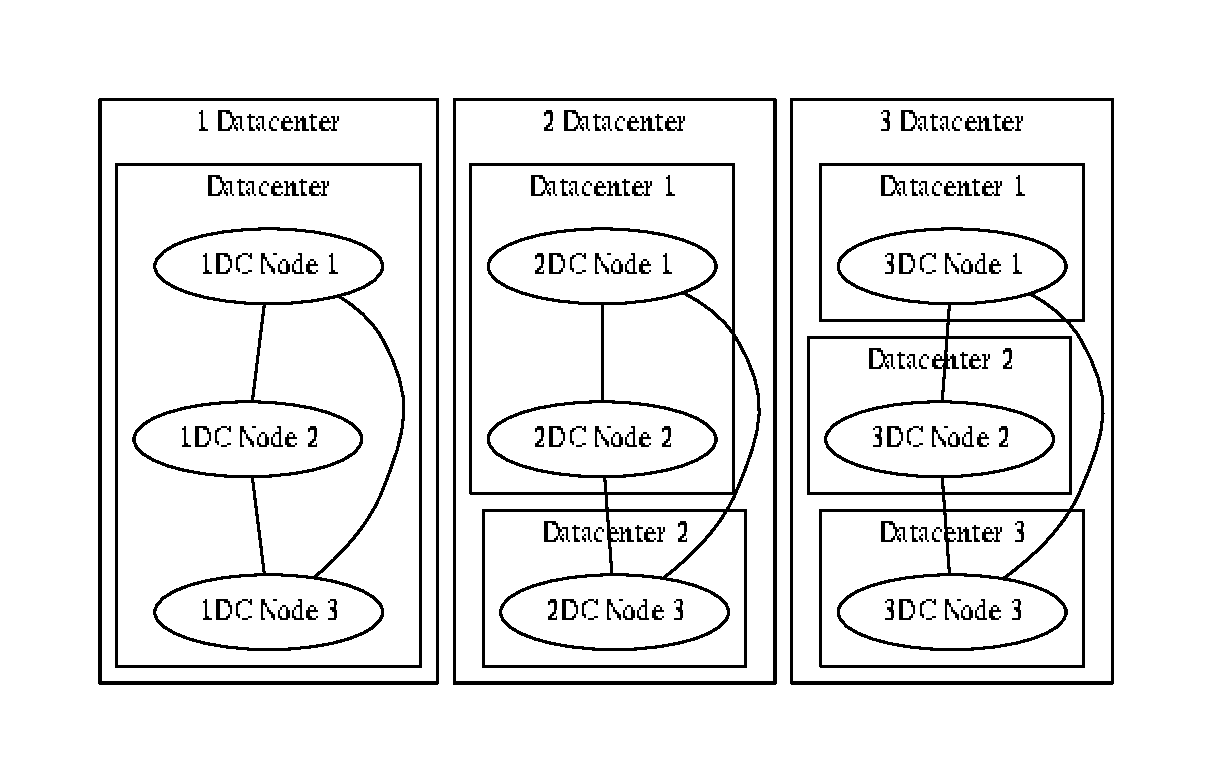
\includegraphics{graphviz-7e3673d918e91bd6856d148078d48699ab39ecdb.pdf}

Podemos ver que la única configuración para poder recuperarse automáticamente ante la caída/destrucción de un data center (DR = Disaster Recovery) es usar como mínimo 3 datacenters.

Si usamos 1 y se pierde, perdemos todo.

Si usamos 2, podríamos recuperarnos en el caso de que el datacenter que se pierda sea el que contiene 1 nodo, en otro caso, no.


\section{Configuración.}
\label{contents/replicaSet:configuracion}
\textbf{Configurando un replica set añadiendo secundarios}:
\begin{itemize}
\item {} 
Se levantan los servidores con el nombre del replica set
\begin{itemize}
\item {} 
\code{\$ mongod ... -{-}replSet set0}. Si se configura desde linea de comandos. ``set0'' es el nombre del replica set

\item {} 
\code{replSet=set0}. Si se configura en fichero de configuración con formato antiguo

\item {} 
\code{replication.replSetName: set0}. Si se configura en el fichero de configuración con formato YAML

\end{itemize}

\item {} 
Nos conectamos al nodo que será el primario
\begin{itemize}
\item {} 
Con \code{rs.status()} podemos comprobar que no está inicializado el replica set

\item {} 
Con \code{rs.conf()} también veremos datos de la configuración del replica set

\end{itemize}

\item {} 
Con \code{rs.initiate()} iniciamos el replica set que solo tendrá este nodo actualmente
y el shell nos debería cambiar a \code{set0:PRIMARY\textgreater{}}.

\item {} 
Para añadir otros nodos \code{rs.add("\textless{}hostname\textgreater{}:\textless{}port\textgreater{}")}. Ejemplo: \code{rs.add("precise32:28002")}.
\begin{itemize}
\item {} 
También es posible pasar un documento en vez de un string con la configuración del nodo.

\item {} 
Los secundarios deben ser añadidos desde el primario

\end{itemize}

\end{itemize}

\textbf{Configurando un replica set pasando la configuración de todos los nodos:}

Para ello, en vez de inicializar con una configuración vacía, pasamos al comando ``initiate'' la configuración:

\begin{Verbatim}[commandchars=\\\{\}]
\PYG{n}{config} \PYG{o}{=} \PYG{p}{\PYGZob{}} \PYG{l+s}{\PYGZdq{}}\PYG{l+s}{\PYGZus{}id}\PYG{l+s}{\PYGZdq{}}\PYG{p}{:} \PYG{l+s}{\PYGZdq{}}\PYG{l+s}{set0}\PYG{l+s}{\PYGZdq{}}\PYG{p}{,} \PYG{l+s}{\PYGZdq{}}\PYG{l+s}{members}\PYG{l+s}{\PYGZdq{}} \PYG{p}{:} \PYG{p}{[}
    \PYG{p}{\PYGZob{}}\PYG{l+s}{\PYGZdq{}}\PYG{l+s}{\PYGZus{}id}\PYG{l+s}{\PYGZdq{}} \PYG{p}{:} \PYG{l+m+mi}{0}\PYG{p}{,} \PYG{l+s}{\PYGZdq{}}\PYG{l+s}{host}\PYG{l+s}{\PYGZdq{}} \PYG{p}{:} \PYG{l+s}{\PYGZdq{}}\PYG{l+s}{localhost:27017}\PYG{l+s}{\PYGZdq{}} \PYG{p}{\PYGZcb{}}\PYG{p}{,}
    \PYG{p}{\PYGZob{}}\PYG{l+s}{\PYGZdq{}}\PYG{l+s}{\PYGZus{}id}\PYG{l+s}{\PYGZdq{}} \PYG{p}{:} \PYG{l+m+mi}{1}\PYG{p}{,} \PYG{l+s}{\PYGZdq{}}\PYG{l+s}{host}\PYG{l+s}{\PYGZdq{}} \PYG{p}{:} \PYG{l+s}{\PYGZdq{}}\PYG{l+s}{localhost:27018}\PYG{l+s}{\PYGZdq{}} \PYG{p}{\PYGZcb{}}\PYG{p}{,}
    \PYG{p}{\PYGZob{}}\PYG{l+s}{\PYGZdq{}}\PYG{l+s}{\PYGZus{}id}\PYG{l+s}{\PYGZdq{}} \PYG{p}{:} \PYG{l+m+mi}{2}\PYG{p}{,} \PYG{l+s}{\PYGZdq{}}\PYG{l+s}{host}\PYG{l+s}{\PYGZdq{}} \PYG{p}{:} \PYG{l+s}{\PYGZdq{}}\PYG{l+s}{localhost:27019}\PYG{l+s}{\PYGZdq{}} \PYG{p}{\PYGZcb{}} \PYG{p}{]}
\PYG{p}{\PYGZcb{}}

\PYG{n}{rs}\PYG{o}{.}\PYG{n}{initiate}\PYG{p}{(}\PYG{n}{config}\PYG{p}{)}
\end{Verbatim}

Valores posibles de configuración:

\begin{Verbatim}[commandchars=\\\{\}]
\PYGZob{}
  \PYGZus{}id: \PYGZlt{}string\PYGZgt{},
  version: \PYGZlt{}int\PYGZgt{},
  members: [
    \PYGZob{}
      \PYGZus{}id: \PYGZlt{}int\PYGZgt{},
      host: \PYGZlt{}string\PYGZgt{},
      arbiterOnly: \PYGZlt{}boolean\PYGZgt{},
      buildIndexes: \PYGZlt{}boolean\PYGZgt{},
      hidden: \PYGZlt{}boolean\PYGZgt{},
      priority: \PYGZlt{}number\PYGZgt{},
      tags: \PYGZlt{}document\PYGZgt{},
      slaveDelay: \PYGZlt{}int\PYGZgt{},
      votes: \PYGZlt{}number\PYGZgt{}
    \PYGZcb{},
    ...
  ],
  settings: \PYGZob{}
    getLastErrorDefaults : \PYGZlt{}document\PYGZgt{},
    chainingAllowed : \PYGZlt{}boolean\PYGZgt{},
    getLastErrorModes : \PYGZlt{}document\PYGZgt{},
    heartbeatTimeoutSecs: \PYGZlt{}int\PYGZgt{}
  \PYGZcb{}
\PYGZcb{}
\end{Verbatim}

\textbf{Reconfigurar un replica set}:

\begin{Verbatim}[commandchars=\\\{\}]
rs.reconfig(\PYGZlt{}config\PYGZgt{})
\end{Verbatim}


\section{Configuración rápida.}
\label{contents/replicaSet:configuracion-rapida}
Existe una forma de crear un replica set de forma rápida para pruebas y desarrollo, para ello necesitamos el directorio \code{/data/db}

\begin{Verbatim}[commandchars=\\\{\}]
\PYGZsh{} mkdir \PYGZhy{}p /data/db
\PYGZsh{} chown \PYGZhy{}R student:student /data
\PYGZdl{} mongo \PYGZhy{}\PYGZhy{}nodb
\PYGZgt{} var rsTest = new ReplSetTest(\PYGZob{}name: \PYGZdq{}replicaTest\PYGZdq{}, nodes: 3\PYGZcb{})
\PYGZgt{} rsTest.startSet() \PYGZam{}\PYGZam{} rsTest.initiate()
\end{Verbatim}

\begin{notice}{note}{Note:}
Una vez salgamos de la consola el réplica set se finaliza
\end{notice}

Conectarse desde consola:

\begin{Verbatim}[commandchars=\\\{\}]
\PYGZdl{} mongo \PYGZhy{}\PYGZhy{}nodb
\PYGZgt{} conn = new Mongo(\PYGZdq{}localhost:31000\PYGZdq{}) // Conectamos al primario
\PYGZgt{} db = conn.getDB(\PYGZdq{}test\PYGZdq{})
// Para conectarse al secundario
replicaTest:PRIMARY\PYGZgt{} conn = new Mongo(\PYGZdq{}localhost:31001\PYGZdq{})
replicaTest:PRIMARY\PYGZgt{} db = conn.getDB(\PYGZdq{}test\PYGZdq{})

// Volvemos al primario para insertar datos
\PYGZgt{} replicaTest:PRIMARY\PYGZgt{} use test // Esta puede no ser necesaria
\end{Verbatim}


\chapter{Sharding}
\label{contents/sharding::doc}\label{contents/sharding:sharding}
Para alto rendimiento deberíamos tener todos los índices cargados en memoria junto con el working set \footnote{
\textbf{Working set}. Datos que mas utilizamos y que nos interesa que estén en memoria directamente.
}.

La forma tradicional ante llenados de memoria es escabilidad vertical (mas memoria o disco). Mongo con los shards nos permite escalabilidad horizontal.

Funcionamiento:
\begin{itemize}
\item {} 
Para particionar una colección usamos una ``shard key''

\item {} 
Para que una colección se particione automáticamente hay que activar sharding a nivel de base de datos y a nivel de colección.

\item {} 
Las colecciones que no tengan shard se crean en el shard1 siempre (primary shard).
\begin{itemize}
\item {} 
Con \code{sh.movePrimary(...)} podemos cambiar el shard que será el primario (moverá las colecciones)

\end{itemize}

\item {} 
Según la shard key, inserta en la partición que corresponda entre ``Min value'' y ``Max value''

\item {} 
Una partición es un ``chunk'' no un ``shard''.

\item {} 
Cuando una colección es pequeña inicialmente tiene una única partición (chunk) con un tamaño máximo por defecto de 64MB. (-inf .. inf). El chunch es en base a la shard key por lo que solo existe cuando estamos en un shard y la colección está marcada para sharding.

\item {} 
Al llenarse MongoDB la divide en 2 chunks automáticamente (-inf.. 1000),{[}1000... inf) si el tamaño era de 2000 documentos todos del mismo tamaño. (realmente divide en 2 chunks de 32MB).

\item {} 
En la división de chunks se pasa uno de los nuevos chunk al otro shard (parece que no tiene por qué ser siempre, sino que es mongos quien va balanceando los chunks entre shards)

\end{itemize}


\section{shard key}
\label{contents/sharding:shard-key}\begin{itemize}
\item {} 
Una shardkey puede tener duplicados, se puede definir un nombre por ejemplo para que las escrituras vayan a varios shards
\begin{itemize}
\item {} 
Por la misma razón, el objectId no es bueno para la shardkey porque los timestamp del principio obligaría a escribir todos los últimos en el mismo shard. (incrementales y timestamps no son buena idea)

\end{itemize}

\item {} 
Una shardkey solo puede estar en un chunk, es decir, si es un valor muy usado, puede haber chunks con mas de 64MB (por ejemplo datos de los usuarios, con shardkey ``santiago'') -\textgreater{} jumbochunk.

\item {} 
Para poder crear una shard key \textbf{debe existir un índice sobre el campo o un índice compuesto que empiece por ese campo}.

\item {} 
Es inmutable

\item {} 
Los valores son inmutables

\item {} 
Limitada a 512 bytes de tamaño \emph{¿¿Comprobar??}.

\item {} 
Es usada para distribuir las queries en un shard.
\begin{itemize}
\item {} 
Por lo que se debería elegir un campo que sea usado comunmente en las queries

\end{itemize}

\item {} 
can be unique across shards (puede, que no debe) \emph{¿¿Comprobar??}.
\begin{itemize}
\item {} 
`\_id' field is only unique on individual shards

\end{itemize}

\end{itemize}

\textbf{Consideraciones sobre la shard key}. Reglas recomendadas a seguir, pero no son obligatorias ni tienen por que ser la solución óptima:
\begin{itemize}
\item {} 
Cardinality (alta cardinalidad). Veremos que nos pueden ayudar los índices compuestos.

\item {} 
Write Distributions

\item {} 
Query Isolation (que una query vaya sobre un shard siempre que sea posible)

\item {} 
Reliability

\item {} 
Index Locality

\end{itemize}

\begin{notice}{important}{Important:}
\emph{Cardinalidad y que no exista Hotspotting} (por ejemplo fecha actual, que siempre carga el mismo shard)
\end{notice}

Estrategias que se suelen usar:
\begin{itemize}
\item {} 
basado en localización (IPs pueden estar incluidas aquí)

\item {} 
incremental + (compuesto)

\item {} 
\textbf{Bucketing}. Dependiendo de lo que queramos hacer, hay que potenciar unos elementos u otros.

\item {} 
\textbf{Hash}.

\end{itemize}

Preguntas a hacer para elegir la clave:
\begin{itemize}
\item {} 
Crecimiento shard. Cómo esperamos que crecerá nuestro shard (3 nodos shard, o 100 nodos... mejor 3)

\item {} 
Latencia que sufriremos (zonas geográficas separadas)

\item {} 
CPU \& RAM (tiempo de proceso real). Cómo va a crecer el trabajo

\item {} 
Ratio de lecturas/escrituras sobre la colección

\end{itemize}


\section{mongos}
\label{contents/sharding:mongos}
Demonio intermediario al que se conecta el cliente y decide porque shard pasa la query (hace de router).

Para saber a que shard manda la query usa los \textbf{config server} (tienen información de todos los chunks y donde están esos chunk).

Sabe a donde mandar la query cuando se usa en la query la shardkey sino hay que consultarlos todos.

En la práctica, se debería poner un mongos en cada máquina cliente.


\section{config server}
\label{contents/sharding:config-server}
El config server debería ser una máquina dedicada (aunque tiene muy poca configuración). Podemos tener 1 o 3, no 2, (los 3 tienen los mismos datos), pero si se cae uno se convierten en solo lectura (de metadatos: no se puede cambiar la definición de los chunks, pero si se pueden realizar escrituras en colecciones)

Para activarlo hay que definir varios shard (puede ser un standalone o un replica set, mejor este último para tener tolerancia a fallos).

El mongos bloquea los config server durante la migración o split de chunks para que otro mongos no pueda escribir.


\section{Configuración.}
\label{contents/sharding:configuracion}
\textbf{config server}:
\begin{itemize}
\item {} 
Desde linea de comandos: \code{mongod ... -{-}configsvr}

\item {} 
Desde ficheros de configuración
\begin{itemize}
\item {} 
\code{configsvr = true} (antiguo formato)

\item {} 
\code{sharding.clusterRole: configsvr} (YAML)

\end{itemize}

\end{itemize}

El resto de las configuraciones vistas para mongod son también válidas.

\textbf{mongos}:

Desde linea de comandos: \code{mongos -{-}configdb \textless{}hostname and port of config servers\textgreater{}} (por defecto: 27017)

\begin{Verbatim}[commandchars=\\\{\}]
mongos ... \PYGZhy{}\PYGZhy{}configdb mongodbvm:28001 // configuración con 1 config server
mongos ... \PYGZhy{}\PYGZhy{}configdb mongodbvm:28001,mongodbvm:28002,mongodbvm:28003 // configuracón con 3 config servers
\end{Verbatim}

\textbf{shards}:

Cada uno de los shard estará compuesto de un servidor mongod standalone o de un replica set (mejor este caso para tolerancia a fallos)

Cada uno de los \code{mongod} deberán tener la opción \code{shardsvr} activa para indicar que forman parte de un shard cluster.
\begin{itemize}
\item {} 
Desde linea de comandos: \code{mongod ... -{-}shardsvr}

\item {} 
Desde ficheros de configuración
\begin{itemize}
\item {} 
\code{shardsvr = true} (antiguo formato)

\item {} 
\code{sharding.clusterRole: shardsvr} (YAML)

\end{itemize}

\end{itemize}

\textbf{Inicialización}:

Una vez están los demonios ejecutándose, nos conectamos con el comando \code{mongo} al demonio \code{mongos}

Una vez conectado, para añadir un shard al cluster:

\begin{Verbatim}[commandchars=\\\{\}]
sh.addShard(\PYGZdq{}localhost:27001\PYGZdq{}) // shard con un mongod standalone.
sh.addShard(\PYGZdq{}rep0/localhost:27001\PYGZdq{}) // shard con un replica set.
\end{Verbatim}

\begin{notice}{note}{Note:}
En el caso de replica sets, sólo es necesario añadir un nodo. El sistema ya obtiene toda la configuración del shard.
\end{notice}

Ahora necesitamos habilitar el sharding para la base de datos y para las colecciones que queramos:

\begin{Verbatim}[commandchars=\\\{\}]
sh.enableSharding(\PYGZdq{}dbname\PYGZdq{})
//Field es el campo que será la shard key.
sh.shardCollection(\PYGZdq{}dbname.collectionname\PYGZdq{},\PYGZob{}field:1\PYGZcb{})
\end{Verbatim}


\section{Configuración rápida.}
\label{contents/sharding:configuracion-rapida}
Al igual que los replica sets, se puede crear un shard rápido de prueba

\begin{Verbatim}[commandchars=\\\{\}]
\PYGZdl{} mongo \PYGZhy{}\PYGZhy{}nodb
\PYGZgt{} shard = new ShardingTest(\PYGZob{}name: \PYGZdq{}testShard\PYGZdq{}, shards: 3, chunksize: 26,
                rs: \PYGZob{} dbpath:\PYGZdq{}/data/shard\PYGZdq{}\PYGZcb{}\PYGZcb{})
\end{Verbatim}

Info, para mover colecciones entre tags:

\begin{Verbatim}[commandchars=\\\{\}]
mongos\PYGZgt{} db.runCommand(\PYGZob{}movePrimary: \PYGZdq{}tweets\PYGZdq{}, to: \PYGZdq{}shard0000\PYGZdq{}\PYGZcb{})

mongos\PYGZgt{} db.tweets.ensureIndex(\PYGZob{}\PYGZdq{}user.screen\PYGZus{}name\PYGZdq{}: 1\PYGZcb{})
//No lo crea automáticamente el shard key, con lo que es bueno hacerlo antes.
mongos\PYGZgt{} sh.enableSharding(\PYGZdq{}twitter\PYGZdq{})
mongos\PYGZgt{} sh.shardCollection(\PYGZdq{}twitter.tweets\PYGZdq{}, \PYGZob{}\PYGZdq{}user.screen\PYGZus{}name\PYGZdq{}:1\PYGZcb{})
\end{Verbatim}


\chapter{Backups y restauración}
\label{contents/backups::doc}\label{contents/backups:backups-y-restauracion}
DR (Disaster recovery) vs HA (High availability)

Depende de las necesidades del negocio, ¿podemos perder datos de un día? ¿cuanto tiempo podemos estar offline?...

Si perdemos un nodo, al conectar un nodo limpio se replican los datos desde el primario, pero esto significa una carga de la red al transpasar datos. Por lo que puede ser interesante cargar de un dump (o por si perdemos todo el replicaSet).


\section{Backups lógico: mongodump/mongorestore.}
\label{contents/backups:backups-logico-mongodump-mongorestore}
2 opciones:
\begin{itemize}
\item {} 
Conectándose a mongod

\item {} 
Leyendo datos del dbpath directamente

\end{itemize}

Genera para cada colección 2 ficheros:
\begin{itemize}
\item {} 
documentos en formato BSON

\item {} 
metadatos en formato JSON (estos metadatos son basicamente la definición de los índices)

\end{itemize}

Con el comando \code{bsondump} podemos ver los datos existentes en los ficheros bson.

Ejemplos:
\begin{itemize}
\item {} 
Para crear un dump completo de todas las BD del replica set (menos BD ``local'')

\begin{Verbatim}[commandchars=\\\{\}]
\PYGZdl{} mongodump \PYGZhy{}\PYGZhy{}port 27002
\end{Verbatim}

\item {} 
Dump de una sola base de datos indicando en que directorio se generará (por defecto se genera en ``dump'')

\begin{Verbatim}[commandchars=\\\{\}]
\PYGZdl{} mongodump \PYGZhy{}\PYGZhy{}port 27002 \PYGZhy{}d twitter \PYGZhy{}\PYGZhy{}out backup/misbackups/twitter
\end{Verbatim}

\end{itemize}

Para restaurar hay que conectarse al primario o sacar el secundario fuera del replicaset para cargar los datos

\begin{Verbatim}[commandchars=\\\{\}]
\PYGZdl{} mongorestore \PYGZhy{}d twitter \PYGZhy{}\PYGZhy{}port 27001 backup/misbackups/twitter/twitter
\end{Verbatim}

\begin{notice}{note}{Note:}
Si se restaura sobre una BD existente, crea los documentos nuevos si no existen (por clave primaria) o da un error (que no se muestra en consola)
\end{notice}

\textbf{Este backup puede ser inconsistente}, ya que pueden estar modificándose datos mientras se está haciendo el backup. Es decir, no bloquea la BD. Para tener un backup consistente hay 2 opciones:
\begin{itemize}
\item {} 
Bloquear: \code{db.fsyncLock()/db.fsyncUnlock()} (Esta es una buena opción para no tener que parar el servidor) o parar el servidor.

\item {} 
\code{mongodump} con \code{-{-}oplog}. Guardo las bases de datos y las operaciones ejecutadas durante el dump de la base de datos.

\end{itemize}

El fsyncLock además de bloquear hace una sincronización de memoria con disco, para que los ficheros de datos tengan los datos actualizados.

Mongodump es el mecanisco de backup mas lento. El backup físico es mas rápido, por lo que ante servidores standalone, ya que hay que bloquear para hacer backups existentes, es mejor un backup físico.

Para la opción --oplog tiene que ser un backup completo.

\begin{Verbatim}[commandchars=\\\{\}]
\PYGZdl{} mongodump \PYGZhy{}\PYGZhy{}port 27002 \PYGZhy{}\PYGZhy{}out backup/misbackups/withOpLog \PYGZhy{}\PYGZhy{}oplog
\end{Verbatim}

Esto creará además de los archivos bson y json anteriores, un nuevo fichero oplog.bson

Para restaurar un dump con oplog:

\begin{Verbatim}[commandchars=\\\{\}]
\PYGZdl{} mongorestore \PYGZhy{}\PYGZhy{}port XXX \PYGZhy{}\PYGZhy{}oplogReplay dumpFolder
\end{Verbatim}

Se podrían simular backups incrementales haciendo backups del oplog (no existe una manera nativa de backups incrementales)

\begin{Verbatim}[commandchars=\\\{\}]
\PYGZdl{} mongodump \PYGZhy{}\PYGZhy{}port 27002 \PYGZhy{}d local \PYGZhy{}c oplog.rs \PYGZhy{}\PYGZhy{}out outfolder
\PYGZdl{} mv oplog.rs.bson oplog.bson
\PYGZdl{} mongorestore \PYGZhy{}\PYGZhy{}port XXX \PYGZhy{}\PYGZhy{}oplogReplay ...
\end{Verbatim}

Para filtros selectivos en el dump tenemos ``\code{-{-}query/filter}``

Si queremos restaurar en una base de datos con distinto nombre simplemente:

\begin{Verbatim}[commandchars=\\\{\}]
\PYGZdl{} mongorestore \PYGZhy{}\PYGZhy{}port XXX \PYGZhy{}d nuevoNombre pathToDump
\end{Verbatim}


\section{Backups físicos}
\label{contents/backups:backups-fisicos}
Esta es una copia de ficheros. Y para que sean consistentes, tenemos varias opciones:
\begin{itemize}
\item {} 
shutdown / fsyncLock() ó...

\item {} 
snapshot del sistema de ficheros y luego copia de estos ficheros. Minimiza los tiempos de backup con lo que son consistentes.

\begin{notice}{important}{Important:}
Importante tener el journaling activado (para poder hacerlo sin apagar el servidor) y que el journal esté en el mismo sistema de ficheros.

Si el journal está en otro volumen, primero deberíamos hacer un bloqueo, hacer snapshots de todos los filesystems y quito el bloqueo. Luego se puede hacer la copia de ficheros a partir del snapshots.
\end{notice}

\end{itemize}

Con la copia física hay que copiar una BD completa siempre. No es posible copiar una sola colección.


\subsection{En un shard}
\label{contents/backups:en-un-shard}\begin{enumerate}
\item {} 
Hacer backup de cada uno de los replica set y de los config server.

\item {} 
Paramos balanceador

\item {} 
Paramos un config server (para que no se modifiquen los metadatos de los chunk)

\item {} 
Backup de cada shard y de un config server

\item {} 
Reiniciamos config server

\item {} 
Reiniciamos balanceador

\end{enumerate}

\emph{Info: La gente de MongoDB tiene MMS Backup. De esta forma la gente de Mongo es quien hace el backup.}


\chapter{Seguridad}
\label{contents/security::doc}\label{contents/security:seguridad}
MongoDB tiene la autenticación/autorización \textbf{desactivada por defecto}.

Esto es debido a que la primara opción de seguridad debería ser \textbf{establecer la red de cluster en una red privada protegida por cortafuegos}.


\bigskip\hrule{}\bigskip


\textbf{Cifrado}

La comunicación entre los distintos nodos y cliente no está cifrada, ni dispone de cifrado alternativo. Se podría usar aplicaciones de terceros (tunel ssh, ...). Hay que tener en cuenta que el cifrado puede penalizar el rendimiento.

Tampoco hay cifrado de datos en disco.

Lo único que hay cifrado es la contraseña de los usuarios (tanto en el servidor como en la red).


\bigskip\hrule{}\bigskip


\textbf{Autenticación:}

Tenemos 2 tipos de autenticación:

Para un \textbf{cliente}, especificando usuario y contraseña. Asociada a esta autenticación tenemos privilegios de usuarios.

Los usuarios se crean a nivel de base de datos.
\begin{itemize}
\item {} 
\code{use twitter; db.addUser("...")}. También \code{db.createUser(...)} desde la 2.6. Con este último comando podemos crear un usuario para varias BD.

\item {} 
Se guardan en la colección \code{system.users} en cada una de las BD.

\item {} 
Debemos activar la autenticación con \code{-{-}auth} en el arranque del demonio.

\item {} 
Desde localhost se permite conectar sin autenticación si no hay usuarios definidos en \code{admin.system.users}.

\end{itemize}

Para usar \textbf{autenticación con un shard o réplica set}, primero debemos generar una clave:

\begin{Verbatim}[commandchars=\\\{\}]
\PYGZdl{} openssl rand \PYGZhy{}base64 741 \PYGZgt{} mongodb\PYGZhy{}keyfile
\end{Verbatim}

Y cambiar los permisos

\begin{Verbatim}[commandchars=\\\{\}]
\PYGZdl{} chmod 600 mongodb\PYGZhy{}keyfile
\end{Verbatim}

Lo que nos queda es arrancar los replicaSet y shard con la opción \code{-{-}keyFile} (implica \code{-{-}auth})

La clave es para evitar suplantaciones de identidad de un réplica set, lo cual sería posible si se cae un elemento del réplica set y se suplanta la IP.


\bigskip\hrule{}\bigskip


\textbf{Ejemplo configuración con clave}

\begin{Verbatim}[commandchars=\\\{\}]
\PYGZsh{} Config servers
mongod \PYGZhy{}\PYGZhy{}dbpath=data/config\PYGZus{}server\PYGZus{}1 \PYGZhy{}\PYGZhy{}fork \PYGZbs{}
     \PYGZhy{}\PYGZhy{}logpath=data/config\PYGZus{}server\PYGZus{}1/mongod.log \PYGZhy{}\PYGZhy{}logappend \PYGZbs{}
     \PYGZhy{}\PYGZhy{}port 28001 \PYGZhy{}\PYGZhy{}configsvr \PYGZhy{}\PYGZhy{}keyFile data/mongodb\PYGZhy{}keyfile
mongod \PYGZhy{}\PYGZhy{}dbpath=data/config\PYGZus{}server\PYGZus{}2 \PYGZhy{}\PYGZhy{}fork \PYGZbs{}
     \PYGZhy{}\PYGZhy{}logpath=data/config\PYGZus{}server\PYGZus{}2/mongod.log \PYGZhy{}\PYGZhy{}logappend \PYGZbs{}
     \PYGZhy{}\PYGZhy{}port 28002 \PYGZhy{}\PYGZhy{}configsvr \PYGZhy{}\PYGZhy{}keyFile data/mongodb\PYGZhy{}keyfile
mongod \PYGZhy{}\PYGZhy{}dbpath=data/config\PYGZus{}server\PYGZus{}3 \PYGZhy{}\PYGZhy{}fork \PYGZbs{}
     \PYGZhy{}\PYGZhy{}logpath=data/config\PYGZus{}server\PYGZus{}3/mongod.log \PYGZhy{}\PYGZhy{}logappend \PYGZbs{}
     \PYGZhy{}\PYGZhy{}port 28003 \PYGZhy{}\PYGZhy{}configsvr \PYGZhy{}\PYGZhy{}keyFile data/mongodb\PYGZhy{}keyfile

\PYGZsh{} RS set0
mongod \PYGZhy{}\PYGZhy{}dbpath=data/rs1/db1 \PYGZhy{}\PYGZhy{}journal \PYGZhy{}\PYGZhy{}fork \PYGZbs{}
     \PYGZhy{}\PYGZhy{}logpath=data/rs1/db1/mongod.log \PYGZhy{}\PYGZhy{}logappend \PYGZhy{}\PYGZhy{}replSet set0 \PYGZhy{}\PYGZhy{}port 27001 \PYGZbs{}
     \PYGZhy{}\PYGZhy{}shardsvr \PYGZhy{}\PYGZhy{}keyFile data/mongodb\PYGZhy{}keyfile
mongod \PYGZhy{}\PYGZhy{}dbpath=data/rs1/db2 \PYGZhy{}\PYGZhy{}journal \PYGZhy{}\PYGZhy{}fork \PYGZbs{}
     \PYGZhy{}\PYGZhy{}logpath=data/rs1/db2/mongod.log \PYGZhy{}\PYGZhy{}logappend \PYGZhy{}\PYGZhy{}replSet set0 \PYGZhy{}\PYGZhy{}port 27002 \PYGZbs{}
     \PYGZhy{}\PYGZhy{}shardsvr \PYGZhy{}\PYGZhy{}keyFile data/mongodb\PYGZhy{}keyfile
mongod \PYGZhy{}\PYGZhy{}dbpath=data/rs1/db3 \PYGZhy{}\PYGZhy{}journal \PYGZhy{}\PYGZhy{}fork \PYGZbs{}
     \PYGZhy{}\PYGZhy{}logpath=data/rs1/db3/mongod.log \PYGZhy{}\PYGZhy{}logappend \PYGZhy{}\PYGZhy{}replSet set0 \PYGZhy{}\PYGZhy{}port 27003 \PYGZbs{}
     \PYGZhy{}\PYGZhy{}shardsvr \PYGZhy{}\PYGZhy{}keyFile data/mongodb\PYGZhy{}keyfile

\PYGZsh{} RS set1
mongod \PYGZhy{}\PYGZhy{}dbpath=data/rs2/db1 \PYGZhy{}\PYGZhy{}journal \PYGZhy{}\PYGZhy{}fork \PYGZbs{}
     \PYGZhy{}\PYGZhy{}logpath=data/rs2/db1/mongod.log \PYGZhy{}\PYGZhy{}logappend \PYGZhy{}\PYGZhy{}replSet set1 \PYGZhy{}\PYGZhy{}port 27101 \PYGZbs{}
     \PYGZhy{}\PYGZhy{}shardsvr \PYGZhy{}\PYGZhy{}keyFile data/mongodb\PYGZhy{}keyfile
mongod \PYGZhy{}\PYGZhy{}dbpath=data/rs2/db2 \PYGZhy{}\PYGZhy{}journal \PYGZhy{}\PYGZhy{}fork \PYGZbs{}
     \PYGZhy{}\PYGZhy{}logpath=data/rs2/db2/mongod.log \PYGZhy{}\PYGZhy{}logappend \PYGZhy{}\PYGZhy{}replSet set1 \PYGZhy{}\PYGZhy{}port 27102 \PYGZbs{}
     \PYGZhy{}\PYGZhy{}shardsvr \PYGZhy{}\PYGZhy{}keyFile data/mongodb\PYGZhy{}keyfile
mongod \PYGZhy{}\PYGZhy{}dbpath=data/rs2/db3 \PYGZhy{}\PYGZhy{}journal \PYGZhy{}\PYGZhy{}fork \PYGZbs{}
     \PYGZhy{}\PYGZhy{}logpath=data/rs2/db3/mongod.log \PYGZhy{}\PYGZhy{}logappend \PYGZhy{}\PYGZhy{}replSet set1 \PYGZhy{}\PYGZhy{}port 27103 \PYGZbs{}
     \PYGZhy{}\PYGZhy{}shardsvr \PYGZhy{}\PYGZhy{}keyFile data/mongodb\PYGZhy{}keyfile

\PYGZsh{} MongoS
mongos \PYGZhy{}\PYGZhy{}configdb mongodbvm:28001,mongodbvm:28002,mongodbvm:28003 \PYGZbs{}
     \PYGZhy{}\PYGZhy{}logpath=data/mongos1/mongos.log \PYGZhy{}\PYGZhy{}logappend \PYGZhy{}\PYGZhy{}fork \PYGZhy{}\PYGZhy{}port 28000 \PYGZbs{}
     \PYGZhy{}\PYGZhy{}keyFile data/mongodb\PYGZhy{}keyfile
\end{Verbatim}


\chapter{Monitorización y rendimiento}
\label{contents/monitor::doc}\label{contents/monitor:monitorizacion-y-rendimiento}
\textbf{mongostat}
\begin{itemize}
\item {} 
opcounters

\item {} 
resident memory size

\item {} 
page faults (cuando no lo encuentra en memoria y pasa a buscarlo a disco) Tener pocos es normal, tener muchos no es bueno, puede indicar que el working set no coje en memoria.

\item {} 
Porcentaje de bloqueos y número de operaciones esperando en colas de escritura/lectura (ar/qr)

\item {} 
(Mirar en la documentación de mongo online para ver una descripción de todos los campos)

\end{itemize}

\textbf{mongotop}

\textbf{db.currentOp(true)}. Me enseña las operaciones actuales.

\textbf{db.killOp(op\_id)}. Para matar una operación que no está bloqueando o tardando demasiado.

\textbf{db.serverStatus()}. Estado general del servidor, información del flush (veces, tiempo que tarda de media, tiempo del último), número de conexiones, información del journal

\textbf{db.stats()}

\textbf{db.\textless{}collection\textgreater{}.stats()}

\textbf{Database profiling}

\code{db.setProfilingLevel()}. Permite establecer estadísticas de las queries que está ejecutando. Por defecto tiene level 0 (no está activado). level 1 -\textgreater{} queries lentas. level 2 -\textgreater{} todas las queries

Por defecto una query se considera lenta si tarda mas de 100ms.

\code{db.setProfilingLevel(2, -1)}. Con -1 para que muestre todas las queries, 0 puede dejar queries sin mostrar por los redondeos.

Esto crea una colleción llamada \code{system.profile} en la base de datos local (no se soporta sobre un sharding)

Tendrá una sobrecarga de acceso a disco, por lo que no es normal activarlo siempre, o como mucho las queries lentas. Dejando activado todo solo en temas de log


\chapter{Optimización}
\label{contents/optimizing::doc}\label{contents/optimizing:optimizacion}\begin{itemize}
\item {} 
Se pretende optimizar las queries de lectura para alto rendimiento aunque se penalicen las escrituras.

\item {} 
MongoDB trabaja con estructuras B-Tree para los índices.

\item {} 
En la parte de sharding, no se pueden modificar los índices. \emph{Duda: ¿solo shard key o todos?}

\item {} 
Límite de índices por colección: 64

\item {} 
La ordenación en memoria sin un índice está limitada a 32MB

\item {} 
En una query solo se puede utilizar 1 índice, salvo en una query con operador \$or.
\begin{itemize}
\item {} 
En el caso del \$or se puede usar un índice por cada una de las clausulas alternativas.

\end{itemize}

\item {} 
Aunque eliminemos una colección, el índice permacene (está asociado al espacio de nombres: fichero .ns)

\end{itemize}


\section{Explain}
\label{contents/optimizing:explain}
Lo ejecutamos para la query:

\begin{Verbatim}[commandchars=\\\{\}]
\PYG{n}{db}\PYG{o}{.}\PYG{n}{users}\PYG{o}{.}\PYG{n}{find}\PYG{p}{(}\PYG{p}{)}\PYG{o}{.}\PYG{n}{explain}\PYG{p}{(}\PYG{p}{)}
\end{Verbatim}

Cuando no existe un índice nos devuelve un \code{BasicCursor}

\begin{Verbatim}[commandchars=\\\{\}]
\PYGZgt{} db.users.find(\PYGZob{}age: \PYGZob{}\PYGZdl{}gt: 80\PYGZcb{}\PYGZcb{}).explain()
\PYGZob{} \PYGZdq{}cursor\PYGZdq{} : \PYGZdq{}BasicCursor\PYGZdq{},
  \PYGZdq{}isMultiKey\PYGZdq{} : false,
  \PYGZdq{}n\PYGZdq{} : 19101,
  \PYGZdq{}nscannedObjects\PYGZdq{} : 100000,
  \PYGZdq{}nscanned\PYGZdq{} : 100000,
  \PYGZdq{}nscannedObjectsAllPlans\PYGZdq{} : 100000,
  \PYGZdq{}nscannedAllPlans\PYGZdq{} : 100000,
  \PYGZdq{}scanAndOrder\PYGZdq{} : false,
  \PYGZdq{}indexOnly\PYGZdq{} : false,
  \PYGZdq{}nYields\PYGZdq{} : 781,
  \PYGZdq{}nChunkSkips\PYGZdq{} : 0,
  \PYGZdq{}millis\PYGZdq{} : 92,
  \PYGZdq{}server\PYGZdq{} : \PYGZdq{}mongodbvm:27017\PYGZdq{},
  \PYGZdq{}filterSet\PYGZdq{} : false
\PYGZcb{}
\end{Verbatim}

\begin{notice}{tip}{Tip:}\begin{itemize}
\item {} 
\textbf{``n'' : 19101}. Número de documentos que coinciden con el criterio

\item {} 
\textbf{``nscanned'' : 100000}. Índices y/o documentos leídos

\item {} 
\textbf{``millis'' : 92}.

\item {} 
\textbf{``scanAndOrder''}. Si está a ``true'' indica que estamos utilizando un índice pero que \textbf{NO} nos sirve para ordenar.

\end{itemize}
\end{notice}


\section{Tipos de indexaciones}
\label{contents/optimizing:tipos-de-indexaciones}\begin{itemize}
\item {} 
Simple (un solo campo)

\item {} 
Compuesta (varios campos)

\item {} 
MultiKey (arrays, subdocumentos o arrays de subdocumentos)

\item {} 
TTL

\item {} 
Text

\item {} 
Geo (geoespaciales)

\item {} 
Hashed Index

\end{itemize}

Comandos:

\begin{Verbatim}[commandchars=\\\{\}]
//Crear un índice
\PYGZgt{} db.users.ensureIndex(\PYGZob{}age: 1\PYGZcb{})
//Con unicidad
\PYGZgt{} db.users.ensureIndex(\PYGZob{}name:1\PYGZcb{},\PYGZob{}unique:1\PYGZcb{})
//Elimina los duplicados si existen (dejando el primero)
\PYGZgt{} db.users.ensureIndex(\PYGZob{}name:1\PYGZcb{},\PYGZob{}unique:1, dropDups : 1\PYGZcb{})
//Índice disperso (puede o no existir el atributo)
\PYGZgt{} db.nums.ensureIndex(\PYGZob{}z:1\PYGZcb{},\PYGZob{}unique:true, sparse:true\PYGZcb{})
//Construye el índice en background
\PYGZgt{} db.nums.ensureIndex(\PYGZob{}z:1\PYGZcb{},\PYGZob{}background:true\PYGZcb{})
//Índice TTL
\PYGZgt{} db.logs.ensureIndex(\PYGZob{}creado : 1\PYGZcb{}, \PYGZob{}expireAfterSeconds: 5\PYGZcb{})
//Índice de tipo texto
\PYGZgt{} db.tweets.ensureIndex(\PYGZob{}text: \PYGZdq{}text\PYGZdq{}\PYGZcb{})
//Índice geoespacial (primera versión)
\PYGZgt{} db.tweets.ensureIndex(\PYGZob{}attrib: \PYGZdq{}2d\PYGZdq{}\PYGZcb{})
//Índice geoespacial (última versión)
\PYGZgt{} db.tweets.ensureIndex(\PYGZob{}attrib: \PYGZdq{}2dsphere\PYGZdq{}\PYGZcb{})
//Índice por hash
\PYGZgt{} db.collection.ensudeIndex( \PYGZob{}\PYGZus{}id: \PYGZdq{}hashed\PYGZdq{}\PYGZcb{})
//Para ver los índices existentes
\PYGZgt{} db.users.getIndexes()
//Para borrar un índice
\PYGZgt{} db.users.dropIndex(\PYGZdq{}city\PYGZus{}1\PYGZdq{})
//Borra todos los índices de una colección
\PYGZgt{} db.tweets.dropIndexes()
\end{Verbatim}

Cuidado con los índices dispersos y \code{\$exists}, ya que puede evitar el uso del índice u otros problemas...

Se podría insertar un z=null que sería un valor a tener en cuenta, pero no se permitiría otra tupla con z=null (por el índice único sobre z)

Durante la construcción en background podrían existir escrituras en medio, y será mas lento. A partir de la versión 2.6 se puede construir mas de un índice en background al mismo tiempo.


\section{Índice Simple.}
\label{contents/optimizing:indice-simple}\begin{itemize}
\item {} 
Indicando campo y orden

\item {} 
Se crea un índice con punteros fuertes a cada documento

\end{itemize}

\begin{Verbatim}[commandchars=\\\{\}]
\PYGZgt{} db.users.ensureIndex(\PYGZob{}age: 1\PYGZcb{})
\PYGZob{}
    \PYGZdq{}createdCollectionAutomatically\PYGZdq{} : false,
    \PYGZdq{}numIndexesBefore\PYGZdq{} : 1,
    \PYGZdq{}numIndexesAfter\PYGZdq{} : 2,
    \PYGZdq{}ok\PYGZdq{} : 1
\PYGZcb{}

\PYGZgt{} db.users.find(\PYGZob{}age: \PYGZob{}\PYGZdl{}gt: 80\PYGZcb{}\PYGZcb{}).explain()
\PYGZob{}
    \PYGZdq{}cursor\PYGZdq{} : \PYGZdq{}BtreeCursor age\PYGZus{}1\PYGZdq{},
    \PYGZdq{}isMultiKey\PYGZdq{} : false,
    \PYGZdq{}n\PYGZdq{} : 19101,
    \PYGZdq{}nscannedObjects\PYGZdq{} : 19101,
    \PYGZdq{}nscanned\PYGZdq{} : 19101,
    \PYGZdq{}nscannedObjectsAllPlans\PYGZdq{} : 19101,
    \PYGZdq{}nscannedAllPlans\PYGZdq{} : 19101,
    \PYGZdq{}scanAndOrder\PYGZdq{} : false,
    \PYGZdq{}indexOnly\PYGZdq{} : false,
    \PYGZdq{}nYields\PYGZdq{} : 149,
    \PYGZdq{}nChunkSkips\PYGZdq{} : 0,
    \PYGZdq{}millis\PYGZdq{} : 81,
    \PYGZdq{}indexBounds\PYGZdq{} : \PYGZob{}
        \PYGZdq{}age\PYGZdq{} : [
            [
                80,
                Infinity
            ]
        ]
    \PYGZcb{},
    \PYGZdq{}server\PYGZdq{} : \PYGZdq{}mongodbvm:27017\PYGZdq{},
    \PYGZdq{}filterSet\PYGZdq{} : false
\PYGZcb{}


\PYGZgt{} db.users.ensureIndex(\PYGZob{}city: 1\PYGZcb{})

\PYGZgt{} db.users.find(\PYGZob{}city: /\PYGZca{}B/i\PYGZcb{}).explain()
\PYGZob{}
    \PYGZdq{}cursor\PYGZdq{} : \PYGZdq{}BtreeCursor city\PYGZus{}1\PYGZdq{},
    \PYGZdq{}isMultiKey\PYGZdq{} : false,
    \PYGZdq{}n\PYGZdq{} : 22210,
    \PYGZdq{}nscannedObjects\PYGZdq{} : 22210,
    \PYGZdq{}nscanned\PYGZdq{} : 100000,
    \PYGZdq{}nscannedObjectsAllPlans\PYGZdq{} : 22210,
    \PYGZdq{}nscannedAllPlans\PYGZdq{} : 100000,
    \PYGZdq{}scanAndOrder\PYGZdq{} : false,
    \PYGZdq{}indexOnly\PYGZdq{} : false,
    \PYGZdq{}nYields\PYGZdq{} : 781,
    \PYGZdq{}nChunkSkips\PYGZdq{} : 0,
    \PYGZdq{}millis\PYGZdq{} : 230,
    \PYGZdq{}indexBounds\PYGZdq{} : \PYGZob{}
        \PYGZdq{}city\PYGZdq{} : [
            [
                \PYGZdq{}\PYGZdq{},
                \PYGZob{}

                \PYGZcb{}
            ],
            [
                /\PYGZca{}B/i,
                /\PYGZca{}B/i
            ]
        ]
    \PYGZcb{},
    \PYGZdq{}server\PYGZdq{} : \PYGZdq{}mongodbvm:27017\PYGZdq{},
    \PYGZdq{}filterSet\PYGZdq{} : false
\PYGZcb{}
\end{Verbatim}

\begin{notice}{tip}{Tip:}
El índice no funciona porque en este caso se está usando una expresión regular.
\end{notice}

Ante varios índices el planificador usa el índice que cree mas conveniente:

\begin{Verbatim}[commandchars=\\\{\}]
\PYGZgt{} db.users.find(\PYGZob{}city:\PYGZdq{}Barcelona\PYGZdq{},age: \PYGZob{}\PYGZdl{}gt: 80\PYGZcb{}\PYGZcb{}).explain()
\PYGZob{}
    \PYGZdq{}cursor\PYGZdq{} : \PYGZdq{}BtreeCursor city\PYGZus{}1\PYGZdq{},
    \PYGZdq{}isMultiKey\PYGZdq{} : false,
    \PYGZdq{}n\PYGZdq{} : 2137,
    \PYGZdq{}nscannedObjects\PYGZdq{} : 11192,
    \PYGZdq{}nscanned\PYGZdq{} : 11192,
    \PYGZdq{}nscannedObjectsAllPlans\PYGZdq{} : 11704,
    \PYGZdq{}nscannedAllPlans\PYGZdq{} : 12220,
    \PYGZdq{}scanAndOrder\PYGZdq{} : false,
    \PYGZdq{}indexOnly\PYGZdq{} : false,
    \PYGZdq{}nYields\PYGZdq{} : 95,
    \PYGZdq{}nChunkSkips\PYGZdq{} : 0,
    \PYGZdq{}millis\PYGZdq{} : 48,
    \PYGZdq{}indexBounds\PYGZdq{} : \PYGZob{}
        \PYGZdq{}city\PYGZdq{} : [
            [
                \PYGZdq{}Barcelona\PYGZdq{},
                \PYGZdq{}Barcelona\PYGZdq{}
            ]
        ]
    \PYGZcb{},
    \PYGZdq{}server\PYGZdq{} : \PYGZdq{}mongodbvm:27017\PYGZdq{},
    \PYGZdq{}filterSet\PYGZdq{} : false
\PYGZcb{}
\end{Verbatim}


\section{Índice Compuesto}
\label{contents/optimizing:indice-compuesto}
\begin{Verbatim}[commandchars=\\\{\}]
\PYGZgt{} db.users.ensureIndex(\PYGZob{}city: 1, age: 1\PYGZcb{})
\end{Verbatim}

Si se busca por un campo del índice se puede seguir usando un índice compuesto
siempre que este sea el primer nivel del índice (el orden importa a la hora de crear los índices compuestos).

\begin{notice}{note}{Note:}
Si se recupera solo la información que está en el índice, es una query muy rápida y se denomina \textbf{``Query Covered''}. Para esto los campos de la búsqueda y de la proyección deben estar en el índice:

\begin{Verbatim}[commandchars=\\\{\}]
\PYGZgt{} db.users.find(\PYGZob{}city:\PYGZdq{}Barcelona\PYGZdq{}\PYGZcb{}, \PYGZob{}age:1, \PYGZus{}id:0\PYGZcb{}).explain()
\end{Verbatim}
\end{notice}

Podemos añadir mas niveles al índice

\begin{Verbatim}[commandchars=\\\{\}]
\PYGZgt{} db.users.ensureIndex(\PYGZob{}city: 1, age: 1, name:1\PYGZcb{}, \PYGZob{}name:\PYGZdq{}byCityAgeAndName\PYGZdq{}\PYGZcb{}) //Con nombre

\PYGZgt{} db.users.find(\PYGZob{}city: \PYGZdq{}Barcelona\PYGZdq{}, name : /9\PYGZdl{}/\PYGZcb{}).explain()
\PYGZob{}
    \PYGZdq{}cursor\PYGZdq{} : \PYGZdq{}BtreeCursor city\PYGZus{}1\PYGZus{}age\PYGZus{}1\PYGZus{}name\PYGZus{}1\PYGZdq{},
    \PYGZdq{}isMultiKey\PYGZdq{} : false,
    \PYGZdq{}n\PYGZdq{} : 1098,
    \PYGZdq{}nscannedObjects\PYGZdq{} : 1098,
    \PYGZdq{}nscanned\PYGZdq{} : 11192,
    \PYGZdq{}nscannedObjectsAllPlans\PYGZdq{} : 3150,
    \PYGZdq{}nscannedAllPlans\PYGZdq{} : 13246,
    \PYGZdq{}scanAndOrder\PYGZdq{} : false,
    \PYGZdq{}indexOnly\PYGZdq{} : false,
    \PYGZdq{}nYields\PYGZdq{} : 103,
    \PYGZdq{}nChunkSkips\PYGZdq{} : 0,
    \PYGZdq{}millis\PYGZdq{} : 77,
    \PYGZdq{}indexBounds\PYGZdq{} : \PYGZob{}
        \PYGZdq{}city\PYGZdq{} : [
            [
                \PYGZdq{}Barcelona\PYGZdq{},
                \PYGZdq{}Barcelona\PYGZdq{}
            ]
        ],
        \PYGZdq{}age\PYGZdq{} : [
            [
                \PYGZob{}
                    \PYGZdq{}\PYGZdl{}minElement\PYGZdq{} : 1
                \PYGZcb{},
                \PYGZob{}
                    \PYGZdq{}\PYGZdl{}maxElement\PYGZdq{} : 1
                \PYGZcb{}
            ]
        ],
        \PYGZdq{}name\PYGZdq{} : [
            [
                \PYGZdq{}\PYGZdq{},
                \PYGZob{}

                \PYGZcb{}
            ],
            [
                /9\PYGZdl{}/,
                /9\PYGZdl{}/
            ]
        ]
    \PYGZcb{},
    \PYGZdq{}server\PYGZdq{} : \PYGZdq{}mongodbvm:27017\PYGZdq{},
    \PYGZdq{}filterSet\PYGZdq{} : false
\PYGZcb{}
\end{Verbatim}


\section{Índice Multikey}
\label{contents/optimizing:indice-multikey}
Cuando se hace sobre un atributo que es un array, un subdocumento o arrays de subdocumentos.

Se pueden hacer índices multikey combinandolas con ``simple'', pero es mejor que el primer nivel sea el simple

Sobre atributos de un subdocumento (no lo toma como un multiKey, pero se categoriza aquí):

\begin{Verbatim}[commandchars=\\\{\}]
\PYGZgt{} db.tweets.ensureIndex(\PYGZob{}\PYGZdq{}user.followers\PYGZus{}count\PYGZdq{} : 1, \PYGZdq{}user.friends\PYGZus{}count\PYGZdq{} : 1\PYGZcb{})

\PYGZgt{} db.tweets.find(\PYGZob{}\PYGZdq{}user.followers\PYGZus{}count\PYGZdq{} : \PYGZob{}\PYGZdl{}gt : 1000\PYGZcb{}\PYGZcb{}).explain()
\PYGZob{}
    \PYGZdq{}cursor\PYGZdq{} : \PYGZdq{}BtreeCursor user.followers\PYGZus{}count\PYGZus{}1\PYGZus{}user.frinds\PYGZus{}count\PYGZus{}1\PYGZdq{},
    \PYGZdq{}isMultiKey\PYGZdq{} : false,  \PYGZlt{}\PYGZhy{}\PYGZhy{}\PYGZhy{}\PYGZhy{}\PYGZhy{} multikey
    \PYGZdq{}n\PYGZdq{} : 5862,
    ...
\end{Verbatim}


\section{Índices TTL}
\label{contents/optimizing:indices-ttl}
Estos son los índices con tiempo de vida, como por ejemplo logs rotativos, o almacenamiento de sesiones

Existen 3 restricciones para este tipo de índices:
\begin{itemize}
\item {} 
El campo a indexar tiene que ser un ISODate (obligatorio).

\item {} 
Tiene que estar en un campo limpio, sin que esté usado en un prefijo de un índice (sin que se use en otro índice).

\item {} 
No puede ser una clave compuesta.

\end{itemize}

Ej.:

\begin{Verbatim}[commandchars=\\\{\}]
\PYGZgt{} use logger
//No se puede garantizar que sea justo a los 5s
\PYGZgt{} db.logs.ensureIndex(\PYGZob{}creado : 1\PYGZcb{}, \PYGZob{}expireAfterSeconds: 5\PYGZcb{})
\PYGZgt{} db.logs.insert(\PYGZob{}creado: new Date(),
        msg: \PYGZdq{}Prueba 001\PYGZdq{}, detalles: \PYGZdq{}Prueba 001\PYGZdq{}, nivel\PYGZus{}log: \PYGZdq{}FINE\PYGZdq{}\PYGZcb{})
\PYGZgt{} db.logs.find() // después de 5s desaparece el documento
\end{Verbatim}

Otra alternativa, expire en 0 y añadiendo la fecha de expiración en el insert:

\begin{Verbatim}[commandchars=\\\{\}]
\PYGZgt{} db.subastas.ensureIndex(\PYGZob{}fecha\PYGZus{}final:1\PYGZcb{},\PYGZob{}expireAfterSeconds: 0\PYGZcb{})
\PYGZgt{} db.subastas.insert(\PYGZob{}id:90, product: \PYGZob{}id: 4, precio: 56.8\PYGZcb{}, pujas:[],
        fecha\PYGZus{}final: new Date(\PYGZdq{}20:15:00\PYGZdq{})\PYGZcb{})
\end{Verbatim}


\section{Índices TEXT}
\label{contents/optimizing:indices-text}
Indice sobre textos complejos.

Como son lentos, es normal montarlos en background. Cuando trabajemos sobre índices TEXT siempre trabajaremos con accesos a disco.

A la hora de definir un índice, en vez de un ``1'', estableceremos un ``text''.

\begin{Verbatim}[commandchars=\\\{\}]
\PYGZgt{} db.tweets.ensureIndex(\PYGZob{}text: \PYGZdq{}text\PYGZdq{}\PYGZcb{})
\end{Verbatim}

Para hacer búsquedas sobre texto será el operador \$text (tanto en CRUD como en el framework de agregación).

\begin{Verbatim}[commandchars=\\\{\}]
\PYGZgt{} db.tweets.find(\PYGZob{}\PYGZdl{}text: \PYGZob{}\PYGZdl{}search: \PYGZdq{}preciso\PYGZdq{}\PYGZcb{}\PYGZcb{}).explain()
\end{Verbatim}

\begin{notice}{note}{Note:}
Siempre es un OR, no existe un Y.
\end{notice}

\textbf{Restricción}: Solo puede existir un único índice de tipo ``texto''.

Se puede escoger un idioma o ``none'' (por defecto es el del sistema):

\begin{Verbatim}[commandchars=\\\{\}]
\PYGZgt{} db.tweets.ensureIndex(\PYGZob{}text: \PYGZdq{}text\PYGZdq{}\PYGZcb{},\PYGZob{}default\PYGZus{}language: \PYGZdq{}fr\PYGZdq{}\PYGZcb{})
\PYGZgt{} db.tweets.ensureIndex(\PYGZob{}text: \PYGZdq{}text\PYGZdq{}\PYGZcb{},\PYGZob{}default\PYGZus{}language: \PYGZdq{}none\PYGZdq{}\PYGZcb{})

// Busca con OR
\PYGZgt{} db.tweets.find(\PYGZob{}\PYGZdl{}text: \PYGZob{}\PYGZdl{}search: \PYGZdq{}depende de la velocidad\PYGZdq{}\PYGZcb{}\PYGZcb{})

// Busqueda por frase
\PYGZgt{} db.tweets.find(\PYGZob{}\PYGZdl{}text: \PYGZob{}\PYGZdl{}search: \PYGZdq{}\PYGZbs{}\PYGZdq{}depende de la velocidad\PYGZbs{}\PYGZdq{}\PYGZdq{}\PYGZcb{}\PYGZcb{})

// Busqueda por frase AND otro término (Entre frases y palabras AND, entre palabras OR)
\PYGZgt{} db.tweets.find(\PYGZob{}\PYGZdl{}text: \PYGZob{}\PYGZdl{}search: \PYGZdq{}\PYGZbs{}\PYGZdq{}depende de la velocidad\PYGZbs{}\PYGZdq{} cosaDistinta\PYGZdq{}\PYGZcb{}\PYGZcb{})

//Especificando idioma
\PYGZgt{} db.tweets.find(\PYGZob{}\PYGZdl{}text: \PYGZob{}\PYGZdl{}search: \PYGZdq{}\PYGZbs{}\PYGZdq{}depende de la velocidad\PYGZbs{}\PYGZdq{} cosa distinta\PYGZdq{},
        \PYGZdl{}language: \PYGZdq{}es\PYGZdq{}\PYGZcb{}\PYGZcb{})
\end{Verbatim}


\section{Índices geoespaciales}
\label{contents/optimizing:indices-geoespaciales}
\textbf{Tipo ``2d''}.
\begin{itemize}
\item {} 
Plano

\item {} 
Los primeros en aparecer en Mongo.

\item {} 
Las coordenadas son sobre 100,100 (si queremos mas valores hay que especificar una opción)

\item {} 
La estructura a mantener es un array simple donde añadiremos la longitud y la latitudes ({[}long, latitud{]})

\item {} 
Se utiliza como entorno legacy

\end{itemize}

\textbf{Tipo ``2dsphere''}.
\begin{itemize}
\item {} 
El segundo que se añadió y el que se debería utilizar en la mayoría de los casos

\item {} 
Sigue la especificación de GeoJSON

\item {} 
\href{http://docs.mongodb.org/manual/tutorial/build-a-2dsphere-index/}{http://docs.mongodb.org/manual/tutorial/build-a-2dsphere-index/}

\item {} 
La localización es un subdocumento donde se define el tipo geométrico que vamos a tener (``Point'', ``Line'', ``Point{[}{]}'', ``Polygon'', *  ``Circle'')
\begin{itemize}
\item {} 
\code{\{loc: \{type : "Point", coordinates: {[}long, lat{]}\}\}}

\end{itemize}

\end{itemize}

\begin{notice}{important}{Important:}
Con ``2dsphere'' las unidades son en metros, mientras que con ``2d'' son en radianes.
\end{notice}

\begin{Verbatim}[commandchars=\\\{\}]
\PYGZgt{} db.\PYGZlt{}collection\PYGZgt{}.ensureIndex(\PYGZob{}\PYGZlt{}location field\PYGZgt{}:\PYGZdq{}2d\PYGZdq{}, \PYGZlt{}additional field\PYGZgt{}: \PYGZlt{}value\PYGZgt{}\PYGZcb{}, ...)

\PYGZgt{} db.\PYGZlt{}collection\PYGZgt{}.find( \PYGZob{} \PYGZlt{}location field\PYGZgt{} :
        \PYGZob{} \PYGZdl{}geoWithin: \PYGZob{}\PYGZdl{}box\textbar{}\PYGZdl{}polygon\textbar{}\PYGZdl{}center : \PYGZlt{}coordinates\PYGZgt{}\PYGZcb{}\PYGZcb{}\PYGZcb{})
\end{Verbatim}

Se puede usar \$near (en los 2dsphere solo??) como alternativa a \$geoWithin (cerca vs dentro de una figura)

Con \$near sale un listado de documentos ordenados por cercanía

\begin{Verbatim}[commandchars=\\\{\}]
\PYGZob{}
  \PYGZdl{}near: \PYGZob{}
     \PYGZdl{}geometry: \PYGZob{}
        type: \PYGZdq{}Point\PYGZdq{} ,
        coordinates: [ \PYGZlt{}longitude\PYGZgt{} , \PYGZlt{}latitude\PYGZgt{} ]
     \PYGZcb{},
     \PYGZdl{}maxDistance: \PYGZlt{}distance in meters\PYGZgt{},
     \PYGZdl{}minDistance: \PYGZlt{}distance in meters\PYGZgt{}
  \PYGZcb{}
\PYGZcb{}

\PYGZgt{} db.tweets.find(\PYGZob{}coordinates : \PYGZob{}\PYGZdl{}near: \PYGZob{}\PYGZdl{}geometry :
        \PYGZob{}type : \PYGZdq{}Point\PYGZdq{}, coordinates : [107.119031, \PYGZhy{}6.301964] \PYGZcb{}\PYGZcb{}\PYGZcb{}\PYGZcb{}).count()
\PYGZgt{} db.tweets.find(\PYGZob{}coordinates : \PYGZob{}\PYGZdl{}near: \PYGZob{}\PYGZdl{}geometry :
        \PYGZob{}type : \PYGZdq{}Point\PYGZdq{}, coordinates : [107.119031, \PYGZhy{}6.301964] \PYGZcb{},
        \PYGZdl{}maxDistance : 20000\PYGZcb{}\PYGZcb{}\PYGZcb{}).count() //20km de distincia máxima
\end{Verbatim}


\section{Índices Hash}
\label{contents/optimizing:indices-hash}
Desde la versión 2.4 de MongoDB

Podemos utilizar el campo que queramos y marcarlo dentro del index como ``hashed''.

En vez de trabajar con un documento de texto grande, se trabajaría con un hash para realizar la indexación. Es una buena opción para elegir como clave de shard key en determinadas colecciones.

\begin{Verbatim}[commandchars=\\\{\}]
\PYGZgt{} db.collection.ensudeIndex( \PYGZob{}\PYGZus{}id: \PYGZdq{}hashed\PYGZdq{}\PYGZcb{})
\end{Verbatim}


\chapter{Desarrollo. Introducción.}
\label{contents/developmentIntro::doc}\label{contents/developmentIntro:desarrollo-introduccion}
Tanto el diseño como a la hora de trabajar, mongodb es muy dependiente de la aplicación.

Si no se pone ``\_id'' en el insert se genera ObjectId que está compuesto de: timestamp+idMachine+pid+sequencia =\textgreater{} byte

JSON admite de tipos de datos:
\begin{itemize}
\item {} 
double

\item {} 
string

\item {} 
array

\item {} 
sub-docs

\item {} 
boolean

\item {} 
null

\end{itemize}

Para tener otros tipos de datos usamos BSON, que es mucho mas rico.

Todo lo que hagamos desde la consola, aunque sea JSON se serealiza en BSON (\href{http://bsonspec.org}{http://bsonspec.org})

Como ``\_id'' también se puede usar un documento:

\begin{Verbatim}[commandchars=\\\{\}]
\PYG{p}{\PYGZob{}}\PYG{n}{\PYGZus{}id}\PYG{p}{:} \PYG{p}{\PYGZob{}}\PYG{n}{state}\PYG{p}{:} \PYG{l+s}{\PYGZdq{}}\PYG{l+s}{ }\PYG{l+s}{\PYGZdq{}}\PYG{p}{,} \PYG{n}{city}\PYG{p}{:} \PYG{l+s}{\PYGZdq{}}\PYG{l+s}{ }\PYG{l+s}{\PYGZdq{}}\PYG{p}{\PYGZcb{}}\PYG{p}{\PYGZcb{}}
\end{Verbatim}

Hay que tener en cuenta que en estos casos influyen campos, orden y valor como clave primaria ya que lo que se tienen en cuenta como unicidad es el hash.

Esto está permitido, siendo 2 documentos distintos:

\begin{Verbatim}[commandchars=\\\{\}]
\PYGZgt{} db.lines.insert(\PYGZob{}\PYGZus{}id: \PYGZob{}number: 01, label:\PYGZdq{}002\PYGZdq{}\PYGZcb{} , origen:\PYGZdq{}or2\PYGZdq{}, destino:\PYGZdq{}destino2\PYGZdq{}\PYGZcb{})
\PYGZgt{} db.lines.insert(\PYGZob{}\PYGZus{}id: \PYGZob{}label:\PYGZdq{}002\PYGZdq{}, number:01\PYGZcb{} , origen:\PYGZdq{}or2\PYGZdq{}, destino:\PYGZdq{}destino2\PYGZdq{}\PYGZcb{})
\end{Verbatim}

Se pueden insertar arrays directamente que es mas eficiente que insertar uno por uno

\begin{Verbatim}[commandchars=\\\{\}]
\PYGZgt{} var array = [
... \PYGZob{}number:1, label:\PYGZdq{}001\PYGZdq{}\PYGZcb{},
... \PYGZob{}number:2, label:\PYGZdq{}002\PYGZdq{}\PYGZcb{}
... ]
\PYGZgt{} db.lines.insert(array)
BulkWriteResult(\PYGZob{}
\PYGZdq{}writeErrors\PYGZdq{} : [ ],
\PYGZdq{}writeConcernErrors\PYGZdq{} : [ ],
\PYGZdq{}nInserted\PYGZdq{} : 2,
\PYGZdq{}nUpserted\PYGZdq{} : 0,
\PYGZdq{}nMatched\PYGZdq{} : 0,
\PYGZdq{}nModified\PYGZdq{} : 0,
\PYGZdq{}nRemoved\PYGZdq{} : 0,
\PYGZdq{}upserted\PYGZdq{} : [ ]
\PYGZcb{})
\end{Verbatim}

En una lista, si hay un error en las operaciones, como la transaccionalidad es a nivel de documento, pueden quedar una parte de ellos insertada y la otra no.


\chapter{Desarrollo. Driver}
\label{contents/driver::doc}\label{contents/driver:desarrollo-driver}
Podemos descarganos el driver según el lenguage necesario en: \href{http://docs.mongodb.org/ecosystem/contents}{http://docs.mongodb.org/ecosystem/contents}

MongoClient -\textgreater{} Mongo (driver)

La app se comunicará con ayuda del driver al mongod (primario o secundario) o al mongoS.

MongoClient nos ayuda ya con problemas de conexion (pool) o concurrencia. Nos abre un pool de conexiones.

El objeto \code{DBObject} es usado para manejar JSON, pero es abstracto. \code{BasicDBObject} será la instancia normal a usar.

\textbf{Ejemplos trabajando con groovy}

\begin{Verbatim}[commandchars=\\\{\}]
\PYG{k+kn}{import} \PYG{n+nn}{com.mongodb.*}\PYG{o}{;}
\PYG{k+kn}{import} \PYG{n+nn}{com.mongodb.util.*}\PYG{o}{;}

\PYG{k+kd}{class} \PYG{n+nc}{TestMongoGroovyClient} \PYG{o}{\PYGZob{}}

    \PYG{k+kd}{static} \PYG{k+kt}{void} \PYG{n+nf}{main}\PYG{o}{(}\PYG{k+kt}{def} \PYG{n}{args}\PYG{o}{)} \PYG{o}{\PYGZob{}}
        \PYG{n}{MongoClient} \PYG{n}{client} \PYG{o}{=} \PYG{k}{new} \PYG{n}{MongoClient}\PYG{o}{(}\PYG{l+s+s2}{\PYGZdq{}localhost\PYGZdq{}}\PYG{o}{,} \PYG{l+m+mi}{27017}\PYG{o}{)}

        \PYG{n}{println} \PYG{n}{client}\PYG{o}{.}\PYG{n+na}{getDatabaseNames}\PYG{o}{(}\PYG{o}{)} \PYG{c+c1}{//show dbs}

        \PYG{n}{DB} \PYG{n}{twitterDB} \PYG{o}{=} \PYG{n}{client}\PYG{o}{.}\PYG{n+na}{getDB}\PYG{o}{(}\PYG{l+s+s2}{\PYGZdq{}tweeter\PYGZdq{}}\PYG{o}{)}

        \PYG{n}{println} \PYG{n}{twitterDB}\PYG{o}{.}\PYG{n+na}{getCollectionNames}\PYG{o}{(}\PYG{o}{)} \PYG{c+c1}{// show collections}

        \PYG{n}{DBCollection} \PYG{n}{tweets} \PYG{o}{=} \PYG{n}{twitterDB}\PYG{o}{.}\PYG{n+na}{getCollection}\PYG{o}{(}\PYG{l+s+s2}{\PYGZdq{}tweets\PYGZdq{}}\PYG{o}{)}

        \PYG{n}{BasicDBObject} \PYG{n}{firstTweet} \PYG{o}{=} \PYG{n}{tweets}\PYG{o}{.}\PYG{n+na}{findOne}\PYG{o}{(}\PYG{o}{)}

        \PYG{c+c1}{// Buscar los usuarios que son de Santiago de compostela}
        \PYG{n}{DBObject} \PYG{n}{query} \PYG{o}{=} \PYG{k}{new} \PYG{n}{BasicDBObject}\PYG{o}{(}
                \PYG{l+s+s2}{\PYGZdq{}user.location\PYGZdq{}}\PYG{o}{,} \PYG{l+s+s2}{\PYGZdq{}Santiago de Compostela\PYGZdq{}}\PYG{o}{)}

        \PYG{n}{tweets}\PYG{o}{.}\PYG{n+na}{find}\PYG{o}{(}\PYG{n}{query}\PYG{o}{)}\PYG{o}{.}\PYG{n+na}{each} \PYG{o}{\PYGZob{}} \PYG{n}{println} \PYG{n}{it}\PYG{o}{.}\PYG{n+na}{text} \PYG{o}{\PYGZcb{}}

        \PYG{c+c1}{// Todos aquellos usuarios que tienen mas de 100 followers}
        \PYG{k+kt}{def} \PYG{n}{query2} \PYG{o}{=} \PYG{k}{new} \PYG{n}{BasicDBObject}\PYG{o}{(}\PYG{l+s+s2}{\PYGZdq{}user.followers\PYGZus{}count\PYGZdq{}}\PYG{o}{,}
                \PYG{k}{new} \PYG{n+nf}{BasicDBObject}\PYG{o}{(}\PYG{l+s+s1}{\PYGZsq{}\PYGZdl{}gt\PYGZsq{}}\PYG{o}{,} \PYG{l+m+mi}{100}\PYG{o}{)}\PYG{o}{)}
        \PYG{n}{println} \PYG{n}{tweets}\PYG{o}{.}\PYG{n+na}{count}\PYG{o}{(}\PYG{n}{query2}\PYG{o}{)}

        \PYG{k+kt}{def} \PYG{n}{query3} \PYG{o}{=} \PYG{n}{query2}\PYG{o}{.}\PYG{n+na}{append}\PYG{o}{(}\PYG{l+s+s2}{\PYGZdq{}user.location\PYGZdq{}}\PYG{o}{,} \PYG{l+s+s2}{\PYGZdq{}London\PYGZdq{}}\PYG{o}{)}
        \PYG{n}{println} \PYG{n}{tweets}\PYG{o}{.}\PYG{n+na}{count}\PYG{o}{(}\PYG{n}{query3}\PYG{o}{)}

        \PYG{n}{String} \PYG{n}{queryStr} \PYG{o}{=} \PYG{l+s+s2}{\PYGZdq{}\PYGZob{}\PYGZsq{}user.location\PYGZsq{}: \PYGZsq{}London\PYGZsq{},}
\PYG{l+s+s2}{                \PYGZsq{}user.followers\PYGZus{}count\PYGZsq{}: \PYGZob{}\PYGZbs{}\PYGZdl{}gt: 100\PYGZcb{}\PYGZcb{}\PYGZdq{}}
        \PYG{n}{BasicDBObject} \PYG{n}{json} \PYG{o}{=} \PYG{o}{(}\PYG{n}{BasicDBObject}\PYG{o}{)} \PYG{n}{JSON}\PYG{o}{.}\PYG{n+na}{parse}\PYG{o}{(}\PYG{n}{queryStr}\PYG{o}{)}
        \PYG{n}{println} \PYG{n}{tweets}\PYG{o}{.}\PYG{n+na}{count}\PYG{o}{(}\PYG{n}{json}\PYG{o}{)}

        \PYG{n}{QueryBuilder} \PYG{n}{query4} \PYG{o}{=} \PYG{n}{QueryBuilder}\PYG{o}{.}\PYG{n+na}{start}\PYG{o}{(}
                \PYG{l+s+s2}{\PYGZdq{}user.followers\PYGZus{}count\PYGZdq{}}\PYG{o}{)}\PYG{o}{.}\PYG{n+na}{greaterThan}\PYG{o}{(}\PYG{l+m+mi}{100}\PYG{o}{)}
        \PYG{n}{println} \PYG{n}{tweets}\PYG{o}{.}\PYG{n+na}{count}\PYG{o}{(}\PYG{n}{query4}\PYG{o}{.}\PYG{n+na}{get}\PYG{o}{(}\PYG{o}{)}\PYG{o}{)}

        \PYG{c+c1}{//proyecciones}
        \PYG{n}{tweets}\PYG{o}{.}\PYG{n+na}{find}\PYG{o}{(}\PYG{n}{query4}\PYG{o}{.}\PYG{n+na}{get}\PYG{o}{(}\PYG{o}{)}\PYG{o}{,} \PYG{k}{new} \PYG{n}{BasicDBObject}\PYG{o}{(}\PYG{l+s+s2}{\PYGZdq{}text\PYGZdq{}}\PYG{o}{,} \PYG{l+m+mi}{1}\PYG{o}{)}\PYG{o}{)}\PYG{o}{.}\PYG{n+na}{limit}\PYG{o}{(}\PYG{l+m+mi}{10}\PYG{o}{)}\PYG{o}{.}\PYG{n+na}{each} \PYG{o}{\PYGZob{}}
            \PYG{n}{println} \PYG{n}{it}
        \PYG{o}{\PYGZcb{}}

        \PYG{c+c1}{// BasicDBList para manejar arrays}

    \PYG{o}{\PYGZcb{}}
\PYG{o}{\PYGZcb{}}
\end{Verbatim}

\begin{Verbatim}[commandchars=\\\{\}]
\PYG{k+kn}{import} \PYG{n+nn}{java.nio.channels.ReadPendingException}\PYG{o}{;}

\PYG{k+kn}{import} \PYG{n+nn}{com.mongodb.*}\PYG{o}{;}
\PYG{k+kn}{import} \PYG{n+nn}{com.mongodb.util.*}\PYG{o}{;}

\PYG{k+kd}{class} \PYG{n+nc}{TestWithReplicaSet} \PYG{o}{\PYGZob{}}

    \PYG{k+kd}{static} \PYG{k+kt}{void} \PYG{n+nf}{main}\PYG{o}{(}\PYG{k+kt}{def} \PYG{n}{args}\PYG{o}{)} \PYG{o}{\PYGZob{}}
        \PYG{c+c1}{// No hay que indicar cual es el primario ni nada}
        \PYG{n}{MongoClient} \PYG{n}{client} \PYG{o}{=} \PYG{k}{new} \PYG{n}{MongoClient}\PYG{o}{(}\PYG{o}{[}
            \PYG{k}{new} \PYG{n+nf}{ServerAddress}\PYG{o}{(}\PYG{l+s+s2}{\PYGZdq{}localhost\PYGZdq{}}\PYG{o}{,} \PYG{l+m+mi}{31000}\PYG{o}{)}\PYG{o}{,}
            \PYG{k}{new} \PYG{n+nf}{ServerAddress}\PYG{o}{(}\PYG{l+s+s2}{\PYGZdq{}localhost\PYGZdq{}}\PYG{o}{,} \PYG{l+m+mi}{31001}\PYG{o}{)}\PYG{o}{,}
            \PYG{k}{new} \PYG{n+nf}{ServerAddress}\PYG{o}{(}\PYG{l+s+s2}{\PYGZdq{}localhost\PYGZdq{}}\PYG{o}{,} \PYG{l+m+mi}{31002}\PYG{o}{)}\PYG{o}{,}
            \PYG{o}{]}\PYG{o}{)}

        \PYG{n}{println} \PYG{n}{client}\PYG{o}{.}\PYG{n+na}{getDatabaseNames}\PYG{o}{(}\PYG{o}{)}

        \PYG{n}{DB} \PYG{n}{db} \PYG{o}{=} \PYG{n}{client}\PYG{o}{.}\PYG{n+na}{getDB} \PYG{l+s+s1}{\PYGZsq{}test\PYGZsq{}}
        \PYG{n}{DBCollection} \PYG{n}{users} \PYG{o}{=} \PYG{n}{db}\PYG{o}{.}\PYG{n+na}{getCollection} \PYG{l+s+s1}{\PYGZsq{}user\PYGZsq{}}

        \PYG{n}{users}\PYG{o}{.}\PYG{n+na}{find}\PYG{o}{(}\PYG{o}{)}\PYG{o}{.}\PYG{n+na}{each} \PYG{o}{\PYGZob{}} \PYG{n}{println} \PYG{n}{it} \PYG{o}{\PYGZcb{}}

        \PYG{c+c1}{// El insert básico no garantiza que se lanza una excepción si falla}
        \PYG{c+c1}{// hay que modificar el write concern}
        \PYG{c+c1}{//users.insert(new BasicDBObject(\PYGZdq{}username\PYGZdq{}, \PYGZdq{}juan\PYGZdq{}))}


        \PYG{c+cm}{/*}
\PYG{c+cm}{         * Para modificar las preferencias de lectura}
\PYG{c+cm}{         * ReadPreference.primary() // Solo de primario}
\PYG{c+cm}{         * ReadPreference.primaryPreferred() // Primario preferido,}
\PYG{c+cm}{         *                                      pero podemos leer de secundarios}
\PYG{c+cm}{         * ReadPreference.secondary() // Solo de secundarios}
\PYG{c+cm}{         * ReadPreference.secondaryPreferred() // Secundario preferido}
\PYG{c+cm}{         *}
\PYG{c+cm}{         * Por defecto es primaryPreferred}
\PYG{c+cm}{         */}

        \PYG{c+c1}{//Si el primario se cae no quiero leer de ninguno}
        \PYG{n}{users}\PYG{o}{.}\PYG{n+na}{setReadPreference} \PYG{n}{ReadPreference}\PYG{o}{.}\PYG{n+na}{primary}\PYG{o}{(}\PYG{o}{)}

        \PYG{c+cm}{/*}
\PYG{c+cm}{         * El writeConcern se puede hacer a nivel de cliente,}
\PYG{c+cm}{         * collección, insert, update...}
\PYG{c+cm}{         */}
        \PYG{c+c1}{// Devuelve el acuse de recibo cuando replique en la mayoría}
        \PYG{n}{users}\PYG{o}{.}\PYG{n+na}{setWriteConcern}\PYG{o}{(}\PYG{n}{WriteConcern}\PYG{o}{.}\PYG{n+na}{MAJORITY}\PYG{o}{)}
        \PYG{c+c1}{// Definir a cuantos hay que escribir. W=0 (0 es el valor por defecto)}
        \PYG{n}{users}\PYG{o}{.}\PYG{n+na}{setWriteConcern}\PYG{o}{(}\PYG{n}{WriteConcern}\PYG{o}{.}\PYG{n+na}{NORMAL}\PYG{o}{)} \PYG{c+c1}{//W=0}
        \PYG{c+c1}{//W=1 (inserción en el primario pero sin llegar al journal)}
        \PYG{c+c1}{//WriteConcern.SAFE}
        \PYG{c+c1}{//WriteConcern.ACKNOWLEDGED //también W=1}

        \PYG{c+c1}{// Si queremos personalizar el WriteConcern}
        \PYG{k}{try} \PYG{o}{\PYGZob{}}
            \PYG{c+c1}{// 4 nodos, 2000ms timeout, \PYGZlt{}?\PYGZgt{}, esperamos al journal = true (W=4\textbar{}j=1)}
            \PYG{n}{users}\PYG{o}{.}\PYG{n+na}{insert}\PYG{o}{(}\PYG{k}{new} \PYG{n}{BasicDBObject}\PYG{o}{(}\PYG{l+s+s2}{\PYGZdq{}username\PYGZdq{}}\PYG{o}{,} \PYG{l+s+s2}{\PYGZdq{}juan\PYGZdq{}}\PYG{o}{)}\PYG{o}{,}
                    \PYG{k}{new} \PYG{n+nf}{WriteConcern}\PYG{o}{(}\PYG{l+m+mi}{4}\PYG{o}{,} \PYG{l+m+mi}{2000}\PYG{o}{,} \PYG{k+kc}{true}\PYG{o}{,} \PYG{k+kc}{true}\PYG{o}{)}\PYG{o}{)}
        \PYG{o}{\PYGZcb{}} \PYG{k}{catch} \PYG{o}{(}\PYG{n}{WriteConcernException} \PYG{n}{e}\PYG{o}{)} \PYG{o}{\PYGZob{}}
            \PYG{n}{e}\PYG{o}{.}\PYG{n+na}{printStackTrace}\PYG{o}{(}\PYG{o}{)}
        \PYG{o}{\PYGZcb{}}

        \PYG{k}{try} \PYG{o}{\PYGZob{}}
            \PYG{n}{users}\PYG{o}{.}\PYG{n+na}{insert}\PYG{o}{(}\PYG{k}{new} \PYG{n}{BasicDBObject}\PYG{o}{(}\PYG{l+s+s2}{\PYGZdq{}username\PYGZdq{}}\PYG{o}{,} \PYG{l+s+s2}{\PYGZdq{}juan\PYGZdq{}}\PYG{o}{)}\PYG{o}{,}
                    \PYG{k}{new} \PYG{n+nf}{WriteConcern}\PYG{o}{(}\PYG{l+m+mi}{4}\PYG{o}{,} \PYG{l+m+mi}{2000}\PYG{o}{,} \PYG{k+kc}{true}\PYG{o}{,} \PYG{k+kc}{true}\PYG{o}{)}\PYG{o}{)}
        \PYG{o}{\PYGZcb{}} \PYG{k}{catch} \PYG{o}{(}\PYG{n}{e}\PYG{o}{)} \PYG{o}{\PYGZob{}}
            \PYG{n}{e}\PYG{o}{.}\PYG{n+na}{printStackTrace}\PYG{o}{(}\PYG{o}{)}
        \PYG{o}{\PYGZcb{}}

    \PYG{o}{\PYGZcb{}}
\PYG{o}{\PYGZcb{}}
\end{Verbatim}


\chapter{Desarrollo. Diseño}
\label{contents/disenho::doc}\label{contents/disenho:desarrollo-diseno}
Diseño normalizado (favorecemos escrituras) vs Diseño no normalizado (favorecemos lecturas pero hay duplicados).

A la hora de diseñar con mongo se suele tirar hacia el lado del diseño no normalizado.

\begin{notice}{note}{Note:}
Hay que intentar siempre minimizar la lista de documentos que se devuelven al driver
\end{notice}


\bigskip\hrule{}\bigskip


\emph{Ejemplo:}

Queremos almacenar un conteo de los accesos realizados sobre un recurso. Hay que tenerlos controlados por día, hora y minuto

Consultas típicas: información de conteos, recursos mas vistos...

Elegir posibles candidatos a shardkey.
\begin{itemize}
\item {} 
sample: ip, http\_method, http\_code, fecha, ...

\item {} 
recurso: /index.htm, /productos...

\item {} 
hit -\textgreater{} contador

\end{itemize}

Una opción sería:

\begin{Verbatim}[commandchars=\\\{\}]
\PYGZob{}\PYGZus{}id, ip, http\PYGZus{}method, http\PYGZus{}code, fecha, fecha\PYGZus{}completa, recurso\PYGZcb{}
shardKey = recurso, fecha

Con una agregación realizar crear la nueva colección que se usará en las consultas típicas
\PYGZob{} id=\PYGZob{}dia, hora, minuto\PYGZcb{}, hits\PYGZcb{}
\end{Verbatim}


\bigskip\hrule{}\bigskip


\emph{Ejemplo:}

Dados los datos de los empleados: información básica: nif, nombre, ...

Queremos obtener informes de gastos por empleado, mes y año, de la forma:
\begin{itemize}
\item {} 
gasto
\begin{itemize}
\item {} 
proyecto
\begin{itemize}
\item {} 
tiempo

\item {} 
concepto

\item {} 
importe

\end{itemize}

\item {} 
total

\item {} 
estado (nuevo, emitido, confirmado, pagado, denegado)

\end{itemize}

\end{itemize}

Para confirmado, pagado o denegado hay una serie de empleados (técnicos o lo que sea) que pueden modificar el estado del gasto

\begin{Verbatim}[commandchars=\\\{\}]
empleados:
\PYGZob{}
  id:
  nombre\PYGZus{}empleado:
  inf\PYGZus{}basica:
  supervisa: [\PYGZlt{}ids empleados\PYGZgt{}]
\PYGZcb{}

gastos:
\PYGZob{}
  \PYGZus{}id: \PYGZob{}proyecto: \PYGZdq{}proyecto\PYGZdq{}, anho:..., mes:...\PYGZcb{}
  gastos : [
    \PYGZob{}
      \PYGZus{}id:
      id\PYGZus{}empleado:
      tiempo:
      concepto:
      gasto:
      estado:
    \PYGZcb{}
  ]
\PYGZcb{}
\end{Verbatim}


\chapter{Aggregation Framework}
\label{contents/aggregationFramework:aggregation-framework}\label{contents/aggregationFramework::doc}
Existen 3 formas:
\begin{itemize}
\item {} 
Usando Count, group, ...

\item {} 
Usando MapReduce

\item {} 
Usando ``aggregation''. La forma por la que vamos a empezar, que es similar a lo posible en SQL
\begin{itemize}
\item {} 
\code{\textgreater{} db.coll.aggregation({[} ... {]})}

\end{itemize}

\end{itemize}

Los drivers tienen esta funcionalidad, pero lo que se hace es producir un JSON que se envía al motor.

\textbf{Hay que tener cuidado con memoria, CPU, primarios de replica set y sobre todo mucho cuidado con el sharding}

La forma de trabajar es como el ``pipe'' de los sistemas linux. Pasaremos la salida de un comando a otro y así sucesivamente...

Ejemplo: ``nDocs =stream=\textgreater{} fase de match =stream=\textgreater{} group =stream=\textgreater{} project =stream=\textgreater{} documento final''

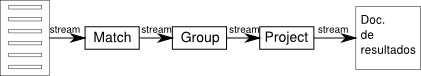
\includegraphics{aggregationFramework.png}

Para poder realizar operaciones en paralelo hay que usar ``Map Reduce'', el resto son secuenciales.


\section{Operadores}
\label{contents/aggregationFramework:operadores}\begin{itemize}
\item {} 
\textbf{\$match}. igual a queries (find(\{\}))

\item {} 
\textbf{\$project}. como las proyecciones del find pero le podemos añadir mas elementos (sumas, divisiones...)

\item {} 
\textbf{\$group}. Parecido a db.coll.group() pero no es una función igual

\item {} 
\textbf{\$unwind}. Explotar el array -\textgreater{} Dado un array de 3 elementos, generamos 3 elementos individuales.

\item {} 
\textbf{\$sort}. Parecido a trabajar con el cursor, pero trabajamos con el stream.

\item {} 
\textbf{\$limit}.

\item {} 
\textbf{\$skip}.

\item {} 
\textbf{\$out}. Escritura en fichero

\end{itemize}

\textbf{Limitaciones:}
\begin{itemize}
\item {} 
\textbf{Pipeline operator memory limits: 100MB - No se puede cambiar}.

\item {} 
Lo que podemos hacer es habilitar el uso en disco: \code{allowDiskUse: true}

\end{itemize}


\subsection{\$match.}
\label{contents/aggregationFramework:match}\begin{itemize}
\item {} 
Filtra documentos como un find.

\item {} 
No nos valen operaciones geoespaciales

\item {} 
No es válido tampoco el \$where

\end{itemize}

\textbf{El resultado de la operación no es un cursor (no es un array). Es un documento que contiene los resultados.}

\begin{Verbatim}[commandchars=\\\{\}]
\PYGZgt{} db.zips.aggregate([ \PYGZob{}\PYGZdl{}match: \PYGZob{}state : \PYGZdq{}AL\PYGZdq{} \PYGZcb{}\PYGZcb{}])

//Ejemplo encadenando. {}`{}`\PYGZdl{}city{}`{}` es el valor del campo
\PYGZgt{} db.zips.aggregate([ \PYGZob{}\PYGZdl{}match: \PYGZob{}state : \PYGZdq{}AL\PYGZdq{} \PYGZcb{}\PYGZcb{},
        \PYGZob{}\PYGZdl{}project: \PYGZob{}\PYGZus{}id:0, city: \PYGZob{}\PYGZdl{}toUpper: \PYGZdq{}\PYGZdl{}city\PYGZdq{} \PYGZcb{}\PYGZcb{}\PYGZcb{}])
\end{Verbatim}


\subsection{\$group}
\label{contents/aggregationFramework:group}
Plantilla para los siguientes documentos (por la agrupación)

\textbf{Cuidado, ya que se procesa toda la información en memoria}

Ejemplo: calcular la población total por estado:

\begin{Verbatim}[commandchars=\\\{\}]
\PYGZgt{} db.zips.aggregate(\PYGZob{}\PYGZdl{}group: \PYGZob{}\PYGZus{}id: \PYGZdq{}\PYGZdl{}state\PYGZdq{}, pop\PYGZus{}total: \PYGZob{}\PYGZdl{}sum: \PYGZdq{}\PYGZdl{}pop\PYGZdq{}\PYGZcb{}\PYGZcb{}\PYGZcb{},
        \PYGZob{}\PYGZdl{}sort : \PYGZob{}pop\PYGZus{}total : \PYGZhy{}1\PYGZcb{}\PYGZcb{})
\PYGZgt{} db.zips.aggregate(\PYGZob{}\PYGZdl{}group: \PYGZob{}\PYGZus{}id: \PYGZdq{}\PYGZdl{}state\PYGZdq{}, pop\PYGZus{}total: \PYGZob{}\PYGZdl{}sum: \PYGZdq{}\PYGZdl{}pop\PYGZdq{}\PYGZcb{}\PYGZcb{}\PYGZcb{},
        \PYGZob{}\PYGZdl{}sort : \PYGZob{}pop\PYGZus{}total : \PYGZhy{}1\PYGZcb{}\PYGZcb{}, \PYGZob{}\PYGZdl{}limit: 2\PYGZcb{})
\PYGZob{} \PYGZdq{}\PYGZus{}id\PYGZdq{} : \PYGZdq{}CA\PYGZdq{}, \PYGZdq{}pop\PYGZus{}total\PYGZdq{} : 29760021 \PYGZcb{}
\PYGZob{} \PYGZdq{}\PYGZus{}id\PYGZdq{} : \PYGZdq{}NY\PYGZdq{}, \PYGZdq{}pop\PYGZus{}total\PYGZdq{} : 17990455 \PYGZcb{}
\end{Verbatim}

Ejemplo: media de población de los estados.

\begin{Verbatim}[commandchars=\\\{\}]
\PYGZgt{} db.zips.aggregate(\PYGZob{}\PYGZdl{}group: \PYGZob{}\PYGZus{}id: \PYGZdq{}\PYGZdl{}state\PYGZdq{}, pop\PYGZus{}total: \PYGZob{}\PYGZdl{}sum: \PYGZdq{}\PYGZdl{}pop\PYGZdq{}\PYGZcb{}\PYGZcb{}\PYGZcb{},
        \PYGZob{}\PYGZdl{}group: \PYGZob{}\PYGZus{}id: \PYGZdq{}total\PYGZdq{}, avg: \PYGZob{}\PYGZdl{}avg: \PYGZdq{}\PYGZdl{}pop\PYGZus{}total\PYGZdq{}\PYGZcb{}\PYGZcb{}\PYGZcb{} )
\PYGZob{} \PYGZdq{}\PYGZus{}id\PYGZdq{} : \PYGZdq{}total\PYGZdq{}, \PYGZdq{}avg\PYGZdq{} : 4876664.176470588 \PYGZcb{}
\end{Verbatim}

Proyecciones encadenadas:

\begin{Verbatim}[commandchars=\\\{\}]
\PYGZgt{} db.zips.aggregate([ \PYGZob{}\PYGZdl{}group: \PYGZob{}\PYGZus{}id: \PYGZob{}state: \PYGZdq{}\PYGZdl{}state\PYGZdq{}, city: \PYGZdq{}\PYGZdl{}city\PYGZdq{}\PYGZcb{},
        pop\PYGZus{}total: \PYGZob{}\PYGZdl{}sum: \PYGZdq{}\PYGZdl{}pop\PYGZdq{} \PYGZcb{}\PYGZcb{}\PYGZcb{},
        \PYGZob{}\PYGZdl{}group: \PYGZob{}\PYGZus{}id: \PYGZdq{}\PYGZdl{}\PYGZus{}id.state\PYGZdq{}, pop\PYGZus{}media : \PYGZob{}\PYGZdl{}avg : \PYGZdq{}\PYGZdl{}pop\PYGZus{}total\PYGZdq{}\PYGZcb{}\PYGZcb{}\PYGZcb{},
        \PYGZob{}\PYGZdl{}sort : \PYGZob{}pop\PYGZus{}media : \PYGZhy{}1\PYGZcb{}\PYGZcb{}])
\end{Verbatim}


\subsection{\$project}
\label{contents/aggregationFramework:project}
Proyecta los campos realizando operaciones si es necesario


\subsection{\$unwind}
\label{contents/aggregationFramework:unwind}
Hace una explosión de los elementos de un array a elementos simples.

\textbf{Si el campo no es un array da un error}


\subsection{\$sort, \$limit, \$skip}
\label{contents/aggregationFramework:sort-limit-skip}
Funcionan igual que en las queries normales.

\textbf{Cuidado con el tema de memoria de nuevo}.


\subsection{\$out}
\label{contents/aggregationFramework:out}
Sería siempre la última fase y crearía una nueva colección en la BD.

\begin{Verbatim}[commandchars=\\\{\}]
\PYGZob{}\PYGZdl{}out: \PYGZdq{}media\PYGZus{}x\PYGZus{}states\PYGZdq{}\PYGZcb{}
\end{Verbatim}


\section{Sharding}
\label{contents/aggregationFramework:sharding}
En el framework de agregación, si hacemos un match, el uso va a ser el mismo que sin sharding (se hace un match local, se juntan y se devuelven). Con la proyección pasa lo mismo.

El problema son en las agrupaciones que realizan cálculos o se necesitan todos los documentos (group, sort). Que tienen que traer todos los datos al primary shard para realizar todos las operaciones.

Podemos mejorar el rendimiento con el orden de operaciones en los shards, de forma que limitemos los resultados:
\begin{quote}

-\textgreater{} match, project, group, sort, project...
\end{quote}

Si esto se nos queda corto (manejar una gran cantidad de operaciones para agregaciones),
habría que plantearse otras soluciones alternativa a Mongo.

La alternativa mas usada es Hadoop (existe connector mongo-hadoop). Y en cantidades mayores: mahout, Hive/Pig, spark/storm, ...

Mongo -\textgreater{} Hadoop -\textgreater{} Mahout, Hive...

Podemos ver un explain en agregación con \code{\{explain: true\}}:

\begin{Verbatim}[commandchars=\\\{\}]
\PYGZgt{} db.tweets.aggregate([ \PYGZob{}\PYGZdl{}match: \PYGZob{}\PYGZdq{}user.friends\PYGZus{}count\PYGZdq{}: \PYGZob{}\PYGZdl{}gt: 0\PYGZcb{}\PYGZcb{}\PYGZcb{},
        \PYGZob{}\PYGZdl{}match: \PYGZob{}\PYGZdq{}user.followers\PYGZus{}count\PYGZdq{}: \PYGZob{}\PYGZdl{}gt: 0\PYGZcb{}\PYGZcb{}\PYGZcb{},
        \PYGZob{}\PYGZdl{}project: \PYGZob{} \PYGZdq{}user.screen\PYGZus{}name\PYGZdq{}: 1,
            \PYGZdq{}user.friends\PYGZus{}count\PYGZdq{}: 1,
            \PYGZdq{}user.followers\PYGZus{}count\PYGZdq{}: 1,
            \PYGZus{}id: 0,
            ratio: \PYGZob{}\PYGZdl{}divide:[\PYGZdq{}\PYGZdl{}user.followers\PYGZus{}count\PYGZdq{}, \PYGZdq{}\PYGZdl{}user.friends\PYGZus{}count\PYGZdq{}]\PYGZcb{}\PYGZcb{}
        \PYGZcb{},
        \PYGZob{}\PYGZdl{}group:\PYGZob{}\PYGZus{}id: 1, avg: \PYGZob{}\PYGZdl{}avg: \PYGZdq{}\PYGZdl{}ratio\PYGZdq{}\PYGZcb{}\PYGZcb{}\PYGZcb{}
    ], \PYGZob{}explain: true\PYGZcb{} )
\end{Verbatim}


\section{MapReduce}
\label{contents/aggregationFramework:mapreduce}
\href{http://docs.mongodb.org/manual/tutorial/map-reduce/}{http://docs.mongodb.org/manual/tutorial/map-reduce/}

Se usaba inicialmente, cuando no había funciones de agregación

Con map reduce hay que ir haciendo por fases, no hay pipeline:

\textbf{Fase mapeo}: filtro, parseo, limpieza, proyección, split de texto... Esto produce unos valores K,V (clave, valor)

\textbf{Fase reducción}: operaciones de agregación: sumas, medias, ...

\begin{Verbatim}[commandchars=\\\{\}]
map = function() \PYGZob{}
    emit( this.user.name, \PYGZob{} \PYGZdq{}diggs\PYGZdq{}: this.diggs, \PYGZdq{}posts\PYGZdq{} : 1 \PYGZcb{} ) ;
\PYGZcb{}

reduce = function(key, values) \PYGZob{}
    var diggs = 0;
    var posts = 0;
    values.forEach(function(doc) \PYGZob{}
        diggs += doc.diggs;
        posts += doc.posts;
    \PYGZcb{} ) ;
    return \PYGZob{} \PYGZdq{}diggs\PYGZdq{} : diggs, \PYGZdq{}posts\PYGZdq{} : posts \PYGZcb{} ;
\PYGZcb{}

db.stories.mapReduce( map, reduce, \PYGZob{} \PYGZdq{}out\PYGZdq{} : \PYGZdq{}digg\PYGZus{}users\PYGZdq{} \PYGZcb{} ) ;
\end{Verbatim}

\begin{notice}{important}{Important:}\begin{enumerate}
\item {} 
Can be run on secondary nodes to keep from bogging down primary’s performance.

\item {} 
Can only at most 16MB of result.

\end{enumerate}
\end{notice}


\chapter{Certificación}
\label{contents/certificacion::doc}\label{contents/certificacion:certificacion}
Preguntas típicas de certificación:
\begin{itemize}
\item {} 
\textbf{WriteConcern y ReadPreferences sobre clientes o tablas}.

\item {} 
\textbf{¿Cómo mejorar el rendimiento de las escrituras?}. Con un WriteConcern de W=0 o menos

\item {} 
Sobre unas 10 preguntas van a ser sobre el framework de agregación.

\end{itemize}


\chapter{Anexo. Otros recursos}
\label{contents/recursos::doc}\label{contents/recursos:anexo-otros-recursos}\begin{itemize}
\item {} 
\href{http://info.mongodb.com/rs/mongodb/images/MongoDB-Performance-Best-Practices.pdf}{MongoDB-Performance-Best-Practices.pdf}

\item {} 
Ejemplos encontrados de examenes:
\begin{itemize}
\item {} 
\href{http://blog.cloudthat.in/sample-questions-for-mongodb-certified-dba-c100dba-exam/}{http://blog.cloudthat.in/sample-questions-for-mongodb-certified-dba-c100dba-exam/}

\item {} 
\href{http://blog.cloudthat.in/sample-questions-for-mongodb-certified-dba-c100dba-exam-part-ii/}{http://blog.cloudthat.in/sample-questions-for-mongodb-certified-dba-c100dba-exam-part-ii/}

\end{itemize}

\end{itemize}


\chapter{Anexo. Ejercicios / Ejemplos}
\label{contents/ejercicios::doc}\label{contents/ejercicios:anexo-ejercicios-ejemplos}
\textbf{cambiar en la BD de tweeter, los campos user.location = ``'' o null por N/S}

Antes del cambio

\begin{Verbatim}[commandchars=\\\{\}]
\PYGZgt{} db.tweets.find(\PYGZob{}\PYGZdl{}or : [\PYGZob{}\PYGZdq{}user.location\PYGZdq{}:\PYGZdq{}\PYGZdq{}\PYGZcb{}, \PYGZob{}\PYGZdq{}user.location\PYGZdq{}:null\PYGZcb{}]\PYGZcb{}).count()
10796
\end{Verbatim}

Update:

\begin{Verbatim}[commandchars=\\\{\}]
\PYGZgt{} db.tweets.update(\PYGZob{}\PYGZdl{}or : [\PYGZob{}\PYGZdq{}user.location\PYGZdq{}:\PYGZdq{}\PYGZdq{}\PYGZcb{}, \PYGZob{}\PYGZdq{}user.location\PYGZdq{}: null\PYGZcb{}]\PYGZcb{},
        \PYGZob{}\PYGZdl{}set: \PYGZob{}\PYGZdq{}user.location\PYGZdq{}:\PYGZdq{}N/S\PYGZdq{}\PYGZcb{}\PYGZcb{}, \PYGZob{}multi:true\PYGZcb{})
WriteResult(\PYGZob{} \PYGZdq{}nMatched\PYGZdq{} : 10796, \PYGZdq{}nUpserted\PYGZdq{} : 0, \PYGZdq{}nModified\PYGZdq{} : 10796 \PYGZcb{})
\PYGZgt{} db.tweets.find(\PYGZob{}\PYGZdq{}user.location\PYGZdq{}:\PYGZdq{}N/S\PYGZdq{}\PYGZcb{}).count()
10796
\end{Verbatim}

\textbf{actualizar el campo ``created\_at'' que es String a un tipo Date de BSON}

\begin{Verbatim}[commandchars=\\\{\}]
\PYGZgt{} var cur = db.tweets.find(\PYGZob{}\PYGZcb{},\PYGZob{}created\PYGZus{}at:1\PYGZcb{})
\PYGZgt{} cur.forEach(function(it) \PYGZob{}db.tweets.update(\PYGZob{}\PYGZus{}id: it.\PYGZus{}id\PYGZcb{},
        \PYGZob{}\PYGZdl{}set:\PYGZob{}created\PYGZus{}at: new Date(it.created\PYGZus{}at)\PYGZcb{}\PYGZcb{})\PYGZcb{})
\end{Verbatim}

\textbf{Todos aquellos usuarios que tengan dentro de entidades, menciones de usuarios. Y los 10 usuarios con mas menciones.}

\begin{Verbatim}[commandchars=\\\{\}]
\PYGZgt{} db.tweets.count(\PYGZob{}\PYGZdq{}entities.user\PYGZus{}mentions\PYGZdq{}: \PYGZob{}\PYGZdl{}not:\PYGZob{}\PYGZdl{}size:0\PYGZcb{}\PYGZcb{}\PYGZcb{})
27069

\PYGZgt{} var cursor = db.tweets.find(\PYGZob{}\PYGZdq{}entities.user\PYGZus{}mentions\PYGZdq{}:
        \PYGZob{}\PYGZdl{}not:\PYGZob{}\PYGZdl{}size:0\PYGZcb{}\PYGZcb{}\PYGZcb{},\PYGZob{}\PYGZdq{}entities.user\PYGZus{}mentions\PYGZdq{}:1\PYGZcb{})
\PYGZgt{} cursor.forEach(function(it) \PYGZob{}db.tweets.update(\PYGZob{}\PYGZus{}id: it.\PYGZus{}id\PYGZcb{},
        \PYGZob{}\PYGZdl{}set:\PYGZob{}\PYGZdq{}mentions\PYGZus{}count\PYGZdq{}:it.entities.user\PYGZus{}mentions.length\PYGZcb{}\PYGZcb{})\PYGZcb{})
\PYGZgt{} db.tweets.find(\PYGZob{}\PYGZcb{},\PYGZob{}\PYGZdq{}user.screen\PYGZus{}name\PYGZdq{}:1,\PYGZdq{}mentions\PYGZus{}count\PYGZdq{}:1\PYGZcb{}).sort(
        \PYGZob{}mentions\PYGZus{}count:\PYGZhy{}1\PYGZcb{}).limit(10)
\end{Verbatim}

\begin{notice}{tip}{Tip:}
hay que tener en cuenta que puede haber mas usuarios que los mostrados con el mismo número de menciones que el mínimo que mostramos. En nuestro caso hay 18 usuarios con 10 menciones.
\end{notice}

\textbf{Do a regular expression query for all users with screen names beginning with `a'. Verify that this uses an index}

\begin{Verbatim}[commandchars=\\\{\}]
\PYGZgt{} db.tweets.ensureIndex(\PYGZob{}\PYGZdq{}user.screen\PYGZus{}name\PYGZdq{}: 1\PYGZcb{})
\PYGZgt{} db.tweets.find(\PYGZob{}\PYGZdq{}user.screen\PYGZus{}name\PYGZdq{}: /\PYGZca{}a/\PYGZcb{},
        \PYGZob{}\PYGZdq{}user.screen\PYGZus{}name\PYGZdq{}:1, \PYGZus{}id: 0\PYGZcb{}).explain()
\end{Verbatim}

\textbf{Using the twitter collection, build a simple index on a user's friends count. Then build a separate compound index on both friends count and followers counts. Run a few queries against these fields using explain(), and notice which indexes the query optimizer uses}

\begin{Verbatim}[commandchars=\\\{\}]
\PYGZgt{} db.tweets.ensureIndex(\PYGZob{}\PYGZdq{}user.friends\PYGZus{}count\PYGZdq{}:1\PYGZcb{})
\PYGZgt{} db.tweets.ensureIndex(\PYGZob{}\PYGZdq{}user.friends\PYGZus{}count\PYGZdq{}:1, \PYGZdq{}user.followers\PYGZus{}count\PYGZdq{}:1\PYGZcb{})

\PYGZgt{} db.tweets.find(\PYGZob{}\PYGZcb{}).sort(\PYGZob{}\PYGZdq{}user.friends\PYGZus{}count\PYGZdq{}: \PYGZhy{}1\PYGZcb{}).explain()
\PYGZgt{} db.tweets.find(\PYGZob{}\PYGZcb{}).sort(\PYGZob{}\PYGZdq{}user.followers\PYGZus{}count\PYGZdq{}: \PYGZhy{}1\PYGZcb{}).explain() //ERROR
\PYGZgt{} db.tweets.find(\PYGZob{}\PYGZcb{}).sort(\PYGZob{}\PYGZdq{}user.friends\PYGZus{}count\PYGZdq{}:1,
        \PYGZdq{}user.followers\PYGZus{}count\PYGZdq{}: 1\PYGZcb{}).explain()
\end{Verbatim}


\section{Framework de agregación}
\label{contents/ejercicios:framework-de-agregacion}\begin{itemize}
\item {} 
By screen name who tweeted the most?

\begin{Verbatim}[commandchars=\\\{\}]
\PYGZgt{} db.tweets.aggregate( \PYGZob{}\PYGZdl{}group: \PYGZob{}\PYGZus{}id: \PYGZdq{}\PYGZdl{}user.screen\PYGZus{}name\PYGZdq{}, count: \PYGZob{}\PYGZdl{}sum: 1\PYGZcb{}\PYGZcb{}\PYGZcb{},
        \PYGZob{}\PYGZdl{}sort:\PYGZob{}count:\PYGZhy{}1\PYGZcb{}\PYGZcb{},\PYGZob{}\PYGZdl{}limit: 1\PYGZcb{} )
\PYGZob{} \PYGZdq{}\PYGZus{}id\PYGZdq{} : \PYGZdq{}behcolin\PYGZdq{}, \PYGZdq{}count\PYGZdq{} : 8 \PYGZcb{}
\end{Verbatim}

\item {} 
Who mentions the most other (unique) tweeters in their tweets? ...

\item {} 
Ignoring anyone with no friends or no followers:
\begin{enumerate}
\item {} 
Who has the highest Followers to Friends (follows) Ratio?

\begin{Verbatim}[commandchars=\\\{\}]
\PYGZgt{} db.tweets.aggregate(\PYGZob{}\PYGZdl{}match: \PYGZob{}\PYGZdq{}user.friends\PYGZus{}count\PYGZdq{}: \PYGZob{}\PYGZdl{}gt: 0\PYGZcb{}\PYGZcb{}\PYGZcb{},
        \PYGZob{}\PYGZdl{}match: \PYGZob{}\PYGZdq{}user.followers\PYGZus{}count\PYGZdq{}: \PYGZob{}\PYGZdl{}gt: 0\PYGZcb{}\PYGZcb{}\PYGZcb{},
        \PYGZob{}\PYGZdl{}project: \PYGZob{}\PYGZdq{}user.screen\PYGZus{}name\PYGZdq{}: 1,
            \PYGZdq{}user.friends\PYGZus{}count\PYGZdq{}: 1,
            \PYGZdq{}user.followers\PYGZus{}count\PYGZdq{}: 1,
            \PYGZus{}id: 0,
            ratio: \PYGZob{}\PYGZdl{}divide:[\PYGZdq{}\PYGZdl{}user.followers\PYGZus{}count\PYGZdq{},
                             \PYGZdq{}\PYGZdl{}user.friends\PYGZus{}count\PYGZdq{}]\PYGZcb{}
        \PYGZcb{}\PYGZcb{},
        \PYGZob{}\PYGZdl{}sort:\PYGZob{}ratio: \PYGZhy{}1\PYGZcb{}\PYGZcb{},
        \PYGZob{}\PYGZdl{}limit: 1\PYGZcb{})

\PYGZob{} \PYGZdq{}user\PYGZdq{} : \PYGZob{} \PYGZdq{}friends\PYGZus{}count\PYGZdq{} : 8, \PYGZdq{}screen\PYGZus{}name\PYGZdq{} : \PYGZdq{}Twitterrific\PYGZdq{},
        \PYGZdq{}followers\PYGZus{}count\PYGZdq{} : 153772 \PYGZcb{}, \PYGZdq{}ratio\PYGZdq{} : 19221.5 \PYGZcb{}
\end{Verbatim}

\item {} 
Who has the lowest?

\begin{Verbatim}[commandchars=\\\{\}]
\PYGZgt{} db.tweets.aggregate(\PYGZob{}\PYGZdl{}match: \PYGZob{}\PYGZdq{}user.friends\PYGZus{}count\PYGZdq{}: \PYGZob{}\PYGZdl{}gt: 0\PYGZcb{}\PYGZcb{}\PYGZcb{},
        \PYGZob{}\PYGZdl{}match: \PYGZob{}\PYGZdq{}user.followers\PYGZus{}count\PYGZdq{}: \PYGZob{}\PYGZdl{}gt: 0\PYGZcb{}\PYGZcb{}\PYGZcb{},
        \PYGZob{}\PYGZdl{}project: \PYGZob{}
            \PYGZdq{}user.screen\PYGZus{}name\PYGZdq{}: 1,
            \PYGZdq{}user.friends\PYGZus{}count\PYGZdq{}: 1,
            \PYGZdq{}user.followers\PYGZus{}count\PYGZdq{}: 1,
            \PYGZus{}id: 0,
            ratio: \PYGZob{}\PYGZdl{}divide:[\PYGZdq{}\PYGZdl{}user.followers\PYGZus{}count\PYGZdq{},
                             \PYGZdq{}\PYGZdl{}user.friends\PYGZus{}count\PYGZdq{}]\PYGZcb{}
        \PYGZcb{}\PYGZcb{},
        \PYGZob{}\PYGZdl{}sort:\PYGZob{}ratio: 1\PYGZcb{}\PYGZcb{},
        \PYGZob{}\PYGZdl{}limit: 1\PYGZcb{})

\PYGZob{} \PYGZdq{}user\PYGZdq{} : \PYGZob{} \PYGZdq{}friends\PYGZus{}count\PYGZdq{} : 121, \PYGZdq{}screen\PYGZus{}name\PYGZdq{} : \PYGZdq{}whaider2009\PYGZdq{},
        \PYGZdq{}followers\PYGZus{}count\PYGZdq{} : 1 \PYGZcb{}, \PYGZdq{}ratio\PYGZdq{} : 0.008264462809917356 \PYGZcb{}
\end{Verbatim}

\item {} 
What's the average?

\begin{Verbatim}[commandchars=\\\{\}]
\PYGZgt{} db.tweets.aggregate(\PYGZob{}\PYGZdl{}match: \PYGZob{}\PYGZdq{}user.friends\PYGZus{}count\PYGZdq{}: \PYGZob{}\PYGZdl{}gt: 0\PYGZcb{}\PYGZcb{}\PYGZcb{},
        \PYGZob{}\PYGZdl{}match: \PYGZob{}\PYGZdq{}user.followers\PYGZus{}count\PYGZdq{}: \PYGZob{}\PYGZdl{}gt: 0\PYGZcb{}\PYGZcb{}\PYGZcb{},
        \PYGZob{}\PYGZdl{}project: \PYGZob{}
            \PYGZdq{}user.screen\PYGZus{}name\PYGZdq{}: 1,
            \PYGZdq{}user.friends\PYGZus{}count\PYGZdq{}: 1,
            \PYGZdq{}user.followers\PYGZus{}count\PYGZdq{}: 1,
            \PYGZus{}id: 0,
            ratio: \PYGZob{}\PYGZdl{}divide:[\PYGZdq{}\PYGZdl{}user.followers\PYGZus{}count\PYGZdq{},
                             \PYGZdq{}\PYGZdl{}user.friends\PYGZus{}count\PYGZdq{}]\PYGZcb{}
            \PYGZcb{}\PYGZcb{},
            \PYGZob{}\PYGZdl{}group:\PYGZob{}\PYGZus{}id: 1, avg: \PYGZob{}\PYGZdl{}avg: \PYGZdq{}\PYGZdl{}ratio\PYGZdq{}\PYGZcb{}\PYGZcb{}\PYGZcb{})

\PYGZob{} \PYGZdq{}\PYGZus{}id\PYGZdq{} : 1, \PYGZdq{}avg\PYGZdq{} : 8.044204413696619 \PYGZcb{}
\end{Verbatim}

\item {} 
Who is closest to the average? ...

\end{enumerate}

\item {} 
Sacar de forma ordenada decreciente la diferencia entre followers
y friends (mas followers que friends) \textless{}- \textbf{Asegurar un índice!!}

\begin{Verbatim}[commandchars=\\\{\}]
\PYGZgt{} db.tweets.aggregate(\PYGZob{}\PYGZdl{}match: \PYGZob{}\PYGZdq{}user.friends\PYGZus{}count\PYGZdq{}: \PYGZob{}\PYGZdl{}gt: 0\PYGZcb{}\PYGZcb{}\PYGZcb{},
        \PYGZob{}\PYGZdl{}match: \PYGZob{}\PYGZdq{}user.followers\PYGZus{}count\PYGZdq{}: \PYGZob{}\PYGZdl{}gt: 0\PYGZcb{}\PYGZcb{}\PYGZcb{},
        \PYGZob{}\PYGZdl{}project: \PYGZob{}
            \PYGZdq{}user.screen\PYGZus{}name\PYGZdq{}: 1,
            \PYGZdq{}user.friends\PYGZus{}count\PYGZdq{}: 1,
            \PYGZdq{}user.followers\PYGZus{}count\PYGZdq{}: 1,
            \PYGZus{}id: 0,
            ratio: \PYGZob{}\PYGZdl{}divide:[\PYGZdq{}\PYGZdl{}user.followers\PYGZus{}count\PYGZdq{}, \PYGZdq{}\PYGZdl{}user.friends\PYGZus{}count\PYGZdq{}]\PYGZcb{},
            diferencia: \PYGZob{}\PYGZdl{}subtract: [
                \PYGZdq{}\PYGZdl{}user.followers\PYGZus{}count\PYGZdq{},\PYGZdq{}\PYGZdl{}user.friends\PYGZus{}count\PYGZdq{}]\PYGZcb{}
        \PYGZcb{}\PYGZcb{},
        \PYGZob{}\PYGZdl{}sort:\PYGZob{}ratio: \PYGZhy{}1\PYGZcb{}\PYGZcb{},
        \PYGZob{}\PYGZdl{}limit: 10\PYGZcb{})

\PYGZob{} \PYGZdq{}user\PYGZdq{} : \PYGZob{} \PYGZdq{}friends\PYGZus{}count\PYGZdq{} : 8, \PYGZdq{}screen\PYGZus{}name\PYGZdq{} : \PYGZdq{}Twitterrific\PYGZdq{},
        \PYGZdq{}followers\PYGZus{}count\PYGZdq{} : 153772 \PYGZcb{}, \PYGZdq{}ratio\PYGZdq{} : 19221.5,
        \PYGZdq{}diferencia\PYGZdq{} : 153764 \PYGZcb{}
\PYGZob{} \PYGZdq{}user\PYGZdq{} : \PYGZob{} \PYGZdq{}friends\PYGZus{}count\PYGZdq{} : 2, \PYGZdq{}screen\PYGZus{}name\PYGZdq{} : \PYGZdq{}steve\PYGZus{}berra\PYGZdq{},
        \PYGZdq{}followers\PYGZus{}count\PYGZdq{} : 34248 \PYGZcb{}, \PYGZdq{}ratio\PYGZdq{} : 17124,
        \PYGZdq{}diferencia\PYGZdq{} : 34246 \PYGZcb{}
\PYGZob{} \PYGZdq{}user\PYGZdq{} : \PYGZob{} \PYGZdq{}friends\PYGZus{}count\PYGZdq{} : 1, \PYGZdq{}screen\PYGZus{}name\PYGZdq{} : \PYGZdq{}2dopeboyz\PYGZdq{},
        \PYGZdq{}followers\PYGZus{}count\PYGZdq{} : 16847 \PYGZcb{}, \PYGZdq{}ratio\PYGZdq{} : 16847,
        \PYGZdq{}diferencia\PYGZdq{} : 16846 \PYGZcb{}
\PYGZob{} \PYGZdq{}user\PYGZdq{} : \PYGZob{} \PYGZdq{}friends\PYGZus{}count\PYGZdq{} : 9, \PYGZdq{}screen\PYGZus{}name\PYGZdq{} : \PYGZdq{}backstreetboys\PYGZdq{},
        \PYGZdq{}followers\PYGZus{}count\PYGZdq{} : 125048 \PYGZcb{}, \PYGZdq{}ratio\PYGZdq{} : 13894.222222222223,
        \PYGZdq{}diferencia\PYGZdq{} : 125039 \PYGZcb{}
\PYGZob{} \PYGZdq{}user\PYGZdq{} : \PYGZob{} \PYGZdq{}friends\PYGZus{}count\PYGZdq{} : 3, \PYGZdq{}screen\PYGZus{}name\PYGZdq{} : \PYGZdq{}tedouumdado\PYGZdq{},
        \PYGZdq{}followers\PYGZus{}count\PYGZdq{} : 39467 \PYGZcb{}, \PYGZdq{}ratio\PYGZdq{} : 13155.666666666666,
        \PYGZdq{}diferencia\PYGZdq{} : 39464 \PYGZcb{}
\PYGZob{} \PYGZdq{}user\PYGZdq{} : \PYGZob{} \PYGZdq{}friends\PYGZus{}count\PYGZdq{} : 1, \PYGZdq{}screen\PYGZus{}name\PYGZdq{} : \PYGZdq{}3in1of2\PYGZdq{},
        \PYGZdq{}followers\PYGZus{}count\PYGZdq{} : 10962 \PYGZcb{}, \PYGZdq{}ratio\PYGZdq{} : 10962,
        \PYGZdq{}diferencia\PYGZdq{} : 10961 \PYGZcb{}
\PYGZob{} \PYGZdq{}user\PYGZdq{} : \PYGZob{} \PYGZdq{}friends\PYGZus{}count\PYGZdq{} : 1, \PYGZdq{}screen\PYGZus{}name\PYGZdq{} : \PYGZdq{}craigslistjobs\PYGZdq{},
        \PYGZdq{}followers\PYGZus{}count\PYGZdq{} : 8742 \PYGZcb{}, \PYGZdq{}ratio\PYGZdq{} : 8742,
        \PYGZdq{}diferencia\PYGZdq{} : 8741 \PYGZcb{}
\PYGZob{} \PYGZdq{}user\PYGZdq{} : \PYGZob{} \PYGZdq{}friends\PYGZus{}count\PYGZdq{} : 1, \PYGZdq{}screen\PYGZus{}name\PYGZdq{} : \PYGZdq{}LaJornada\PYGZdq{},
        \PYGZdq{}followers\PYGZus{}count\PYGZdq{} : 8720 \PYGZcb{}, \PYGZdq{}ratio\PYGZdq{} : 8720,
        \PYGZdq{}diferencia\PYGZdq{} : 8719 \PYGZcb{}
\PYGZob{} \PYGZdq{}user\PYGZdq{} : \PYGZob{} \PYGZdq{}friends\PYGZus{}count\PYGZdq{} : 6, \PYGZdq{}screen\PYGZus{}name\PYGZdq{} : \PYGZdq{}trampos\PYGZdq{},
        \PYGZdq{}followers\PYGZus{}count\PYGZdq{} : 35508 \PYGZcb{}, \PYGZdq{}ratio\PYGZdq{} : 5918,
        \PYGZdq{}diferencia\PYGZdq{} : 35502 \PYGZcb{}
\PYGZob{} \PYGZdq{}user\PYGZdq{} : \PYGZob{} \PYGZdq{}friends\PYGZus{}count\PYGZdq{} : 1, \PYGZdq{}screen\PYGZus{}name\PYGZdq{} : \PYGZdq{}StyleCareers\PYGZdq{},
        \PYGZdq{}followers\PYGZus{}count\PYGZdq{} : 3661 \PYGZcb{}, \PYGZdq{}ratio\PYGZdq{} : 3661,
        \PYGZdq{}diferencia\PYGZdq{} : 3660 \PYGZcb{}
\end{Verbatim}

\item {} 
Obtener una colección tipo:

\begin{Verbatim}[commandchars=\\\{\}]
\PYG{p}{\PYGZob{}}\PYG{n}{\PYGZus{}id}\PYG{p}{:} \PYG{n}{hashtag}\PYG{p}{,} \PYG{n}{tweets}\PYG{p}{:} \PYG{p}{[} \PYG{p}{\PYGZob{}}\PYG{n+nb}{id}\PYG{p}{:} \PYG{l+s}{\PYGZdq{}}\PYG{l+s}{\PYGZdq{}}\PYG{p}{,} \PYG{n}{text}\PYG{p}{:} \PYG{l+s}{\PYGZdq{}}\PYG{l+s}{\PYGZdq{}}\PYG{p}{,} \PYG{n}{screen\PYGZus{}name}\PYG{p}{:} \PYG{l+s}{\PYGZdq{}}\PYG{l+s}{\PYGZdq{}}\PYG{p}{\PYGZcb{}}\PYG{p}{,} \PYG{o}{.}\PYG{o}{.}\PYG{o}{.}\PYG{p}{]}\PYG{p}{\PYGZcb{}}
\end{Verbatim}

Es decir, tag y los tweets relacionados con el tweet

Con push:

\begin{Verbatim}[commandchars=\\\{\}]
\PYGZgt{} db.tweets.aggregate( \PYGZob{}\PYGZdl{}match: \PYGZob{}\PYGZdq{}entities.hashtags\PYGZdq{}: \PYGZob{}\PYGZdl{}not: \PYGZob{}\PYGZdl{}size: 0\PYGZcb{} \PYGZcb{} \PYGZcb{}\PYGZcb{},
        \PYGZob{}\PYGZdl{}project: \PYGZob{}
            \PYGZus{}id: 0,
            id:1,
            text: 1,
            \PYGZdq{}entities.hashtags\PYGZdq{}: 1,
            \PYGZdq{}user.screen\PYGZus{}name\PYGZdq{}:1\PYGZcb{}\PYGZcb{},
        \PYGZob{}\PYGZdl{}unwind:\PYGZdq{}\PYGZdl{}entities.hashtags\PYGZdq{}\PYGZcb{},
        \PYGZob{}\PYGZdl{}group:\PYGZob{}
            \PYGZus{}id: \PYGZdq{}\PYGZdl{}entities.hashtags.text\PYGZdq{},
            tweets: \PYGZob{}\PYGZdl{}push: \PYGZob{}
                        id: \PYGZdq{}\PYGZdl{}id\PYGZdq{},
                        text: \PYGZdq{}\PYGZdl{}text\PYGZdq{},
                        screen\PYGZus{}name: \PYGZdq{}\PYGZdl{}user.screen\PYGZus{}name\PYGZdq{}\PYGZcb{}\PYGZcb{}
        \PYGZcb{}\PYGZcb{}, ,
        \PYGZob{}\PYGZdl{}out: \PYGZdq{}hashtags\PYGZus{}tweets\PYGZdq{}\PYGZcb{})
\end{Verbatim}

Con addToSet (si no existe lo crea como array, si existe como array lo añade, \textbf{si existe y no es un array da un error}):

\begin{Verbatim}[commandchars=\\\{\}]
\PYGZgt{} db.tweets.aggregate( \PYGZob{}\PYGZdl{}match: \PYGZob{}\PYGZdq{}entities.hashtags\PYGZdq{}: \PYGZob{}\PYGZdl{}not: \PYGZob{}\PYGZdl{}size: 0\PYGZcb{} \PYGZcb{} \PYGZcb{}\PYGZcb{},
        \PYGZob{}\PYGZdl{}project: \PYGZob{}
            \PYGZus{}id: 0,
            id:1,
            text: 1,
            \PYGZdq{}entities.hashtags\PYGZdq{}: 1,
            \PYGZdq{}user.screen\PYGZus{}name\PYGZdq{}:1\PYGZcb{}\PYGZcb{},
        \PYGZob{}\PYGZdl{}unwind:\PYGZdq{}\PYGZdl{}entities.hashtags\PYGZdq{}\PYGZcb{},
        \PYGZob{}\PYGZdl{}group:\PYGZob{}
            \PYGZus{}id: \PYGZdq{}\PYGZdl{}entities.hashtags.text\PYGZdq{},
            tweets: \PYGZob{}\PYGZdl{}addToSet: \PYGZob{}
                        id: \PYGZdq{}\PYGZdl{}id\PYGZdq{},
                        text: \PYGZdq{}\PYGZdl{}text\PYGZdq{},
                        screen\PYGZus{}name: \PYGZdq{}\PYGZdl{}user.screen\PYGZus{}name\PYGZdq{}\PYGZcb{}\PYGZcb{}
        \PYGZcb{}\PYGZcb{},
        \PYGZob{}\PYGZdl{}out: \PYGZdq{}hashtags\PYGZus{}tweets\PYGZdq{}\PYGZcb{}
    ).pretty()
\end{Verbatim}

\end{itemize}


\chapter{Anexo. Ejemplos de despliegues en la misma máquina}
\label{contents/ejemplosDesplieguesLocal:anexo-ejemplos-de-despliegues-en-la-misma-maquina}\label{contents/ejemplosDesplieguesLocal::doc}
Ejemplos con máquinas vagrant. Usan el directorio \code{/home/vagrant/mongodata} para almacenar los ficheros de datos.

Los ejemplos de linea de comandos pueden ser pasados a ficheros de configuración con el antiguo formato.

Para lanzar los demonios usando los ficheros de configuración (YAML o antiguo formato) usar los comandos \code{-f} ó \code{-{-}config}.

Estos despliegues crearán todos los demonios en la misma máquina usando distintos puertos


\section{Linea de comandos}
\label{contents/ejemplosDesplieguesLocal:linea-de-comandos}

\subsection{Standalone}
\label{contents/ejemplosDesplieguesLocal:standalone}
\begin{Verbatim}[commandchars=\\\{\}]
mkdir \PYGZhy{}p /home/vagrant/mongodata/standalone/db

mongod \PYGZhy{}\PYGZhy{}dbpath=/home/vagrant/mongodata/standalone/db \PYGZhy{}\PYGZhy{}journal \PYGZbs{}
    \PYGZhy{}\PYGZhy{}fork \PYGZhy{}\PYGZhy{}logpath=/home/vagrant/mongodata/standalone/db.log \PYGZhy{}\PYGZhy{}logappend

mongo
\end{Verbatim}


\subsection{Replica Set}
\label{contents/ejemplosDesplieguesLocal:replica-set}
\begin{Verbatim}[commandchars=\\\{\}]
mkdir \PYGZhy{}p /home/vagrant/mongodata/replicaSet/\PYGZob{}node1,node2,node3\PYGZcb{}/db

mongod \PYGZhy{}\PYGZhy{}dbpath=/home/vagrant/mongodata/replicaSet/node1/db \PYGZhy{}\PYGZhy{}journal \PYGZbs{}
    \PYGZhy{}\PYGZhy{}fork \PYGZhy{}\PYGZhy{}logpath=/home/vagrant/mongodata/replicaSet/node1/db.log \PYGZbs{}
    \PYGZhy{}\PYGZhy{}logappend \PYGZhy{}\PYGZhy{}replSet set0 \PYGZhy{}\PYGZhy{}port 28001
mongod \PYGZhy{}\PYGZhy{}dbpath=/home/vagrant/mongodata/replicaSet/node2/db \PYGZhy{}\PYGZhy{}journal \PYGZbs{}
    \PYGZhy{}\PYGZhy{}fork \PYGZhy{}\PYGZhy{}logpath=/home/vagrant/mongodata/replicaSet/node2/db.log \PYGZbs{}
    \PYGZhy{}\PYGZhy{}logappend \PYGZhy{}\PYGZhy{}replSet set0 \PYGZhy{}\PYGZhy{}port 28002
mongod \PYGZhy{}\PYGZhy{}dbpath=/home/vagrant/mongodata/replicaSet/node3/db \PYGZhy{}\PYGZhy{}journal \PYGZbs{}
    \PYGZhy{}\PYGZhy{}fork \PYGZhy{}\PYGZhy{}logpath=/home/vagrant/mongodata/replicaSet/node3/db.log \PYGZbs{}
    \PYGZhy{}\PYGZhy{}logappend \PYGZhy{}\PYGZhy{}replSet set0 \PYGZhy{}\PYGZhy{}port 28003

mongo \PYGZhy{}\PYGZhy{}port 28001
\end{Verbatim}

\textbf{Inicialización del replica set}

\begin{Verbatim}[commandchars=\\\{\}]
\PYG{n}{config} \PYG{o}{=} \PYG{p}{\PYGZob{}} \PYG{l+s}{\PYGZdq{}}\PYG{l+s}{\PYGZus{}id}\PYG{l+s}{\PYGZdq{}}\PYG{p}{:} \PYG{l+s}{\PYGZdq{}}\PYG{l+s}{set0}\PYG{l+s}{\PYGZdq{}}\PYG{p}{,} \PYG{l+s}{\PYGZdq{}}\PYG{l+s}{members}\PYG{l+s}{\PYGZdq{}} \PYG{p}{:} \PYG{p}{[}
    \PYG{p}{\PYGZob{}}\PYG{l+s}{\PYGZdq{}}\PYG{l+s}{\PYGZus{}id}\PYG{l+s}{\PYGZdq{}} \PYG{p}{:} \PYG{l+m+mi}{0}\PYG{p}{,} \PYG{l+s}{\PYGZdq{}}\PYG{l+s}{host}\PYG{l+s}{\PYGZdq{}} \PYG{p}{:} \PYG{l+s}{\PYGZdq{}}\PYG{l+s}{precise32:28001}\PYG{l+s}{\PYGZdq{}} \PYG{p}{\PYGZcb{}}\PYG{p}{,}
    \PYG{p}{\PYGZob{}}\PYG{l+s}{\PYGZdq{}}\PYG{l+s}{\PYGZus{}id}\PYG{l+s}{\PYGZdq{}} \PYG{p}{:} \PYG{l+m+mi}{1}\PYG{p}{,} \PYG{l+s}{\PYGZdq{}}\PYG{l+s}{host}\PYG{l+s}{\PYGZdq{}} \PYG{p}{:} \PYG{l+s}{\PYGZdq{}}\PYG{l+s}{precise32:28002}\PYG{l+s}{\PYGZdq{}} \PYG{p}{\PYGZcb{}}\PYG{p}{,}
    \PYG{p}{\PYGZob{}}\PYG{l+s}{\PYGZdq{}}\PYG{l+s}{\PYGZus{}id}\PYG{l+s}{\PYGZdq{}} \PYG{p}{:} \PYG{l+m+mi}{2}\PYG{p}{,} \PYG{l+s}{\PYGZdq{}}\PYG{l+s}{host}\PYG{l+s}{\PYGZdq{}} \PYG{p}{:} \PYG{l+s}{\PYGZdq{}}\PYG{l+s}{precise32:28003}\PYG{l+s}{\PYGZdq{}} \PYG{p}{\PYGZcb{}} \PYG{p}{]}
\PYG{p}{\PYGZcb{}}
\PYG{n}{rs}\PYG{o}{.}\PYG{n}{initiate}\PYG{p}{(}\PYG{n}{config}\PYG{p}{)}
\end{Verbatim}


\subsection{Shard}
\label{contents/ejemplosDesplieguesLocal:shard}
\begin{Verbatim}[commandchars=\\\{\}]
mkdir \PYGZhy{}p /home/vagrant/mongodata/shard/rs\PYGZob{}1,2\PYGZcb{}/node\PYGZob{}1,2,3\PYGZcb{}/db
mkdir \PYGZhy{}p /home/vagrant/mongodata/shard/config\PYGZus{}server\PYGZus{}\PYGZob{}1,2,3\PYGZcb{}

mongod \PYGZhy{}\PYGZhy{}dbpath=/home/vagrant/mongodata/shard/rs1/node1/db \PYGZhy{}\PYGZhy{}journal \PYGZbs{}
    \PYGZhy{}\PYGZhy{}fork \PYGZhy{}\PYGZhy{}logpath=/home/vagrant/mongodata/shard/rs1/node1/db.log \PYGZbs{}
    \PYGZhy{}\PYGZhy{}logappend \PYGZhy{}\PYGZhy{}replSet set1 \PYGZhy{}\PYGZhy{}port 28001 \PYGZhy{}\PYGZhy{}shardsvr
mongod \PYGZhy{}\PYGZhy{}dbpath=/home/vagrant/mongodata/shard/rs1/node2/db \PYGZhy{}\PYGZhy{}journal \PYGZbs{}
    \PYGZhy{}\PYGZhy{}fork \PYGZhy{}\PYGZhy{}logpath=/home/vagrant/mongodata/shard/rs1/node2/db.log \PYGZbs{}
    \PYGZhy{}\PYGZhy{}logappend \PYGZhy{}\PYGZhy{}replSet set1 \PYGZhy{}\PYGZhy{}port 28002 \PYGZhy{}\PYGZhy{}shardsvr
mongod \PYGZhy{}\PYGZhy{}dbpath=/home/vagrant/mongodata/shard/rs1/node3/db \PYGZhy{}\PYGZhy{}journal \PYGZbs{}
    \PYGZhy{}\PYGZhy{}fork \PYGZhy{}\PYGZhy{}logpath=/home/vagrant/mongodata/shard/rs1/node3/db.log \PYGZbs{}
    \PYGZhy{}\PYGZhy{}logappend \PYGZhy{}\PYGZhy{}replSet set1 \PYGZhy{}\PYGZhy{}port 28003 \PYGZhy{}\PYGZhy{}shardsvr

mongod \PYGZhy{}\PYGZhy{}dbpath=/home/vagrant/mongodata/shard/rs2/node1/db \PYGZhy{}\PYGZhy{}journal \PYGZbs{}
    \PYGZhy{}\PYGZhy{}fork \PYGZhy{}\PYGZhy{}logpath=/home/vagrant/mongodata/shard/rs2/node1/db.log \PYGZbs{}
    \PYGZhy{}\PYGZhy{}logappend \PYGZhy{}\PYGZhy{}replSet set2 \PYGZhy{}\PYGZhy{}port 28011 \PYGZhy{}\PYGZhy{}shardsvr
mongod \PYGZhy{}\PYGZhy{}dbpath=/home/vagrant/mongodata/shard/rs2/node2/db \PYGZhy{}\PYGZhy{}journal \PYGZbs{}
    \PYGZhy{}\PYGZhy{}fork \PYGZhy{}\PYGZhy{}logpath=/home/vagrant/mongodata/shard/rs2/node2/db.log \PYGZbs{}
    \PYGZhy{}\PYGZhy{}logappend \PYGZhy{}\PYGZhy{}replSet set2 \PYGZhy{}\PYGZhy{}port 28012 \PYGZhy{}\PYGZhy{}shardsvr
mongod \PYGZhy{}\PYGZhy{}dbpath=/home/vagrant/mongodata/shard/rs2/node3/db \PYGZhy{}\PYGZhy{}journal \PYGZbs{}
    \PYGZhy{}\PYGZhy{}fork \PYGZhy{}\PYGZhy{}logpath=/home/vagrant/mongodata/shard/rs2/node3/db.log \PYGZbs{}
    \PYGZhy{}\PYGZhy{}logappend \PYGZhy{}\PYGZhy{}replSet set2 \PYGZhy{}\PYGZhy{}port 28013 \PYGZhy{}\PYGZhy{}shardsvr

mongod \PYGZhy{}\PYGZhy{}dbpath=/home/vagrant/mongodata/shard/config\PYGZus{}server\PYGZus{}1 \PYGZhy{}\PYGZhy{}journal \PYGZbs{}
    \PYGZhy{}\PYGZhy{}fork \PYGZhy{}\PYGZhy{}logpath=/home/vagrant/mongodata/shard/config\PYGZus{}server\PYGZus{}1/mongod.log \PYGZbs{}
    \PYGZhy{}\PYGZhy{}logappend \PYGZhy{}\PYGZhy{}port 28101 \PYGZhy{}\PYGZhy{}configsvr
mongod \PYGZhy{}\PYGZhy{}dbpath=/home/vagrant/mongodata/shard/config\PYGZus{}server\PYGZus{}2 \PYGZhy{}\PYGZhy{}journal \PYGZbs{}
    \PYGZhy{}\PYGZhy{}fork \PYGZhy{}\PYGZhy{}logpath=/home/vagrant/mongodata/shard/config\PYGZus{}server\PYGZus{}2/mongod.log \PYGZbs{}
    \PYGZhy{}\PYGZhy{}logappend \PYGZhy{}\PYGZhy{}port 28102 \PYGZhy{}\PYGZhy{}configsvr
mongod \PYGZhy{}\PYGZhy{}dbpath=/home/vagrant/mongodata/shard/config\PYGZus{}server\PYGZus{}3 \PYGZhy{}\PYGZhy{}journal \PYGZbs{}
    \PYGZhy{}\PYGZhy{}fork \PYGZhy{}\PYGZhy{}logpath=/home/vagrant/mongodata/shard/config\PYGZus{}server\PYGZus{}3/mongod.log \PYGZbs{}
    \PYGZhy{}\PYGZhy{}logappend \PYGZhy{}\PYGZhy{}port 28103 \PYGZhy{}\PYGZhy{}configsvr

mongos \PYGZhy{}\PYGZhy{}configdb precise32:28101,precise32:28102,precise32:28103 \PYGZbs{}
    \PYGZhy{}\PYGZhy{}logpath=/home/vagrant/mongodata/shard/mongos.log \PYGZhy{}\PYGZhy{}logappend \PYGZbs{}
    \PYGZhy{}\PYGZhy{}fork \PYGZhy{}\PYGZhy{}port 28000
\end{Verbatim}

\textbf{Inicialización de los replica set}

\begin{Verbatim}[commandchars=\\\{\}]
\PYG{c}{\PYGZsh{} Conectar antes a un nodo del replica set (mongo \PYGZhy{}\PYGZhy{}port 28001)}
\PYG{n}{config} \PYG{o}{=} \PYG{p}{\PYGZob{}} \PYG{l+s}{\PYGZdq{}}\PYG{l+s}{\PYGZus{}id}\PYG{l+s}{\PYGZdq{}}\PYG{p}{:} \PYG{l+s}{\PYGZdq{}}\PYG{l+s}{set1}\PYG{l+s}{\PYGZdq{}}\PYG{p}{,} \PYG{l+s}{\PYGZdq{}}\PYG{l+s}{members}\PYG{l+s}{\PYGZdq{}} \PYG{p}{:} \PYG{p}{[}
    \PYG{p}{\PYGZob{}}\PYG{l+s}{\PYGZdq{}}\PYG{l+s}{\PYGZus{}id}\PYG{l+s}{\PYGZdq{}} \PYG{p}{:} \PYG{l+m+mi}{0}\PYG{p}{,} \PYG{l+s}{\PYGZdq{}}\PYG{l+s}{host}\PYG{l+s}{\PYGZdq{}} \PYG{p}{:} \PYG{l+s}{\PYGZdq{}}\PYG{l+s}{precise32:28001}\PYG{l+s}{\PYGZdq{}} \PYG{p}{\PYGZcb{}}\PYG{p}{,}
    \PYG{p}{\PYGZob{}}\PYG{l+s}{\PYGZdq{}}\PYG{l+s}{\PYGZus{}id}\PYG{l+s}{\PYGZdq{}} \PYG{p}{:} \PYG{l+m+mi}{1}\PYG{p}{,} \PYG{l+s}{\PYGZdq{}}\PYG{l+s}{host}\PYG{l+s}{\PYGZdq{}} \PYG{p}{:} \PYG{l+s}{\PYGZdq{}}\PYG{l+s}{precise32:28002}\PYG{l+s}{\PYGZdq{}} \PYG{p}{\PYGZcb{}}\PYG{p}{,}
    \PYG{p}{\PYGZob{}}\PYG{l+s}{\PYGZdq{}}\PYG{l+s}{\PYGZus{}id}\PYG{l+s}{\PYGZdq{}} \PYG{p}{:} \PYG{l+m+mi}{2}\PYG{p}{,} \PYG{l+s}{\PYGZdq{}}\PYG{l+s}{host}\PYG{l+s}{\PYGZdq{}} \PYG{p}{:} \PYG{l+s}{\PYGZdq{}}\PYG{l+s}{precise32:28003}\PYG{l+s}{\PYGZdq{}} \PYG{p}{\PYGZcb{}} \PYG{p}{]}
\PYG{p}{\PYGZcb{}}
\PYG{n}{rs}\PYG{o}{.}\PYG{n}{initiate}\PYG{p}{(}\PYG{n}{config}\PYG{p}{)}

\PYG{c}{\PYGZsh{} Conectar antes a un nodo del replica set (mongo \PYGZhy{}\PYGZhy{}port 28011)}
\PYG{n}{config} \PYG{o}{=} \PYG{p}{\PYGZob{}} \PYG{l+s}{\PYGZdq{}}\PYG{l+s}{\PYGZus{}id}\PYG{l+s}{\PYGZdq{}}\PYG{p}{:} \PYG{l+s}{\PYGZdq{}}\PYG{l+s}{set2}\PYG{l+s}{\PYGZdq{}}\PYG{p}{,} \PYG{l+s}{\PYGZdq{}}\PYG{l+s}{members}\PYG{l+s}{\PYGZdq{}} \PYG{p}{:} \PYG{p}{[}
    \PYG{p}{\PYGZob{}}\PYG{l+s}{\PYGZdq{}}\PYG{l+s}{\PYGZus{}id}\PYG{l+s}{\PYGZdq{}} \PYG{p}{:} \PYG{l+m+mi}{0}\PYG{p}{,} \PYG{l+s}{\PYGZdq{}}\PYG{l+s}{host}\PYG{l+s}{\PYGZdq{}} \PYG{p}{:} \PYG{l+s}{\PYGZdq{}}\PYG{l+s}{precise32:28011}\PYG{l+s}{\PYGZdq{}} \PYG{p}{\PYGZcb{}}\PYG{p}{,}
    \PYG{p}{\PYGZob{}}\PYG{l+s}{\PYGZdq{}}\PYG{l+s}{\PYGZus{}id}\PYG{l+s}{\PYGZdq{}} \PYG{p}{:} \PYG{l+m+mi}{1}\PYG{p}{,} \PYG{l+s}{\PYGZdq{}}\PYG{l+s}{host}\PYG{l+s}{\PYGZdq{}} \PYG{p}{:} \PYG{l+s}{\PYGZdq{}}\PYG{l+s}{precise32:28012}\PYG{l+s}{\PYGZdq{}} \PYG{p}{\PYGZcb{}}\PYG{p}{,}
    \PYG{p}{\PYGZob{}}\PYG{l+s}{\PYGZdq{}}\PYG{l+s}{\PYGZus{}id}\PYG{l+s}{\PYGZdq{}} \PYG{p}{:} \PYG{l+m+mi}{2}\PYG{p}{,} \PYG{l+s}{\PYGZdq{}}\PYG{l+s}{host}\PYG{l+s}{\PYGZdq{}} \PYG{p}{:} \PYG{l+s}{\PYGZdq{}}\PYG{l+s}{precise32:28013}\PYG{l+s}{\PYGZdq{}} \PYG{p}{\PYGZcb{}} \PYG{p}{]}
\PYG{p}{\PYGZcb{}}
\PYG{n}{rs}\PYG{o}{.}\PYG{n}{initiate}\PYG{p}{(}\PYG{n}{config}\PYG{p}{)}
\end{Verbatim}

\textbf{Inicialización de los shard}

\begin{Verbatim}[commandchars=\\\{\}]
\PYG{c}{\PYGZsh{} Conectar antes a mongos (mongo \PYGZhy{}\PYGZhy{}port 28000)}
\PYG{n}{sh}\PYG{o}{.}\PYG{n}{addShard}\PYG{p}{(}\PYG{l+s}{\PYGZdq{}}\PYG{l+s}{set1/precise32:28001}\PYG{l+s}{\PYGZdq{}}\PYG{p}{)}
\PYG{n}{sh}\PYG{o}{.}\PYG{n}{addShard}\PYG{p}{(}\PYG{l+s}{\PYGZdq{}}\PYG{l+s}{set2/precise32:28011}\PYG{l+s}{\PYGZdq{}}\PYG{p}{)}
\end{Verbatim}

\textbf{Activando sharding en una base de datos y tabla}

\begin{Verbatim}[commandchars=\\\{\}]
\PYG{n}{sh}\PYG{o}{.}\PYG{n}{enableSharding}\PYG{p}{(}\PYG{l+s}{\PYGZdq{}}\PYG{l+s}{mydb}\PYG{l+s}{\PYGZdq{}}\PYG{p}{)}
\PYG{c}{\PYGZsh{}Se necesita un índice sobre la shard key si no es \PYGZus{}id}
\PYG{n}{db}\PYG{o}{.}\PYG{n}{testtb}\PYG{o}{.}\PYG{n}{ensureIndex}\PYG{p}{(}\PYG{p}{\PYGZob{}}\PYG{n}{dummy}\PYG{p}{:}\PYG{l+m+mi}{1}\PYG{p}{\PYGZcb{}}\PYG{p}{)}
\PYG{n}{sh}\PYG{o}{.}\PYG{n}{shardCollection}\PYG{p}{(}\PYG{l+s}{\PYGZdq{}}\PYG{l+s}{mydb.testtb}\PYG{l+s}{\PYGZdq{}}\PYG{p}{,} \PYG{p}{\PYGZob{}}\PYG{n}{dummy}\PYG{p}{:}\PYG{l+m+mi}{1}\PYG{p}{\PYGZcb{}}\PYG{p}{)}
\end{Verbatim}


\section{YAML}
\label{contents/ejemplosDesplieguesLocal:yaml}
Nuevo formato de configuración. Estos ficheros .yml son los ficheros equivalentes a los ejemplos anteriores.

Sustituyen el lanzamiento del demonio \code{mongod} para pasarle solo el fichero de configuración:

\begin{Verbatim}[commandchars=\\\{\}]
mongod \PYGZhy{}f configfile.yml
\end{Verbatim}


\subsection{Standalone}
\label{contents/ejemplosDesplieguesLocal:id1}
\begin{Verbatim}[commandchars=\\\{\}]
\PYG{l+lScalar+lScalarPlain}{systemLog}\PYG{p+pIndicator}{:}
  \PYG{l+lScalar+lScalarPlain}{destination}\PYG{p+pIndicator}{:} \PYG{l+lScalar+lScalarPlain}{file}
  \PYG{l+lScalar+lScalarPlain}{path}\PYG{p+pIndicator}{:} \PYG{l+lScalar+lScalarPlain}{/home/vagrant/mongodata/standalone/db.log}
  \PYG{l+lScalar+lScalarPlain}{logAppend}\PYG{p+pIndicator}{:} \PYG{l+lScalar+lScalarPlain}{true}
\PYG{l+lScalar+lScalarPlain}{processManagement}\PYG{p+pIndicator}{:}
  \PYG{l+lScalar+lScalarPlain}{fork}\PYG{p+pIndicator}{:} \PYG{l+lScalar+lScalarPlain}{true}
\PYG{l+lScalar+lScalarPlain}{storage}\PYG{p+pIndicator}{:}
  \PYG{l+lScalar+lScalarPlain}{dbPath}\PYG{p+pIndicator}{:} \PYG{l+lScalar+lScalarPlain}{/home/vagrant/mongodata/standalone/db}
  \PYG{l+lScalar+lScalarPlain}{journal}\PYG{p+pIndicator}{:}
    \PYG{l+lScalar+lScalarPlain}{enabled}\PYG{p+pIndicator}{:} \PYG{l+lScalar+lScalarPlain}{true}
\end{Verbatim}


\subsection{Replica Set}
\label{contents/ejemplosDesplieguesLocal:id2}
\begin{Verbatim}[commandchars=\\\{\}]
\PYG{c+c1}{\PYGZsh{} node1\PYGZus{}conf.yml file}
\PYG{l+lScalar+lScalarPlain}{systemLog}\PYG{p+pIndicator}{:}
  \PYG{l+lScalar+lScalarPlain}{destination}\PYG{p+pIndicator}{:} \PYG{l+lScalar+lScalarPlain}{file}
  \PYG{l+lScalar+lScalarPlain}{path}\PYG{p+pIndicator}{:} \PYG{l+lScalar+lScalarPlain}{/home/vagrant/mongodata/replicaSet/node1/db.log}
  \PYG{l+lScalar+lScalarPlain}{logAppend}\PYG{p+pIndicator}{:} \PYG{l+lScalar+lScalarPlain}{true}
\PYG{l+lScalar+lScalarPlain}{processManagement}\PYG{p+pIndicator}{:}
  \PYG{l+lScalar+lScalarPlain}{fork}\PYG{p+pIndicator}{:} \PYG{l+lScalar+lScalarPlain}{true}
\PYG{l+lScalar+lScalarPlain}{net}\PYG{p+pIndicator}{:}
  \PYG{l+lScalar+lScalarPlain}{port}\PYG{p+pIndicator}{:} \PYG{l+lScalar+lScalarPlain}{28001}
\PYG{l+lScalar+lScalarPlain}{storage}\PYG{p+pIndicator}{:}
  \PYG{l+lScalar+lScalarPlain}{dbPath}\PYG{p+pIndicator}{:} \PYG{l+lScalar+lScalarPlain}{/home/vagrant/mongodata/replicaSet/node1/db}
  \PYG{l+lScalar+lScalarPlain}{journal}\PYG{p+pIndicator}{:}
    \PYG{l+lScalar+lScalarPlain}{enabled}\PYG{p+pIndicator}{:} \PYG{l+lScalar+lScalarPlain}{true}
\PYG{l+lScalar+lScalarPlain}{replication}\PYG{p+pIndicator}{:}
  \PYG{l+lScalar+lScalarPlain}{replSetName}\PYG{p+pIndicator}{:} \PYG{l+lScalar+lScalarPlain}{set0}

\PYG{c+c1}{\PYGZsh{} node2\PYGZus{}conf.yml file}
\PYG{l+lScalar+lScalarPlain}{systemLog}\PYG{p+pIndicator}{:}
  \PYG{l+lScalar+lScalarPlain}{destination}\PYG{p+pIndicator}{:} \PYG{l+lScalar+lScalarPlain}{file}
  \PYG{l+lScalar+lScalarPlain}{path}\PYG{p+pIndicator}{:} \PYG{l+lScalar+lScalarPlain}{/home/vagrant/mongodata/replicaSet/node2/db.log}
  \PYG{l+lScalar+lScalarPlain}{logAppend}\PYG{p+pIndicator}{:} \PYG{l+lScalar+lScalarPlain}{true}
\PYG{l+lScalar+lScalarPlain}{processManagement}\PYG{p+pIndicator}{:}
  \PYG{l+lScalar+lScalarPlain}{fork}\PYG{p+pIndicator}{:} \PYG{l+lScalar+lScalarPlain}{true}
\PYG{l+lScalar+lScalarPlain}{net}\PYG{p+pIndicator}{:}
  \PYG{l+lScalar+lScalarPlain}{port}\PYG{p+pIndicator}{:} \PYG{l+lScalar+lScalarPlain}{28002}
\PYG{l+lScalar+lScalarPlain}{storage}\PYG{p+pIndicator}{:}
  \PYG{l+lScalar+lScalarPlain}{dbPath}\PYG{p+pIndicator}{:} \PYG{l+lScalar+lScalarPlain}{/home/vagrant/mongodata/replicaSet/node2/db}
  \PYG{l+lScalar+lScalarPlain}{journal}\PYG{p+pIndicator}{:}
    \PYG{l+lScalar+lScalarPlain}{enabled}\PYG{p+pIndicator}{:} \PYG{l+lScalar+lScalarPlain}{true}
\PYG{l+lScalar+lScalarPlain}{replication}\PYG{p+pIndicator}{:}
  \PYG{l+lScalar+lScalarPlain}{replSetName}\PYG{p+pIndicator}{:} \PYG{l+lScalar+lScalarPlain}{set0}

\PYG{c+c1}{\PYGZsh{} node3\PYGZus{}conf.yml file}
\PYG{l+lScalar+lScalarPlain}{systemLog}\PYG{p+pIndicator}{:}
  \PYG{l+lScalar+lScalarPlain}{destination}\PYG{p+pIndicator}{:} \PYG{l+lScalar+lScalarPlain}{file}
  \PYG{l+lScalar+lScalarPlain}{path}\PYG{p+pIndicator}{:} \PYG{l+lScalar+lScalarPlain}{/home/vagrant/mongodata/replicaSet/node3/db.log}
  \PYG{l+lScalar+lScalarPlain}{logAppend}\PYG{p+pIndicator}{:} \PYG{l+lScalar+lScalarPlain}{true}
\PYG{l+lScalar+lScalarPlain}{processManagement}\PYG{p+pIndicator}{:}
  \PYG{l+lScalar+lScalarPlain}{fork}\PYG{p+pIndicator}{:} \PYG{l+lScalar+lScalarPlain}{true}
\PYG{l+lScalar+lScalarPlain}{net}\PYG{p+pIndicator}{:}
  \PYG{l+lScalar+lScalarPlain}{port}\PYG{p+pIndicator}{:} \PYG{l+lScalar+lScalarPlain}{28003}
\PYG{l+lScalar+lScalarPlain}{storage}\PYG{p+pIndicator}{:}
  \PYG{l+lScalar+lScalarPlain}{dbPath}\PYG{p+pIndicator}{:} \PYG{l+lScalar+lScalarPlain}{/home/vagrant/mongodata/replicaSet/node3/db}
  \PYG{l+lScalar+lScalarPlain}{journal}\PYG{p+pIndicator}{:}
    \PYG{l+lScalar+lScalarPlain}{enabled}\PYG{p+pIndicator}{:} \PYG{l+lScalar+lScalarPlain}{true}
\PYG{l+lScalar+lScalarPlain}{replication}\PYG{p+pIndicator}{:}
  \PYG{l+lScalar+lScalarPlain}{replSetName}\PYG{p+pIndicator}{:} \PYG{l+lScalar+lScalarPlain}{set0}
\end{Verbatim}


\subsection{Shard}
\label{contents/ejemplosDesplieguesLocal:id3}
\begin{Verbatim}[commandchars=\\\{\}]
\PYG{c+c1}{\PYGZsh{}rs1\PYGZus{}node1\PYGZus{}conf.yml}
\PYG{l+lScalar+lScalarPlain}{systemLog}\PYG{p+pIndicator}{:}
  \PYG{l+lScalar+lScalarPlain}{destination}\PYG{p+pIndicator}{:} \PYG{l+lScalar+lScalarPlain}{file}
  \PYG{l+lScalar+lScalarPlain}{path}\PYG{p+pIndicator}{:} \PYG{l+lScalar+lScalarPlain}{/home/vagrant/mongodata/shard/rs1/node1/db.log}
  \PYG{l+lScalar+lScalarPlain}{logAppend}\PYG{p+pIndicator}{:} \PYG{l+lScalar+lScalarPlain}{true}
\PYG{l+lScalar+lScalarPlain}{processManagement.fork}\PYG{p+pIndicator}{:} \PYG{l+lScalar+lScalarPlain}{true}
\PYG{l+lScalar+lScalarPlain}{net.port}\PYG{p+pIndicator}{:} \PYG{l+lScalar+lScalarPlain}{28001}
\PYG{l+lScalar+lScalarPlain}{storage}\PYG{p+pIndicator}{:}
  \PYG{l+lScalar+lScalarPlain}{dbPath}\PYG{p+pIndicator}{:} \PYG{l+lScalar+lScalarPlain}{/home/vagrant/mongodata/shard/rs1/node1/db}
  \PYG{l+lScalar+lScalarPlain}{journal.enabled}\PYG{p+pIndicator}{:} \PYG{l+lScalar+lScalarPlain}{true}
\PYG{l+lScalar+lScalarPlain}{replication.replSetName}\PYG{p+pIndicator}{:} \PYG{l+lScalar+lScalarPlain}{set1}
\PYG{l+lScalar+lScalarPlain}{sharding.clusterRole}\PYG{p+pIndicator}{:} \PYG{l+lScalar+lScalarPlain}{shardsvr}

\PYG{c+c1}{\PYGZsh{}... (Similar en el resto de nodos del mismo replica set 1)}

\PYG{c+c1}{\PYGZsh{}rs2\PYGZus{}node1\PYGZus{}conf.yml}
\PYG{l+lScalar+lScalarPlain}{systemLog}\PYG{p+pIndicator}{:}
  \PYG{l+lScalar+lScalarPlain}{destination}\PYG{p+pIndicator}{:} \PYG{l+lScalar+lScalarPlain}{file}
  \PYG{l+lScalar+lScalarPlain}{path}\PYG{p+pIndicator}{:} \PYG{l+lScalar+lScalarPlain}{/home/vagrant/mongodata/shard/rs2/node1/db.log}
  \PYG{l+lScalar+lScalarPlain}{logAppend}\PYG{p+pIndicator}{:} \PYG{l+lScalar+lScalarPlain}{true}
\PYG{l+lScalar+lScalarPlain}{processManagement.fork}\PYG{p+pIndicator}{:} \PYG{l+lScalar+lScalarPlain}{true}
\PYG{l+lScalar+lScalarPlain}{net.port}\PYG{p+pIndicator}{:} \PYG{l+lScalar+lScalarPlain}{28011}
\PYG{l+lScalar+lScalarPlain}{storage}\PYG{p+pIndicator}{:}
  \PYG{l+lScalar+lScalarPlain}{dbPath}\PYG{p+pIndicator}{:} \PYG{l+lScalar+lScalarPlain}{/home/vagrant/mongodata/shard/rs2/node1/db}
  \PYG{l+lScalar+lScalarPlain}{preallocDataFiles}\PYG{p+pIndicator}{:} \PYG{l+lScalar+lScalarPlain}{false}
  \PYG{l+lScalar+lScalarPlain}{smallFiles}\PYG{p+pIndicator}{:} \PYG{l+lScalar+lScalarPlain}{true}
  \PYG{l+lScalar+lScalarPlain}{journal.enabled}\PYG{p+pIndicator}{:} \PYG{l+lScalar+lScalarPlain}{true}
\PYG{l+lScalar+lScalarPlain}{replication.replSetName}\PYG{p+pIndicator}{:} \PYG{l+lScalar+lScalarPlain}{set2}
\PYG{l+lScalar+lScalarPlain}{sharding.clusterRole}\PYG{p+pIndicator}{:} \PYG{l+lScalar+lScalarPlain}{shardsvr}

\PYG{c+c1}{\PYGZsh{}... (Similar en el resto de nodos del mismo replica set 2)}

\PYG{c+c1}{\PYGZsh{}config\PYGZus{}server1\PYGZus{}conf.yml}
\PYG{l+lScalar+lScalarPlain}{systemLog}\PYG{p+pIndicator}{:}
  \PYG{l+lScalar+lScalarPlain}{destination}\PYG{p+pIndicator}{:} \PYG{l+lScalar+lScalarPlain}{file}
  \PYG{l+lScalar+lScalarPlain}{path}\PYG{p+pIndicator}{:} \PYG{l+lScalar+lScalarPlain}{/home/vagrant/mongodata/shard/config\PYGZus{}server\PYGZus{}1/mongod.log}
  \PYG{l+lScalar+lScalarPlain}{logAppend}\PYG{p+pIndicator}{:} \PYG{l+lScalar+lScalarPlain}{true}
\PYG{l+lScalar+lScalarPlain}{processManagement.fork}\PYG{p+pIndicator}{:} \PYG{l+lScalar+lScalarPlain}{true}
\PYG{l+lScalar+lScalarPlain}{net.port}\PYG{p+pIndicator}{:} \PYG{l+lScalar+lScalarPlain}{28101}
\PYG{l+lScalar+lScalarPlain}{storage}\PYG{p+pIndicator}{:}
  \PYG{l+lScalar+lScalarPlain}{dbPath}\PYG{p+pIndicator}{:} \PYG{l+lScalar+lScalarPlain}{/home/vagrant/mongodata/shard/config\PYGZus{}server\PYGZus{}1}
  \PYG{l+lScalar+lScalarPlain}{journal.enabled}\PYG{p+pIndicator}{:} \PYG{l+lScalar+lScalarPlain}{true}
\PYG{l+lScalar+lScalarPlain}{sharding.clusterRole}\PYG{p+pIndicator}{:} \PYG{l+lScalar+lScalarPlain}{configsvr}

\PYG{c+c1}{\PYGZsh{}... (Similar en el resto de nodos de config servers)}

\PYG{c+c1}{\PYGZsh{}mongos.yml}
\PYG{l+lScalar+lScalarPlain}{systemLog}\PYG{p+pIndicator}{:}
  \PYG{l+lScalar+lScalarPlain}{destination}\PYG{p+pIndicator}{:} \PYG{l+lScalar+lScalarPlain}{file}
  \PYG{l+lScalar+lScalarPlain}{path}\PYG{p+pIndicator}{:} \PYG{l+lScalar+lScalarPlain}{/home/vagrant/mongodata/shard/mongos.log}
  \PYG{l+lScalar+lScalarPlain}{logAppend}\PYG{p+pIndicator}{:} \PYG{l+lScalar+lScalarPlain}{true}
\PYG{l+lScalar+lScalarPlain}{processManagement.fork}\PYG{p+pIndicator}{:} \PYG{l+lScalar+lScalarPlain}{true}
\PYG{l+lScalar+lScalarPlain}{net.port}\PYG{p+pIndicator}{:} \PYG{l+lScalar+lScalarPlain}{28000}
\PYG{l+lScalar+lScalarPlain}{sharding.configDB}\PYG{p+pIndicator}{:} \PYG{l+s}{\PYGZdq{}}\PYG{l+s}{precise32:28101,precise32:28102,precise32:28103}\PYG{l+s}{\PYGZdq{}}
\end{Verbatim}


\chapter{Anexo. Ejemplos de despliegues en cluster}
\label{contents/ejemplosDesplieguesCluster::doc}\label{contents/ejemplosDesplieguesCluster:anexo-ejemplos-de-despliegues-en-cluster}
Ejemplo de despligue de un shard cluster con 2 shards y 3 nodos en cada replica set usando distintas máquinas.

\textbf{Información de la red}:
\begin{itemize}
\item {} 
3 máquinas:
\begin{itemize}
\item {} 
nodo1:              ip: ``192.168.50.101''

\item {} 
nodo2:              ip: ``192.168.50.102''

\item {} 
nodo3:              ip: ``192.168.50.103''

\end{itemize}

\item {} 
En cada máquina:
\begin{itemize}
\item {} 
shard\_server set1   port: 27001

\item {} 
shard\_server set2   port: 27002

\item {} 
configserver        port: 28000

\item {} 
mongos              port: 27017 (default port)

\end{itemize}

\end{itemize}

\textbf{Montaje de los replica set}:

Nos conectamos a un nodo de cada uno de los replica set e inicializamos los replica set.

\begin{Verbatim}[commandchars=\\\{\}]
\PYG{c}{\PYGZsh{} Replica set 1 (mongo \PYGZhy{}\PYGZhy{}host 192.168.50.101:27001)}
\PYG{n}{config} \PYG{o}{=} \PYG{p}{\PYGZob{}} \PYG{l+s}{\PYGZdq{}}\PYG{l+s}{\PYGZus{}id}\PYG{l+s}{\PYGZdq{}}\PYG{p}{:} \PYG{l+s}{\PYGZdq{}}\PYG{l+s}{set1}\PYG{l+s}{\PYGZdq{}}\PYG{p}{,} \PYG{l+s}{\PYGZdq{}}\PYG{l+s}{members}\PYG{l+s}{\PYGZdq{}} \PYG{p}{:} \PYG{p}{[}
    \PYG{p}{\PYGZob{}}\PYG{l+s}{\PYGZdq{}}\PYG{l+s}{\PYGZus{}id}\PYG{l+s}{\PYGZdq{}} \PYG{p}{:} \PYG{l+m+mi}{0}\PYG{p}{,} \PYG{l+s}{\PYGZdq{}}\PYG{l+s}{host}\PYG{l+s}{\PYGZdq{}} \PYG{p}{:} \PYG{l+s}{\PYGZdq{}}\PYG{l+s}{192.168.50.101:27001}\PYG{l+s}{\PYGZdq{}} \PYG{p}{\PYGZcb{}}\PYG{p}{,}
    \PYG{p}{\PYGZob{}}\PYG{l+s}{\PYGZdq{}}\PYG{l+s}{\PYGZus{}id}\PYG{l+s}{\PYGZdq{}} \PYG{p}{:} \PYG{l+m+mi}{1}\PYG{p}{,} \PYG{l+s}{\PYGZdq{}}\PYG{l+s}{host}\PYG{l+s}{\PYGZdq{}} \PYG{p}{:} \PYG{l+s}{\PYGZdq{}}\PYG{l+s}{192.168.50.102:27001}\PYG{l+s}{\PYGZdq{}} \PYG{p}{\PYGZcb{}}\PYG{p}{,}
    \PYG{p}{\PYGZob{}}\PYG{l+s}{\PYGZdq{}}\PYG{l+s}{\PYGZus{}id}\PYG{l+s}{\PYGZdq{}} \PYG{p}{:} \PYG{l+m+mi}{2}\PYG{p}{,} \PYG{l+s}{\PYGZdq{}}\PYG{l+s}{host}\PYG{l+s}{\PYGZdq{}} \PYG{p}{:} \PYG{l+s}{\PYGZdq{}}\PYG{l+s}{192.168.50.103:27001}\PYG{l+s}{\PYGZdq{}} \PYG{p}{\PYGZcb{}} \PYG{p}{]}
\PYG{p}{\PYGZcb{}}
\PYG{n}{rs}\PYG{o}{.}\PYG{n}{initiate}\PYG{p}{(}\PYG{n}{config}\PYG{p}{)}

\PYG{c}{\PYGZsh{} Replica set 2 (mongo \PYGZhy{}\PYGZhy{}host 192.168.50.101:27002)}
\PYG{n}{config} \PYG{o}{=} \PYG{p}{\PYGZob{}} \PYG{l+s}{\PYGZdq{}}\PYG{l+s}{\PYGZus{}id}\PYG{l+s}{\PYGZdq{}}\PYG{p}{:} \PYG{l+s}{\PYGZdq{}}\PYG{l+s}{set2}\PYG{l+s}{\PYGZdq{}}\PYG{p}{,} \PYG{l+s}{\PYGZdq{}}\PYG{l+s}{members}\PYG{l+s}{\PYGZdq{}} \PYG{p}{:} \PYG{p}{[}
    \PYG{p}{\PYGZob{}}\PYG{l+s}{\PYGZdq{}}\PYG{l+s}{\PYGZus{}id}\PYG{l+s}{\PYGZdq{}} \PYG{p}{:} \PYG{l+m+mi}{0}\PYG{p}{,} \PYG{l+s}{\PYGZdq{}}\PYG{l+s}{host}\PYG{l+s}{\PYGZdq{}} \PYG{p}{:} \PYG{l+s}{\PYGZdq{}}\PYG{l+s}{192.168.50.101:27002}\PYG{l+s}{\PYGZdq{}} \PYG{p}{\PYGZcb{}}\PYG{p}{,}
    \PYG{p}{\PYGZob{}}\PYG{l+s}{\PYGZdq{}}\PYG{l+s}{\PYGZus{}id}\PYG{l+s}{\PYGZdq{}} \PYG{p}{:} \PYG{l+m+mi}{1}\PYG{p}{,} \PYG{l+s}{\PYGZdq{}}\PYG{l+s}{host}\PYG{l+s}{\PYGZdq{}} \PYG{p}{:} \PYG{l+s}{\PYGZdq{}}\PYG{l+s}{192.168.50.102:27002}\PYG{l+s}{\PYGZdq{}} \PYG{p}{\PYGZcb{}}\PYG{p}{,}
    \PYG{p}{\PYGZob{}}\PYG{l+s}{\PYGZdq{}}\PYG{l+s}{\PYGZus{}id}\PYG{l+s}{\PYGZdq{}} \PYG{p}{:} \PYG{l+m+mi}{2}\PYG{p}{,} \PYG{l+s}{\PYGZdq{}}\PYG{l+s}{host}\PYG{l+s}{\PYGZdq{}} \PYG{p}{:} \PYG{l+s}{\PYGZdq{}}\PYG{l+s}{192.168.50.103:27002}\PYG{l+s}{\PYGZdq{}} \PYG{p}{\PYGZcb{}} \PYG{p}{]}
\PYG{p}{\PYGZcb{}}
\PYG{n}{rs}\PYG{o}{.}\PYG{n}{initiate}\PYG{p}{(}\PYG{n}{config}\PYG{p}{)}
\end{Verbatim}

Nos conectamos a mongos e inicializamos el shard.

\begin{Verbatim}[commandchars=\\\{\}]
\PYG{n}{sh}\PYG{o}{.}\PYG{n}{addShard}\PYG{p}{(}\PYG{l+s}{\PYGZdq{}}\PYG{l+s}{set1/192.168.50.101:27001}\PYG{l+s}{\PYGZdq{}}\PYG{p}{)}
\PYG{n}{sh}\PYG{o}{.}\PYG{n}{addShard}\PYG{p}{(}\PYG{l+s}{\PYGZdq{}}\PYG{l+s}{set2/192.168.50.101:27002}\PYG{l+s}{\PYGZdq{}}\PYG{p}{)}
\end{Verbatim}

\textbf{Plantillas de aprovisionamiento}:

\begin{Verbatim}[commandchars=\\\{\}]
\PYG{c+c1}{\PYGZsh{} mongo db shardsvr config}
\PYG{l+lScalar+lScalarPlain}{systemLog}\PYG{p+pIndicator}{:}
  \PYG{l+lScalar+lScalarPlain}{destination}\PYG{p+pIndicator}{:} \PYG{l+lScalar+lScalarPlain}{file}
  \PYG{l+lScalar+lScalarPlain}{path}\PYG{p+pIndicator}{:} \PYG{l+lScalar+lScalarPlain}{/home/vagrant/mongodata/\PYGZob{}\PYGZob{}set\PYGZus{}name\PYGZcb{}\PYGZcb{}/db.log}
  \PYG{l+lScalar+lScalarPlain}{logAppend}\PYG{p+pIndicator}{:} \PYG{l+lScalar+lScalarPlain}{true}
\PYG{l+lScalar+lScalarPlain}{processManagement}\PYG{p+pIndicator}{:}
  \PYG{l+lScalar+lScalarPlain}{fork}\PYG{p+pIndicator}{:} \PYG{l+lScalar+lScalarPlain}{true}
\PYG{l+lScalar+lScalarPlain}{net}\PYG{p+pIndicator}{:}
  \PYG{l+lScalar+lScalarPlain}{port}\PYG{p+pIndicator}{:} \PYG{p+pIndicator}{\PYGZob{}}\PYG{p+pIndicator}{\PYGZob{}}\PYG{n+nv}{port\PYGZus{}number}\PYG{p+pIndicator}{\PYGZcb{}}\PYG{p+pIndicator}{\PYGZcb{}}
\PYG{l+lScalar+lScalarPlain}{storage}\PYG{p+pIndicator}{:}
  \PYG{l+lScalar+lScalarPlain}{dbPath}\PYG{p+pIndicator}{:} \PYG{l+lScalar+lScalarPlain}{/home/vagrant/mongodata/\PYGZob{}\PYGZob{}set\PYGZus{}name\PYGZcb{}\PYGZcb{}}
  \PYG{l+lScalar+lScalarPlain}{journal}\PYG{p+pIndicator}{:}
    \PYG{l+lScalar+lScalarPlain}{enabled}\PYG{p+pIndicator}{:} \PYG{l+lScalar+lScalarPlain}{true}
\PYG{l+lScalar+lScalarPlain}{replication}\PYG{p+pIndicator}{:}
  \PYG{l+lScalar+lScalarPlain}{replSetName}\PYG{p+pIndicator}{:} \PYG{p+pIndicator}{\PYGZob{}}\PYG{p+pIndicator}{\PYGZob{}}\PYG{n+nv}{set\PYGZus{}name}\PYG{p+pIndicator}{\PYGZcb{}}\PYG{p+pIndicator}{\PYGZcb{}}
\PYG{l+lScalar+lScalarPlain}{sharding}\PYG{p+pIndicator}{:}
  \PYG{l+lScalar+lScalarPlain}{clusterRole}\PYG{p+pIndicator}{:} \PYG{l+lScalar+lScalarPlain}{shardsvr}

\PYG{c+c1}{\PYGZsh{} mongo db configsvr}
\PYG{l+lScalar+lScalarPlain}{systemLog}\PYG{p+pIndicator}{:}
  \PYG{l+lScalar+lScalarPlain}{destination}\PYG{p+pIndicator}{:} \PYG{l+lScalar+lScalarPlain}{file}
  \PYG{l+lScalar+lScalarPlain}{path}\PYG{p+pIndicator}{:} \PYG{l+lScalar+lScalarPlain}{/home/vagrant/mongodata/configsvr/db.log}
  \PYG{l+lScalar+lScalarPlain}{logAppend}\PYG{p+pIndicator}{:} \PYG{l+lScalar+lScalarPlain}{true}
\PYG{l+lScalar+lScalarPlain}{processManagement}\PYG{p+pIndicator}{:}
  \PYG{l+lScalar+lScalarPlain}{fork}\PYG{p+pIndicator}{:} \PYG{l+lScalar+lScalarPlain}{true}
\PYG{l+lScalar+lScalarPlain}{net}\PYG{p+pIndicator}{:}
  \PYG{l+lScalar+lScalarPlain}{port}\PYG{p+pIndicator}{:} \PYG{l+lScalar+lScalarPlain}{28000}
\PYG{l+lScalar+lScalarPlain}{storage}\PYG{p+pIndicator}{:}
  \PYG{l+lScalar+lScalarPlain}{dbPath}\PYG{p+pIndicator}{:} \PYG{l+lScalar+lScalarPlain}{/home/vagrant/mongodata/configsvr}
  \PYG{l+lScalar+lScalarPlain}{journal}\PYG{p+pIndicator}{:}
    \PYG{l+lScalar+lScalarPlain}{enabled}\PYG{p+pIndicator}{:} \PYG{l+lScalar+lScalarPlain}{true}
\PYG{l+lScalar+lScalarPlain}{sharding}\PYG{p+pIndicator}{:}
  \PYG{l+lScalar+lScalarPlain}{clusterRole}\PYG{p+pIndicator}{:} \PYG{l+lScalar+lScalarPlain}{configsvr}

\PYG{c+c1}{\PYGZsh{} mongos}
\PYG{l+lScalar+lScalarPlain}{systemLog}\PYG{p+pIndicator}{:}
  \PYG{l+lScalar+lScalarPlain}{destination}\PYG{p+pIndicator}{:} \PYG{l+lScalar+lScalarPlain}{file}
  \PYG{l+lScalar+lScalarPlain}{path}\PYG{p+pIndicator}{:} \PYG{l+lScalar+lScalarPlain}{/home/vagrant/mongodata/mongos/db.log}
  \PYG{l+lScalar+lScalarPlain}{logAppend}\PYG{p+pIndicator}{:} \PYG{l+lScalar+lScalarPlain}{true}
\PYG{l+lScalar+lScalarPlain}{processManagement}\PYG{p+pIndicator}{:}
  \PYG{l+lScalar+lScalarPlain}{fork}\PYG{p+pIndicator}{:} \PYG{l+lScalar+lScalarPlain}{true}
\PYG{l+lScalar+lScalarPlain}{net}\PYG{p+pIndicator}{:}
  \PYG{l+lScalar+lScalarPlain}{port}\PYG{p+pIndicator}{:} \PYG{l+lScalar+lScalarPlain}{27017}
\PYG{l+lScalar+lScalarPlain}{sharding}\PYG{p+pIndicator}{:}
  \PYG{l+lScalar+lScalarPlain}{configDB}\PYG{p+pIndicator}{:} \PYG{p+pIndicator}{\PYGZob{}}\PYG{p+pIndicator}{\PYGZob{}}\PYG{n+nv}{shard\PYGZus{}configDB}\PYG{p+pIndicator}{\PYGZcb{}}\PYG{p+pIndicator}{\PYGZcb{}}
\end{Verbatim}



\renewcommand{\indexname}{Index}
\printindex
\end{document}
